\documentclass[twoside]{book}

% Packages required by doxygen
\usepackage{fixltx2e}
\usepackage{calc}
\usepackage{doxygen}
\usepackage[export]{adjustbox} % also loads graphicx
\usepackage{graphicx}
\usepackage[utf8]{inputenc}
\usepackage{makeidx}
\usepackage{multicol}
\usepackage{multirow}
\PassOptionsToPackage{warn}{textcomp}
\usepackage{textcomp}
\usepackage[nointegrals]{wasysym}
\usepackage[table]{xcolor}

% Font selection
\usepackage[T1]{fontenc}
\usepackage[scaled=.90]{helvet}
\usepackage{courier}
\usepackage{amssymb}
\usepackage{sectsty}
\renewcommand{\familydefault}{\sfdefault}
\allsectionsfont{%
  \fontseries{bc}\selectfont%
  \color{darkgray}%
}
\renewcommand{\DoxyLabelFont}{%
  \fontseries{bc}\selectfont%
  \color{darkgray}%
}
\newcommand{\+}{\discretionary{\mbox{\scriptsize$\hookleftarrow$}}{}{}}

% Page & text layout
\usepackage{geometry}
\geometry{%
  a4paper,%
  top=2.5cm,%
  bottom=2.5cm,%
  left=2.5cm,%
  right=2.5cm%
}
\tolerance=750
\hfuzz=15pt
\hbadness=750
\setlength{\emergencystretch}{15pt}
\setlength{\parindent}{0cm}
\setlength{\parskip}{3ex plus 2ex minus 2ex}
\makeatletter
\renewcommand{\paragraph}{%
  \@startsection{paragraph}{4}{0ex}{-1.0ex}{1.0ex}{%
    \normalfont\normalsize\bfseries\SS@parafont%
  }%
}
\renewcommand{\subparagraph}{%
  \@startsection{subparagraph}{5}{0ex}{-1.0ex}{1.0ex}{%
    \normalfont\normalsize\bfseries\SS@subparafont%
  }%
}
\makeatother

% Headers & footers
\usepackage{fancyhdr}
\pagestyle{fancyplain}
\fancyhead[LE]{\fancyplain{}{\bfseries\thepage}}
\fancyhead[CE]{\fancyplain{}{}}
\fancyhead[RE]{\fancyplain{}{\bfseries\leftmark}}
\fancyhead[LO]{\fancyplain{}{\bfseries\rightmark}}
\fancyhead[CO]{\fancyplain{}{}}
\fancyhead[RO]{\fancyplain{}{\bfseries\thepage}}
\fancyfoot[LE]{\fancyplain{}{}}
\fancyfoot[CE]{\fancyplain{}{}}
\fancyfoot[RE]{\fancyplain{}{\bfseries\scriptsize Generated by Doxygen }}
\fancyfoot[LO]{\fancyplain{}{\bfseries\scriptsize Generated by Doxygen }}
\fancyfoot[CO]{\fancyplain{}{}}
\fancyfoot[RO]{\fancyplain{}{}}
\renewcommand{\footrulewidth}{0.4pt}
\renewcommand{\chaptermark}[1]{%
  \markboth{#1}{}%
}
\renewcommand{\sectionmark}[1]{%
  \markright{\thesection\ #1}%
}

% Indices & bibliography
\usepackage{natbib}
\usepackage[titles]{tocloft}
\setcounter{tocdepth}{3}
\setcounter{secnumdepth}{5}
\makeindex

% Hyperlinks (required, but should be loaded last)
\usepackage{ifpdf}
\ifpdf
  \usepackage[pdftex,pagebackref=true]{hyperref}
\else
  \usepackage[ps2pdf,pagebackref=true]{hyperref}
\fi
\hypersetup{%
  colorlinks=true,%
  linkcolor=blue,%
  citecolor=blue,%
  unicode%
}

% Custom commands
\newcommand{\clearemptydoublepage}{%
  \newpage{\pagestyle{empty}\cleardoublepage}%
}

\usepackage{caption}
\captionsetup{labelsep=space,justification=centering,font={bf},singlelinecheck=off,skip=4pt,position=top}

%===== C O N T E N T S =====

\begin{document}

% Titlepage & ToC
\hypersetup{pageanchor=false,
             bookmarksnumbered=true,
             pdfencoding=unicode
            }
\pagenumbering{alph}
\begin{titlepage}
\vspace*{7cm}
\begin{center}%
{\Large E\+C\+S\+E211 -\/ Fall 2018 -\/ Lab 5 -\/ Search and Localize \\[1ex]\large 1.\+0 }\\
\vspace*{1cm}
{\large Generated by Doxygen 1.8.13}\\
\end{center}
\end{titlepage}
\clearemptydoublepage
\pagenumbering{roman}
\tableofcontents
\clearemptydoublepage
\pagenumbering{arabic}
\hypersetup{pageanchor=true}

%--- Begin generated contents ---
\chapter{Namespace Index}
\section{Packages}
Here are the packages with brief descriptions (if available)\+:\begin{DoxyCompactList}
\item\contentsline{section}{\hyperlink{namespaceca}{ca} }{\pageref{namespaceca}}{}
\item\contentsline{section}{\hyperlink{namespaceca_1_1mcgill}{ca.\+mcgill} }{\pageref{namespaceca_1_1mcgill}}{}
\item\contentsline{section}{\hyperlink{namespaceca_1_1mcgill_1_1ecse211}{ca.\+mcgill.\+ecse211} }{\pageref{namespaceca_1_1mcgill_1_1ecse211}}{}
\item\contentsline{section}{\hyperlink{namespaceca_1_1mcgill_1_1ecse211_1_1localization}{ca.\+mcgill.\+ecse211.\+localization} }{\pageref{namespaceca_1_1mcgill_1_1ecse211_1_1localization}}{}
\item\contentsline{section}{\hyperlink{namespaceca_1_1mcgill_1_1ecse211_1_1odometer}{ca.\+mcgill.\+ecse211.\+odometer} }{\pageref{namespaceca_1_1mcgill_1_1ecse211_1_1odometer}}{}
\item\contentsline{section}{\hyperlink{namespaceca_1_1mcgill_1_1ecse211_1_1project}{ca.\+mcgill.\+ecse211.\+project} }{\pageref{namespaceca_1_1mcgill_1_1ecse211_1_1project}}{}
\item\contentsline{section}{\hyperlink{namespaceca_1_1mcgill_1_1ecse211_1_1tests}{ca.\+mcgill.\+ecse211.\+tests} }{\pageref{namespaceca_1_1mcgill_1_1ecse211_1_1tests}}{}
\item\contentsline{section}{\hyperlink{namespaceca_1_1mcgill_1_1ecse211_1_1threads}{ca.\+mcgill.\+ecse211.\+threads} }{\pageref{namespaceca_1_1mcgill_1_1ecse211_1_1threads}}{}
\end{DoxyCompactList}

\chapter{Hierarchical Index}
\section{Class Hierarchy}
This inheritance list is sorted roughly, but not completely, alphabetically\+:\begin{DoxyCompactList}
\item \contentsline{section}{ca.\+mcgill.\+ecse211.\+project.\+Game\+Parameters.\+Area\+Type}{\pageref{enumca_1_1mcgill_1_1ecse211_1_1project_1_1_game_parameters_1_1_area_type}}{}
\item \contentsline{section}{ca.\+mcgill.\+ecse211.\+project.\+Color\+Calibrator}{\pageref{classca_1_1mcgill_1_1ecse211_1_1project_1_1_color_calibrator}}{}
\item \contentsline{section}{ca.\+mcgill.\+ecse211.\+tests.\+Component\+Test}{\pageref{enumca_1_1mcgill_1_1ecse211_1_1tests_1_1_component_test}}{}
\item Exception\begin{DoxyCompactList}
\item \contentsline{section}{ca.\+mcgill.\+ecse211.\+odometer.\+Odometer\+Exceptions}{\pageref{classca_1_1mcgill_1_1ecse211_1_1odometer_1_1_odometer_exceptions}}{}
\end{DoxyCompactList}
\item \contentsline{section}{ca.\+mcgill.\+ecse211.\+project.\+Game}{\pageref{enumca_1_1mcgill_1_1ecse211_1_1project_1_1_game}}{}
\item \contentsline{section}{ca.\+mcgill.\+ecse211.\+project.\+Game\+Parameters}{\pageref{classca_1_1mcgill_1_1ecse211_1_1project_1_1_game_parameters}}{}
\item \contentsline{section}{ca.\+mcgill.\+ecse211.\+localization.\+Light\+Localizer}{\pageref{classca_1_1mcgill_1_1ecse211_1_1localization_1_1_light_localizer}}{}
\item \contentsline{section}{ca.\+mcgill.\+ecse211.\+project.\+Main}{\pageref{classca_1_1mcgill_1_1ecse211_1_1project_1_1_main}}{}
\item \contentsline{section}{ca.\+mcgill.\+ecse211.\+project.\+Navigation}{\pageref{classca_1_1mcgill_1_1ecse211_1_1project_1_1_navigation}}{}
\item \contentsline{section}{ca.\+mcgill.\+ecse211.\+odometer.\+Odometer\+Data}{\pageref{classca_1_1mcgill_1_1ecse211_1_1odometer_1_1_odometer_data}}{}
\begin{DoxyCompactList}
\item \contentsline{section}{ca.\+mcgill.\+ecse211.\+odometer.\+Odometer}{\pageref{classca_1_1mcgill_1_1ecse211_1_1odometer_1_1_odometer}}{}
\end{DoxyCompactList}
\item Runnable\begin{DoxyCompactList}
\item \contentsline{section}{ca.\+mcgill.\+ecse211.\+odometer.\+Odometer}{\pageref{classca_1_1mcgill_1_1ecse211_1_1odometer_1_1_odometer}}{}
\item \contentsline{section}{ca.\+mcgill.\+ecse211.\+odometer.\+Odometry\+Correction}{\pageref{classca_1_1mcgill_1_1ecse211_1_1odometer_1_1_odometry_correction}}{}
\item \contentsline{section}{ca.\+mcgill.\+ecse211.\+project.\+Display}{\pageref{classca_1_1mcgill_1_1ecse211_1_1project_1_1_display}}{}
\item \contentsline{section}{ca.\+mcgill.\+ecse211.\+threads.\+Gyro\+Poller}{\pageref{classca_1_1mcgill_1_1ecse211_1_1threads_1_1_gyro_poller}}{}
\item \contentsline{section}{ca.\+mcgill.\+ecse211.\+threads.\+Thread\+Control}{\pageref{classca_1_1mcgill_1_1ecse211_1_1threads_1_1_thread_control}}{}
\begin{DoxyCompactList}
\item \contentsline{section}{ca.\+mcgill.\+ecse211.\+threads.\+Light\+Poller}{\pageref{classca_1_1mcgill_1_1ecse211_1_1threads_1_1_light_poller}}{}
\begin{DoxyCompactList}
\item \contentsline{section}{ca.\+mcgill.\+ecse211.\+threads.\+R\+G\+B\+Poller}{\pageref{classca_1_1mcgill_1_1ecse211_1_1threads_1_1_r_g_b_poller}}{}
\end{DoxyCompactList}
\item \contentsline{section}{ca.\+mcgill.\+ecse211.\+threads.\+Ring\+Searcher}{\pageref{classca_1_1mcgill_1_1ecse211_1_1threads_1_1_ring_searcher}}{}
\item \contentsline{section}{ca.\+mcgill.\+ecse211.\+threads.\+Ultrasonic\+Poller}{\pageref{classca_1_1mcgill_1_1ecse211_1_1threads_1_1_ultrasonic_poller}}{}
\end{DoxyCompactList}
\end{DoxyCompactList}
\item \contentsline{section}{ca.\+mcgill.\+ecse211.\+threads.\+Sensor\+Data}{\pageref{classca_1_1mcgill_1_1ecse211_1_1threads_1_1_sensor_data}}{}
\item \contentsline{section}{ca.\+mcgill.\+ecse211.\+project.\+Game.\+Status}{\pageref{enumca_1_1mcgill_1_1ecse211_1_1project_1_1_game_1_1_status}}{}
\item \contentsline{section}{ca.\+mcgill.\+ecse211.\+tests.\+Component\+Test.\+Type}{\pageref{enumca_1_1mcgill_1_1ecse211_1_1tests_1_1_component_test_1_1_type}}{}
\item \contentsline{section}{ca.\+mcgill.\+ecse211.\+localization.\+Ultrasonic\+Localizer}{\pageref{classca_1_1mcgill_1_1ecse211_1_1localization_1_1_ultrasonic_localizer}}{}
\item \contentsline{section}{ca.\+mcgill.\+ecse211.\+project.\+Wi\+Fi}{\pageref{classca_1_1mcgill_1_1ecse211_1_1project_1_1_wi_fi}}{}
\end{DoxyCompactList}

\chapter{Class Index}
\section{Class List}
Here are the classes, structs, unions and interfaces with brief descriptions\+:\begin{DoxyCompactList}
\item\contentsline{section}{\hyperlink{classca_1_1mcgill_1_1ecse211_1_1lab5_1_1_color_calibrator}{ca.\+mcgill.\+ecse211.\+lab5.\+Color\+Calibrator} }{\pageref{classca_1_1mcgill_1_1ecse211_1_1lab5_1_1_color_calibrator}}{}
\item\contentsline{section}{\hyperlink{classca_1_1mcgill_1_1ecse211_1_1lab5_1_1_display}{ca.\+mcgill.\+ecse211.\+lab5.\+Display} }{\pageref{classca_1_1mcgill_1_1ecse211_1_1lab5_1_1_display}}{}
\item\contentsline{section}{\hyperlink{classca_1_1mcgill_1_1ecse211_1_1sensors_1_1_gyro_poller}{ca.\+mcgill.\+ecse211.\+sensors.\+Gyro\+Poller} }{\pageref{classca_1_1mcgill_1_1ecse211_1_1sensors_1_1_gyro_poller}}{}
\item\contentsline{section}{\hyperlink{classca_1_1mcgill_1_1ecse211_1_1lab5_1_1_lab5}{ca.\+mcgill.\+ecse211.\+lab5.\+Lab5} }{\pageref{classca_1_1mcgill_1_1ecse211_1_1lab5_1_1_lab5}}{}
\item\contentsline{section}{\hyperlink{classca_1_1mcgill_1_1ecse211_1_1lab5_1_1_light_localizer}{ca.\+mcgill.\+ecse211.\+lab5.\+Light\+Localizer} }{\pageref{classca_1_1mcgill_1_1ecse211_1_1lab5_1_1_light_localizer}}{}
\item\contentsline{section}{\hyperlink{classca_1_1mcgill_1_1ecse211_1_1sensors_1_1_light_poller}{ca.\+mcgill.\+ecse211.\+sensors.\+Light\+Poller} }{\pageref{classca_1_1mcgill_1_1ecse211_1_1sensors_1_1_light_poller}}{}
\item\contentsline{section}{\hyperlink{classca_1_1mcgill_1_1ecse211_1_1lab5_1_1_navigation}{ca.\+mcgill.\+ecse211.\+lab5.\+Navigation} }{\pageref{classca_1_1mcgill_1_1ecse211_1_1lab5_1_1_navigation}}{}
\item\contentsline{section}{\hyperlink{classca_1_1mcgill_1_1ecse211_1_1odometer_1_1_odometer}{ca.\+mcgill.\+ecse211.\+odometer.\+Odometer} }{\pageref{classca_1_1mcgill_1_1ecse211_1_1odometer_1_1_odometer}}{}
\item\contentsline{section}{\hyperlink{classca_1_1mcgill_1_1ecse211_1_1odometer_1_1_odometer_data}{ca.\+mcgill.\+ecse211.\+odometer.\+Odometer\+Data} }{\pageref{classca_1_1mcgill_1_1ecse211_1_1odometer_1_1_odometer_data}}{}
\item\contentsline{section}{\hyperlink{classca_1_1mcgill_1_1ecse211_1_1odometer_1_1_odometer_exceptions}{ca.\+mcgill.\+ecse211.\+odometer.\+Odometer\+Exceptions} }{\pageref{classca_1_1mcgill_1_1ecse211_1_1odometer_1_1_odometer_exceptions}}{}
\item\contentsline{section}{\hyperlink{classca_1_1mcgill_1_1ecse211_1_1odometer_1_1_odometry_correction}{ca.\+mcgill.\+ecse211.\+odometer.\+Odometry\+Correction} }{\pageref{classca_1_1mcgill_1_1ecse211_1_1odometer_1_1_odometry_correction}}{}
\item\contentsline{section}{\hyperlink{classca_1_1mcgill_1_1ecse211_1_1sensors_1_1_r_g_b_poller}{ca.\+mcgill.\+ecse211.\+sensors.\+R\+G\+B\+Poller} }{\pageref{classca_1_1mcgill_1_1ecse211_1_1sensors_1_1_r_g_b_poller}}{}
\item\contentsline{section}{\hyperlink{classca_1_1mcgill_1_1ecse211_1_1lab5_1_1_ring_searcher}{ca.\+mcgill.\+ecse211.\+lab5.\+Ring\+Searcher} }{\pageref{classca_1_1mcgill_1_1ecse211_1_1lab5_1_1_ring_searcher}}{}
\item\contentsline{section}{\hyperlink{classca_1_1mcgill_1_1ecse211_1_1sensors_1_1_sensor_data}{ca.\+mcgill.\+ecse211.\+sensors.\+Sensor\+Data} }{\pageref{classca_1_1mcgill_1_1ecse211_1_1sensors_1_1_sensor_data}}{}
\item\contentsline{section}{\hyperlink{classca_1_1mcgill_1_1ecse211_1_1lab5_1_1_ultrasonic_localizer}{ca.\+mcgill.\+ecse211.\+lab5.\+Ultrasonic\+Localizer} }{\pageref{classca_1_1mcgill_1_1ecse211_1_1lab5_1_1_ultrasonic_localizer}}{}
\item\contentsline{section}{\hyperlink{classca_1_1mcgill_1_1ecse211_1_1sensors_1_1_ultrasonic_poller}{ca.\+mcgill.\+ecse211.\+sensors.\+Ultrasonic\+Poller} }{\pageref{classca_1_1mcgill_1_1ecse211_1_1sensors_1_1_ultrasonic_poller}}{}
\end{DoxyCompactList}

\chapter{Namespace Documentation}
\hypertarget{namespaceca_1_1mcgill_1_1ecse211_1_1odometer}{}\section{Package ca.\+mcgill.\+ecse211.\+odometer}
\label{namespaceca_1_1mcgill_1_1ecse211_1_1odometer}\index{ca.\+mcgill.\+ecse211.\+odometer@{ca.\+mcgill.\+ecse211.\+odometer}}
\subsection*{Classes}
\begin{DoxyCompactItemize}
\item 
class \hyperlink{classca_1_1mcgill_1_1ecse211_1_1odometer_1_1_odometer}{Odometer}
\item 
class \hyperlink{classca_1_1mcgill_1_1ecse211_1_1odometer_1_1_odometer_data}{Odometer\+Data}
\item 
class \hyperlink{classca_1_1mcgill_1_1ecse211_1_1odometer_1_1_odometer_exceptions}{Odometer\+Exceptions}
\item 
class \hyperlink{classca_1_1mcgill_1_1ecse211_1_1odometer_1_1_odometry_correction}{Odometry\+Correction}
\end{DoxyCompactItemize}


\subsection{Detailed Description}
This class is meant as a skeleton for the odometer class to be used.

\begin{DoxyAuthor}{Author}
Rodrigo Silva 

Dirk Dubois 

Derek Yu 

Karim El-\/\+Baba 

Michael Smith 
\end{DoxyAuthor}

\chapter{Class Documentation}
\hypertarget{classca_1_1mcgill_1_1ecse211_1_1lab5_1_1_color_calibrator}{}\section{ca.\+mcgill.\+ecse211.\+lab5.\+Color\+Calibrator Class Reference}
\label{classca_1_1mcgill_1_1ecse211_1_1lab5_1_1_color_calibrator}\index{ca.\+mcgill.\+ecse211.\+lab5.\+Color\+Calibrator@{ca.\+mcgill.\+ecse211.\+lab5.\+Color\+Calibrator}}
\subsection*{Classes}
\begin{DoxyCompactItemize}
\item 
enum {\bfseries Color}
\end{DoxyCompactItemize}
\subsection*{Static Public Member Functions}
\begin{DoxyCompactItemize}
\item 
static Color \hyperlink{classca_1_1mcgill_1_1ecse211_1_1lab5_1_1_color_calibrator_a115188f4d3b465e09db3482f8a6f25d2}{get\+Color} (int r, int g, int b)
\item 
static Color \hyperlink{classca_1_1mcgill_1_1ecse211_1_1lab5_1_1_color_calibrator_ac6a2e41db5bd91b1356f53106178862e}{get\+Color} ()
\end{DoxyCompactItemize}


\subsection{Detailed Description}
This class is used to check the color of a ring under a light sensor

\begin{DoxyAuthor}{Author}
Caspar Cedro 

Percy Chen 

Patrick Erath 

Anssam Ghezala 

Susan Matuszewski 

Kamy Moussavi Kafi 
\end{DoxyAuthor}


Definition at line 13 of file Color\+Calibrator.\+java.



\subsection{Member Function Documentation}
\mbox{\Hypertarget{classca_1_1mcgill_1_1ecse211_1_1lab5_1_1_color_calibrator_a115188f4d3b465e09db3482f8a6f25d2}\label{classca_1_1mcgill_1_1ecse211_1_1lab5_1_1_color_calibrator_a115188f4d3b465e09db3482f8a6f25d2}} 
\index{ca\+::mcgill\+::ecse211\+::lab5\+::\+Color\+Calibrator@{ca\+::mcgill\+::ecse211\+::lab5\+::\+Color\+Calibrator}!get\+Color@{get\+Color}}
\index{get\+Color@{get\+Color}!ca\+::mcgill\+::ecse211\+::lab5\+::\+Color\+Calibrator@{ca\+::mcgill\+::ecse211\+::lab5\+::\+Color\+Calibrator}}
\subsubsection{\texorpdfstring{get\+Color()}{getColor()}\hspace{0.1cm}{\footnotesize\ttfamily [1/2]}}
{\footnotesize\ttfamily static Color ca.\+mcgill.\+ecse211.\+lab5.\+Color\+Calibrator.\+get\+Color (\begin{DoxyParamCaption}\item[{int}]{r,  }\item[{int}]{g,  }\item[{int}]{b }\end{DoxyParamCaption})\hspace{0.3cm}{\ttfamily [static]}}

This method returns the color of the ring currently under the light sensor


\begin{DoxyParams}{Parameters}
{\em r} & The red value to check for a ring \\
\hline
{\em g} & The green value to check for a ring \\
\hline
{\em b} & The blue value to check for a ring \\
\hline
\end{DoxyParams}
\begin{DoxyReturn}{Returns}
A Color enumeration value 
\end{DoxyReturn}


Definition at line 38 of file Color\+Calibrator.\+java.

Here is the caller graph for this function\+:\nopagebreak
\begin{figure}[H]
\begin{center}
\leavevmode
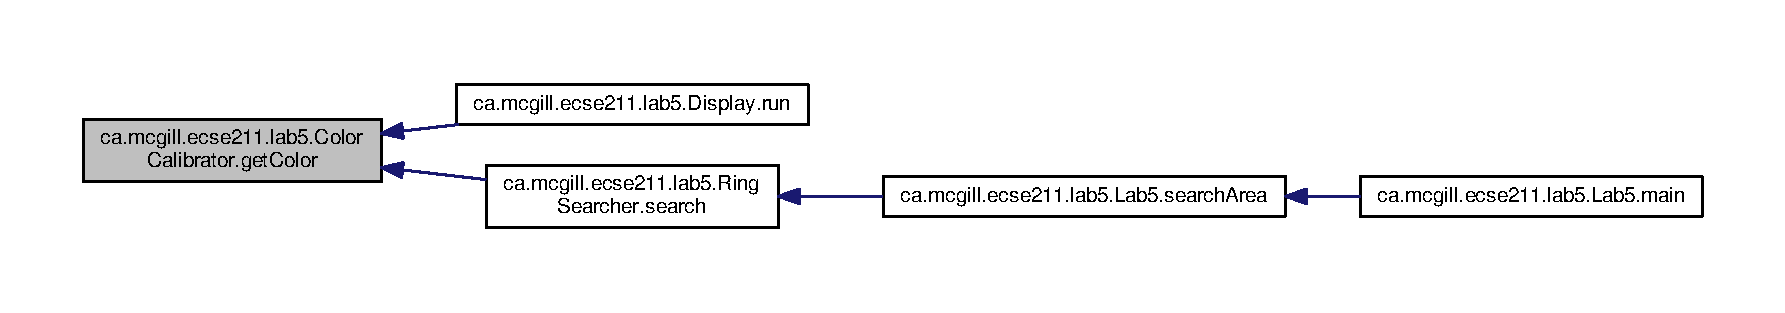
\includegraphics[width=350pt]{classca_1_1mcgill_1_1ecse211_1_1lab5_1_1_color_calibrator_a115188f4d3b465e09db3482f8a6f25d2_icgraph}
\end{center}
\end{figure}
\mbox{\Hypertarget{classca_1_1mcgill_1_1ecse211_1_1lab5_1_1_color_calibrator_ac6a2e41db5bd91b1356f53106178862e}\label{classca_1_1mcgill_1_1ecse211_1_1lab5_1_1_color_calibrator_ac6a2e41db5bd91b1356f53106178862e}} 
\index{ca\+::mcgill\+::ecse211\+::lab5\+::\+Color\+Calibrator@{ca\+::mcgill\+::ecse211\+::lab5\+::\+Color\+Calibrator}!get\+Color@{get\+Color}}
\index{get\+Color@{get\+Color}!ca\+::mcgill\+::ecse211\+::lab5\+::\+Color\+Calibrator@{ca\+::mcgill\+::ecse211\+::lab5\+::\+Color\+Calibrator}}
\subsubsection{\texorpdfstring{get\+Color()}{getColor()}\hspace{0.1cm}{\footnotesize\ttfamily [2/2]}}
{\footnotesize\ttfamily static Color ca.\+mcgill.\+ecse211.\+lab5.\+Color\+Calibrator.\+get\+Color (\begin{DoxyParamCaption}{ }\end{DoxyParamCaption})\hspace{0.3cm}{\ttfamily [static]}}

This method gets the last color of the ring under the light sensor

\begin{DoxyReturn}{Returns}
A Color enumeration value 
\end{DoxyReturn}


Definition at line 66 of file Color\+Calibrator.\+java.



The documentation for this class was generated from the following file\+:\begin{DoxyCompactItemize}
\item 
/home/ccc/\+Eclipse-\/\+Workspace-\/\+Oxygen/\+Lab5-\/\+Search\+And\+Localize/src/ca/mcgill/ecse211/lab5/Color\+Calibrator.\+java\end{DoxyCompactItemize}

\hypertarget{classca_1_1mcgill_1_1ecse211_1_1lab5_1_1_display}{}\section{ca.\+mcgill.\+ecse211.\+lab5.\+Display Class Reference}
\label{classca_1_1mcgill_1_1ecse211_1_1lab5_1_1_display}\index{ca.\+mcgill.\+ecse211.\+lab5.\+Display@{ca.\+mcgill.\+ecse211.\+lab5.\+Display}}


Inheritance diagram for ca.\+mcgill.\+ecse211.\+lab5.\+Display\+:\nopagebreak
\begin{figure}[H]
\begin{center}
\leavevmode
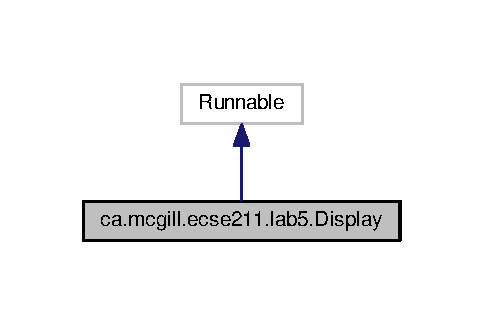
\includegraphics[width=232pt]{classca_1_1mcgill_1_1ecse211_1_1lab5_1_1_display__inherit__graph}
\end{center}
\end{figure}


Collaboration diagram for ca.\+mcgill.\+ecse211.\+lab5.\+Display\+:\nopagebreak
\begin{figure}[H]
\begin{center}
\leavevmode
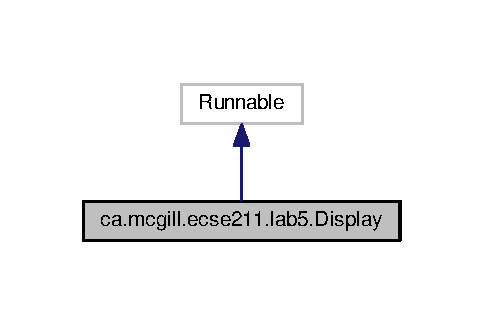
\includegraphics[width=232pt]{classca_1_1mcgill_1_1ecse211_1_1lab5_1_1_display__coll__graph}
\end{center}
\end{figure}
\subsection*{Public Member Functions}
\begin{DoxyCompactItemize}
\item 
\hyperlink{classca_1_1mcgill_1_1ecse211_1_1lab5_1_1_display_aeb15906f02c60c1ca449d4c37922739b}{Display} (Text\+L\+CD lcd)  throws Odometer\+Exceptions 
\item 
\hyperlink{classca_1_1mcgill_1_1ecse211_1_1lab5_1_1_display_abb1c01962b84cfad6ff897ce490b365a}{Display} (Text\+L\+CD lcd, long timeout)  throws Odometer\+Exceptions 
\item 
void \hyperlink{classca_1_1mcgill_1_1ecse211_1_1lab5_1_1_display_a047e885f7170ba80f60fd3b4b2bc79a9}{run} ()
\end{DoxyCompactItemize}


\subsection{Detailed Description}
This class is used to display the content of the odometer variables (x, y, Theta)

\begin{DoxyAuthor}{Author}
Caspar Cedro 

Percy Chen 

Patrick Erath 

Anssam Ghezala 

Susan Matuszewski 

Kamy Moussavi Kafi 
\end{DoxyAuthor}


Definition at line 19 of file Display.\+java.



\subsection{Constructor \& Destructor Documentation}
\mbox{\Hypertarget{classca_1_1mcgill_1_1ecse211_1_1lab5_1_1_display_aeb15906f02c60c1ca449d4c37922739b}\label{classca_1_1mcgill_1_1ecse211_1_1lab5_1_1_display_aeb15906f02c60c1ca449d4c37922739b}} 
\index{ca\+::mcgill\+::ecse211\+::lab5\+::\+Display@{ca\+::mcgill\+::ecse211\+::lab5\+::\+Display}!Display@{Display}}
\index{Display@{Display}!ca\+::mcgill\+::ecse211\+::lab5\+::\+Display@{ca\+::mcgill\+::ecse211\+::lab5\+::\+Display}}
\subsubsection{\texorpdfstring{Display()}{Display()}\hspace{0.1cm}{\footnotesize\ttfamily [1/2]}}
{\footnotesize\ttfamily ca.\+mcgill.\+ecse211.\+lab5.\+Display.\+Display (\begin{DoxyParamCaption}\item[{Text\+L\+CD}]{lcd }\end{DoxyParamCaption}) throws \hyperlink{classca_1_1mcgill_1_1ecse211_1_1odometer_1_1_odometer_exceptions}{Odometer\+Exceptions}}

This is the class constructor for a display object that controls an E\+V3 brick display


\begin{DoxyParams}{Parameters}
{\em lcd} & A Text\+L\+CD object instance to control \\
\hline
\end{DoxyParams}

\begin{DoxyExceptions}{Exceptions}
{\em Odometer\+Exceptions} & \\
\hline
\end{DoxyExceptions}


Definition at line 35 of file Display.\+java.

Here is the call graph for this function\+:\nopagebreak
\begin{figure}[H]
\begin{center}
\leavevmode
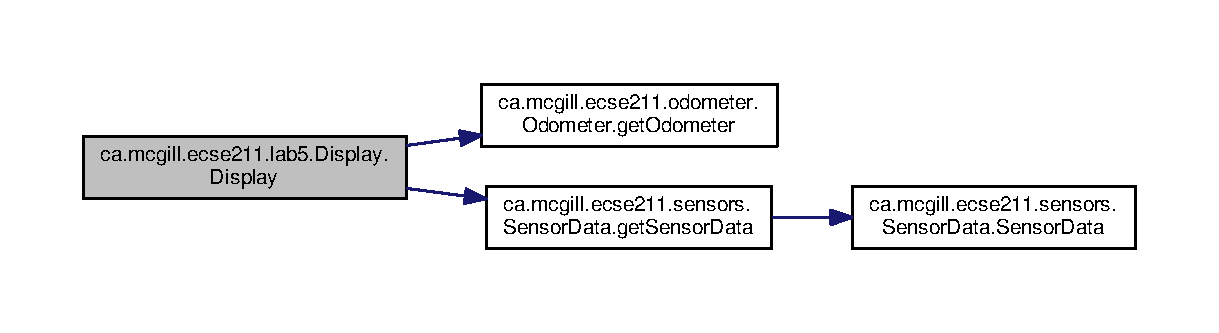
\includegraphics[width=350pt]{classca_1_1mcgill_1_1ecse211_1_1lab5_1_1_display_aeb15906f02c60c1ca449d4c37922739b_cgraph}
\end{center}
\end{figure}
\mbox{\Hypertarget{classca_1_1mcgill_1_1ecse211_1_1lab5_1_1_display_abb1c01962b84cfad6ff897ce490b365a}\label{classca_1_1mcgill_1_1ecse211_1_1lab5_1_1_display_abb1c01962b84cfad6ff897ce490b365a}} 
\index{ca\+::mcgill\+::ecse211\+::lab5\+::\+Display@{ca\+::mcgill\+::ecse211\+::lab5\+::\+Display}!Display@{Display}}
\index{Display@{Display}!ca\+::mcgill\+::ecse211\+::lab5\+::\+Display@{ca\+::mcgill\+::ecse211\+::lab5\+::\+Display}}
\subsubsection{\texorpdfstring{Display()}{Display()}\hspace{0.1cm}{\footnotesize\ttfamily [2/2]}}
{\footnotesize\ttfamily ca.\+mcgill.\+ecse211.\+lab5.\+Display.\+Display (\begin{DoxyParamCaption}\item[{Text\+L\+CD}]{lcd,  }\item[{long}]{timeout }\end{DoxyParamCaption}) throws \hyperlink{classca_1_1mcgill_1_1ecse211_1_1odometer_1_1_odometer_exceptions}{Odometer\+Exceptions}}

This is the overloaded class constructor for a display object


\begin{DoxyParams}{Parameters}
{\em lcd} & A Text\+L\+CD object instance to control \\
\hline
{\em timeout} & A duration of time to update the display for \\
\hline
\end{DoxyParams}

\begin{DoxyExceptions}{Exceptions}
{\em Odometer\+Exceptions} & \\
\hline
\end{DoxyExceptions}


Definition at line 48 of file Display.\+java.

Here is the call graph for this function\+:\nopagebreak
\begin{figure}[H]
\begin{center}
\leavevmode
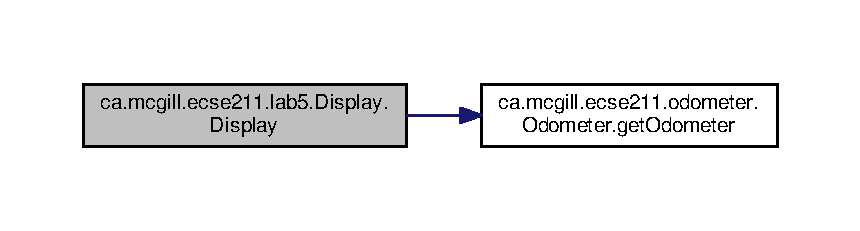
\includegraphics[width=350pt]{classca_1_1mcgill_1_1ecse211_1_1lab5_1_1_display_abb1c01962b84cfad6ff897ce490b365a_cgraph}
\end{center}
\end{figure}


\subsection{Member Function Documentation}
\mbox{\Hypertarget{classca_1_1mcgill_1_1ecse211_1_1lab5_1_1_display_a047e885f7170ba80f60fd3b4b2bc79a9}\label{classca_1_1mcgill_1_1ecse211_1_1lab5_1_1_display_a047e885f7170ba80f60fd3b4b2bc79a9}} 
\index{ca\+::mcgill\+::ecse211\+::lab5\+::\+Display@{ca\+::mcgill\+::ecse211\+::lab5\+::\+Display}!run@{run}}
\index{run@{run}!ca\+::mcgill\+::ecse211\+::lab5\+::\+Display@{ca\+::mcgill\+::ecse211\+::lab5\+::\+Display}}
\subsubsection{\texorpdfstring{run()}{run()}}
{\footnotesize\ttfamily void ca.\+mcgill.\+ecse211.\+lab5.\+Display.\+run (\begin{DoxyParamCaption}{ }\end{DoxyParamCaption})}

This method is called when the \hyperlink{classca_1_1mcgill_1_1ecse211_1_1lab5_1_1_display}{Display} thread is started. 

Definition at line 57 of file Display.\+java.

Here is the call graph for this function\+:
\nopagebreak
\begin{figure}[H]
\begin{center}
\leavevmode
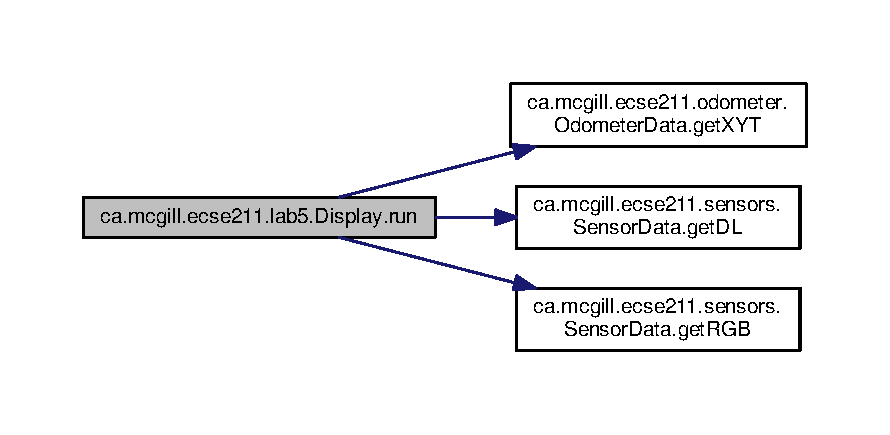
\includegraphics[width=350pt]{classca_1_1mcgill_1_1ecse211_1_1lab5_1_1_display_a047e885f7170ba80f60fd3b4b2bc79a9_cgraph}
\end{center}
\end{figure}


The documentation for this class was generated from the following file\+:\begin{DoxyCompactItemize}
\item 
/home/ccc/\+Eclipse-\/\+Workspace-\/\+Oxygen/\+Lab5-\/\+Search\+And\+Localize/src/ca/mcgill/ecse211/lab5/Display.\+java\end{DoxyCompactItemize}

\hypertarget{classca_1_1mcgill_1_1ecse211_1_1sensors_1_1_gyro_poller}{}\section{ca.\+mcgill.\+ecse211.\+sensors.\+Gyro\+Poller Class Reference}
\label{classca_1_1mcgill_1_1ecse211_1_1sensors_1_1_gyro_poller}\index{ca.\+mcgill.\+ecse211.\+sensors.\+Gyro\+Poller@{ca.\+mcgill.\+ecse211.\+sensors.\+Gyro\+Poller}}


Inheritance diagram for ca.\+mcgill.\+ecse211.\+sensors.\+Gyro\+Poller\+:\nopagebreak
\begin{figure}[H]
\begin{center}
\leavevmode
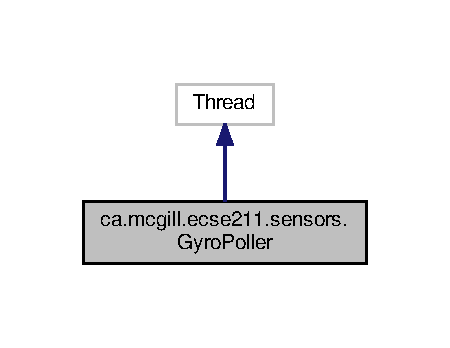
\includegraphics[width=216pt]{classca_1_1mcgill_1_1ecse211_1_1sensors_1_1_gyro_poller__inherit__graph}
\end{center}
\end{figure}


Collaboration diagram for ca.\+mcgill.\+ecse211.\+sensors.\+Gyro\+Poller\+:\nopagebreak
\begin{figure}[H]
\begin{center}
\leavevmode
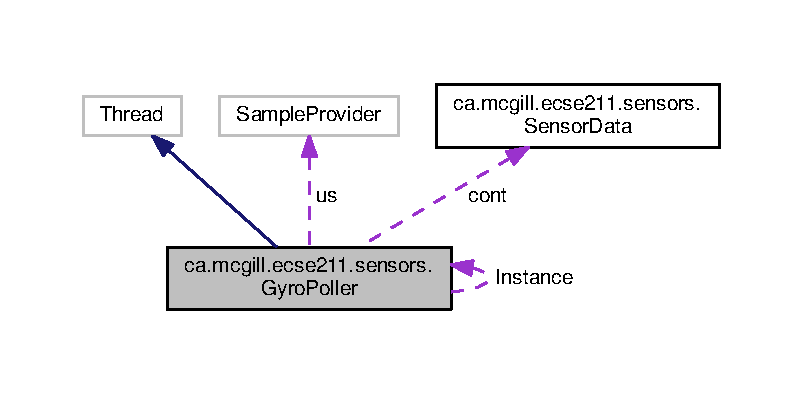
\includegraphics[width=350pt]{classca_1_1mcgill_1_1ecse211_1_1sensors_1_1_gyro_poller__coll__graph}
\end{center}
\end{figure}
\subsection*{Public Member Functions}
\begin{DoxyCompactItemize}
\item 
\hyperlink{classca_1_1mcgill_1_1ecse211_1_1sensors_1_1_gyro_poller_a284eec4434708068ce9cb8a9635f7830}{Gyro\+Poller} (Sample\+Provider us, float\mbox{[}$\,$\mbox{]} lg\+Data, \hyperlink{classca_1_1mcgill_1_1ecse211_1_1sensors_1_1_sensor_data}{Sensor\+Data} cont)  throws Odometer\+Exceptions 
\item 
void \hyperlink{classca_1_1mcgill_1_1ecse211_1_1sensors_1_1_gyro_poller_a2a52059192555ece72190fa44a761d28}{run} ()
\end{DoxyCompactItemize}
\subsection*{Public Attributes}
\begin{DoxyCompactItemize}
\item 
\mbox{\Hypertarget{classca_1_1mcgill_1_1ecse211_1_1sensors_1_1_gyro_poller_a2df6c86572aff4ee54e4b7cfcac1f71b}\label{classca_1_1mcgill_1_1ecse211_1_1sensors_1_1_gyro_poller_a2df6c86572aff4ee54e4b7cfcac1f71b}} 
\hyperlink{classca_1_1mcgill_1_1ecse211_1_1sensors_1_1_gyro_poller}{Gyro\+Poller} {\bfseries Instance}
\end{DoxyCompactItemize}
\subsection*{Protected Member Functions}
\begin{DoxyCompactItemize}
\item 
\mbox{\Hypertarget{classca_1_1mcgill_1_1ecse211_1_1sensors_1_1_gyro_poller_affd8cf8f49c8619b9617445e54e574f6}\label{classca_1_1mcgill_1_1ecse211_1_1sensors_1_1_gyro_poller_affd8cf8f49c8619b9617445e54e574f6}} 
void {\bfseries process\+Data} ()
\end{DoxyCompactItemize}
\subsection*{Protected Attributes}
\begin{DoxyCompactItemize}
\item 
\mbox{\Hypertarget{classca_1_1mcgill_1_1ecse211_1_1sensors_1_1_gyro_poller_a98fc98dff0acec54cec2d14284bd686a}\label{classca_1_1mcgill_1_1ecse211_1_1sensors_1_1_gyro_poller_a98fc98dff0acec54cec2d14284bd686a}} 
Sample\+Provider {\bfseries us}
\item 
\mbox{\Hypertarget{classca_1_1mcgill_1_1ecse211_1_1sensors_1_1_gyro_poller_af938c0d98e85a2b52a892b3060a16e55}\label{classca_1_1mcgill_1_1ecse211_1_1sensors_1_1_gyro_poller_af938c0d98e85a2b52a892b3060a16e55}} 
\hyperlink{classca_1_1mcgill_1_1ecse211_1_1sensors_1_1_sensor_data}{Sensor\+Data} {\bfseries cont}
\item 
\mbox{\Hypertarget{classca_1_1mcgill_1_1ecse211_1_1sensors_1_1_gyro_poller_a6e6759875b42b8ac6947aac140e74fce}\label{classca_1_1mcgill_1_1ecse211_1_1sensors_1_1_gyro_poller_a6e6759875b42b8ac6947aac140e74fce}} 
float \mbox{[}$\,$\mbox{]} {\bfseries lg\+Data}
\end{DoxyCompactItemize}


\subsection{Detailed Description}
This class helps our robot to navigate using a gyroscope

\begin{DoxyAuthor}{Author}
Caspar Cedro 

Percy Chen 

Patrick Erath 

Anssam Ghezala 

Susan Matuszewski 

Kamy Moussavi Kafi 
\end{DoxyAuthor}


Definition at line 16 of file Gyro\+Poller.\+java.



\subsection{Constructor \& Destructor Documentation}
\mbox{\Hypertarget{classca_1_1mcgill_1_1ecse211_1_1sensors_1_1_gyro_poller_a284eec4434708068ce9cb8a9635f7830}\label{classca_1_1mcgill_1_1ecse211_1_1sensors_1_1_gyro_poller_a284eec4434708068ce9cb8a9635f7830}} 
\index{ca\+::mcgill\+::ecse211\+::sensors\+::\+Gyro\+Poller@{ca\+::mcgill\+::ecse211\+::sensors\+::\+Gyro\+Poller}!Gyro\+Poller@{Gyro\+Poller}}
\index{Gyro\+Poller@{Gyro\+Poller}!ca\+::mcgill\+::ecse211\+::sensors\+::\+Gyro\+Poller@{ca\+::mcgill\+::ecse211\+::sensors\+::\+Gyro\+Poller}}
\subsubsection{\texorpdfstring{Gyro\+Poller()}{GyroPoller()}}
{\footnotesize\ttfamily ca.\+mcgill.\+ecse211.\+sensors.\+Gyro\+Poller.\+Gyro\+Poller (\begin{DoxyParamCaption}\item[{Sample\+Provider}]{us,  }\item[{float \mbox{[}$\,$\mbox{]}}]{lg\+Data,  }\item[{\hyperlink{classca_1_1mcgill_1_1ecse211_1_1sensors_1_1_sensor_data}{Sensor\+Data}}]{cont }\end{DoxyParamCaption}) throws \hyperlink{classca_1_1mcgill_1_1ecse211_1_1odometer_1_1_odometer_exceptions}{Odometer\+Exceptions}}

This constructor creates an instance of the \hyperlink{classca_1_1mcgill_1_1ecse211_1_1sensors_1_1_gyro_poller}{Gyro\+Poller} class to aid navigation


\begin{DoxyParams}{Parameters}
{\em us} & A Sample\+Provider class instance that helps us to store an array of ultrasonic sensor data. \\
\hline
{\em lg\+Data} & An array used to store data. \\
\hline
{\em cont} & A \hyperlink{classca_1_1mcgill_1_1ecse211_1_1sensors_1_1_sensor_data}{Sensor\+Data} object instance used to manage sensor data. \\
\hline
\end{DoxyParams}

\begin{DoxyExceptions}{Exceptions}
{\em Odometer\+Exceptions} & \\
\hline
\end{DoxyExceptions}


Definition at line 31 of file Gyro\+Poller.\+java.



\subsection{Member Function Documentation}
\mbox{\Hypertarget{classca_1_1mcgill_1_1ecse211_1_1sensors_1_1_gyro_poller_a2a52059192555ece72190fa44a761d28}\label{classca_1_1mcgill_1_1ecse211_1_1sensors_1_1_gyro_poller_a2a52059192555ece72190fa44a761d28}} 
\index{ca\+::mcgill\+::ecse211\+::sensors\+::\+Gyro\+Poller@{ca\+::mcgill\+::ecse211\+::sensors\+::\+Gyro\+Poller}!run@{run}}
\index{run@{run}!ca\+::mcgill\+::ecse211\+::sensors\+::\+Gyro\+Poller@{ca\+::mcgill\+::ecse211\+::sensors\+::\+Gyro\+Poller}}
\subsubsection{\texorpdfstring{run()}{run()}}
{\footnotesize\ttfamily void ca.\+mcgill.\+ecse211.\+sensors.\+Gyro\+Poller.\+run (\begin{DoxyParamCaption}{ }\end{DoxyParamCaption})}

This method is called by a \hyperlink{classca_1_1mcgill_1_1ecse211_1_1sensors_1_1_ultrasonic_poller}{Ultrasonic\+Poller} (Thread) instance when it is asked to start executing

Sensors now return floats using a uniform protocol. Need to convert US result to an integer \mbox{[}0,255\mbox{]} (non-\/\+Javadoc)

\begin{DoxySeeAlso}{See also}
java.\+lang.\+Thread\+::run() 
\end{DoxySeeAlso}


Definition at line 46 of file Gyro\+Poller.\+java.

Here is the call graph for this function\+:\nopagebreak
\begin{figure}[H]
\begin{center}
\leavevmode
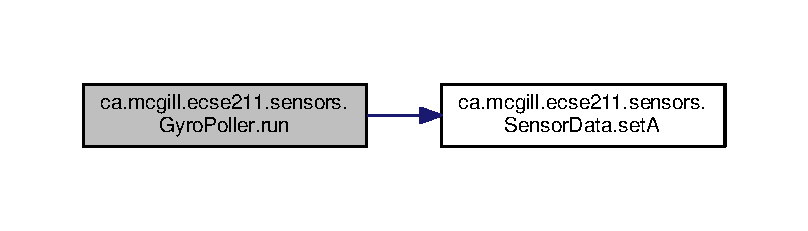
\includegraphics[width=350pt]{classca_1_1mcgill_1_1ecse211_1_1sensors_1_1_gyro_poller_a2a52059192555ece72190fa44a761d28_cgraph}
\end{center}
\end{figure}


The documentation for this class was generated from the following file\+:\begin{DoxyCompactItemize}
\item 
/home/ccc/\+Eclipse-\/\+Workspace-\/\+Oxygen/\+Lab5-\/\+Search\+And\+Localize/src/ca/mcgill/ecse211/sensors/Gyro\+Poller.\+java\end{DoxyCompactItemize}

\hypertarget{classca_1_1mcgill_1_1ecse211_1_1lab5_1_1_lab5}{}\section{ca.\+mcgill.\+ecse211.\+lab5.\+Lab5 Class Reference}
\label{classca_1_1mcgill_1_1ecse211_1_1lab5_1_1_lab5}\index{ca.\+mcgill.\+ecse211.\+lab5.\+Lab5@{ca.\+mcgill.\+ecse211.\+lab5.\+Lab5}}


Collaboration diagram for ca.\+mcgill.\+ecse211.\+lab5.\+Lab5\+:
\nopagebreak
\begin{figure}[H]
\begin{center}
\leavevmode
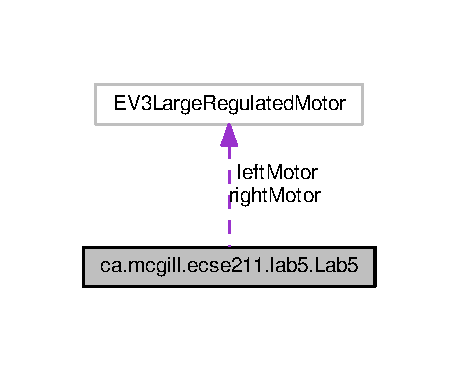
\includegraphics[width=350pt]{classca_1_1mcgill_1_1ecse211_1_1lab5_1_1_lab5__coll__graph}
\end{center}
\end{figure}
\subsection*{Static Public Member Functions}
\begin{DoxyCompactItemize}
\item 
static void \hyperlink{classca_1_1mcgill_1_1ecse211_1_1lab5_1_1_lab5_a82cca51f550ed0eb016bb2082d3fe755}{main} (String\mbox{[}$\,$\mbox{]} args)  throws Odometer\+Exceptions 
\item 
static void \hyperlink{classca_1_1mcgill_1_1ecse211_1_1lab5_1_1_lab5_a0e80ac0068ef1ab41cfb571b8c65845c}{search\+Area} (\hyperlink{classca_1_1mcgill_1_1ecse211_1_1lab5_1_1_navigation}{Navigation} navigation, \hyperlink{classca_1_1mcgill_1_1ecse211_1_1lab5_1_1_ring_searcher}{Ring\+Searcher} searcher, Color\+Calibrator.\+Color target\+Color)
\end{DoxyCompactItemize}
\subsection*{Static Public Attributes}
\begin{DoxyCompactItemize}
\item 
static Port \hyperlink{classca_1_1mcgill_1_1ecse211_1_1lab5_1_1_lab5_a2415c0078b42b8813c3cc9304d6335ce}{g\+Port} = Local\+E\+V3.\+get().get\+Port(\char`\"{}S4\char`\"{})
\item 
static E\+V3\+Gyro\+Sensor \hyperlink{classca_1_1mcgill_1_1ecse211_1_1lab5_1_1_lab5_a0e63e3a6920344136ebfa14780670ee3}{g\+Sensor}
\item 
static final E\+V3\+Large\+Regulated\+Motor \hyperlink{classca_1_1mcgill_1_1ecse211_1_1lab5_1_1_lab5_a613e69d8f1e90a1161b78020571110fc}{left\+Motor}
\item 
static final E\+V3\+Large\+Regulated\+Motor \hyperlink{classca_1_1mcgill_1_1ecse211_1_1lab5_1_1_lab5_a70575e1c6e84cd9d22cadd141ad6ceae}{right\+Motor}
\item 
static final double \hyperlink{classca_1_1mcgill_1_1ecse211_1_1lab5_1_1_lab5_a099ba21be1cd8d54a57c40cd0d35701d}{T\+I\+LE} = 30.\+48
\item 
static final double \hyperlink{classca_1_1mcgill_1_1ecse211_1_1lab5_1_1_lab5_ab9b6fc96d3fb1ac6c7d69d1727b3bbdd}{W\+H\+E\+E\+L\+\_\+\+R\+AD} = 2.\+2
\item 
static final double \hyperlink{classca_1_1mcgill_1_1ecse211_1_1lab5_1_1_lab5_a3d2e7eb578ce6ef7f7453feed3835e1d}{T\+R\+A\+CK} = 10.\+8
\item 
static final int \mbox{[}$\,$\mbox{]} \hyperlink{classca_1_1mcgill_1_1ecse211_1_1lab5_1_1_lab5_a39cbd32759fdb575b92b694f2713085d}{SC} = \{1, 1\}
\item 
static final int \hyperlink{classca_1_1mcgill_1_1ecse211_1_1lab5_1_1_lab5_a0dd5ea6f697d2221ed8c8bb4df1cac7f}{TR} = 1
\item 
static final int \hyperlink{classca_1_1mcgill_1_1ecse211_1_1lab5_1_1_lab5_a957a526ed669e9d8b7fc485e21385ee9}{L\+Lx} = 3
\item 
static boolean \mbox{[}$\,$\mbox{]}\mbox{[}$\,$\mbox{]} \hyperlink{classca_1_1mcgill_1_1ecse211_1_1lab5_1_1_lab5_a27ae00bb6fbeed54573af9cc5c3dc32e}{visited\+Search\+Area\+Coordinates}
\end{DoxyCompactItemize}


\subsection{Detailed Description}
This class implements the main starting point for the Search and Localize lab

\begin{DoxyAuthor}{Author}
Caspar Cedro \& Percy Chen \& Patrick Erath \& Anssam Ghezala \& Susan Matuszewski \& Kamy Moussavi Kafi 
\end{DoxyAuthor}


Definition at line 28 of file Lab5.\+java.



\subsection{Member Function Documentation}
\mbox{\Hypertarget{classca_1_1mcgill_1_1ecse211_1_1lab5_1_1_lab5_a82cca51f550ed0eb016bb2082d3fe755}\label{classca_1_1mcgill_1_1ecse211_1_1lab5_1_1_lab5_a82cca51f550ed0eb016bb2082d3fe755}} 
\index{ca\+::mcgill\+::ecse211\+::lab5\+::\+Lab5@{ca\+::mcgill\+::ecse211\+::lab5\+::\+Lab5}!main@{main}}
\index{main@{main}!ca\+::mcgill\+::ecse211\+::lab5\+::\+Lab5@{ca\+::mcgill\+::ecse211\+::lab5\+::\+Lab5}}
\subsubsection{\texorpdfstring{main()}{main()}}
{\footnotesize\ttfamily static void ca.\+mcgill.\+ecse211.\+lab5.\+Lab5.\+main (\begin{DoxyParamCaption}\item[{String \mbox{[}$\,$\mbox{]}}]{args }\end{DoxyParamCaption}) throws \hyperlink{classca_1_1mcgill_1_1ecse211_1_1odometer_1_1_odometer_exceptions}{Odometer\+Exceptions}\hspace{0.3cm}{\ttfamily [static]}}

This method is our main entry point -\/ instantiate objects used and set up sensor.


\begin{DoxyParams}{Parameters}
{\em args} & an array of arguments that can be passed in via commandline or otherwise. \\
\hline
\end{DoxyParams}


Definition at line 102 of file Lab5.\+java.

Here is the call graph for this function\+:
\nopagebreak
\begin{figure}[H]
\begin{center}
\leavevmode
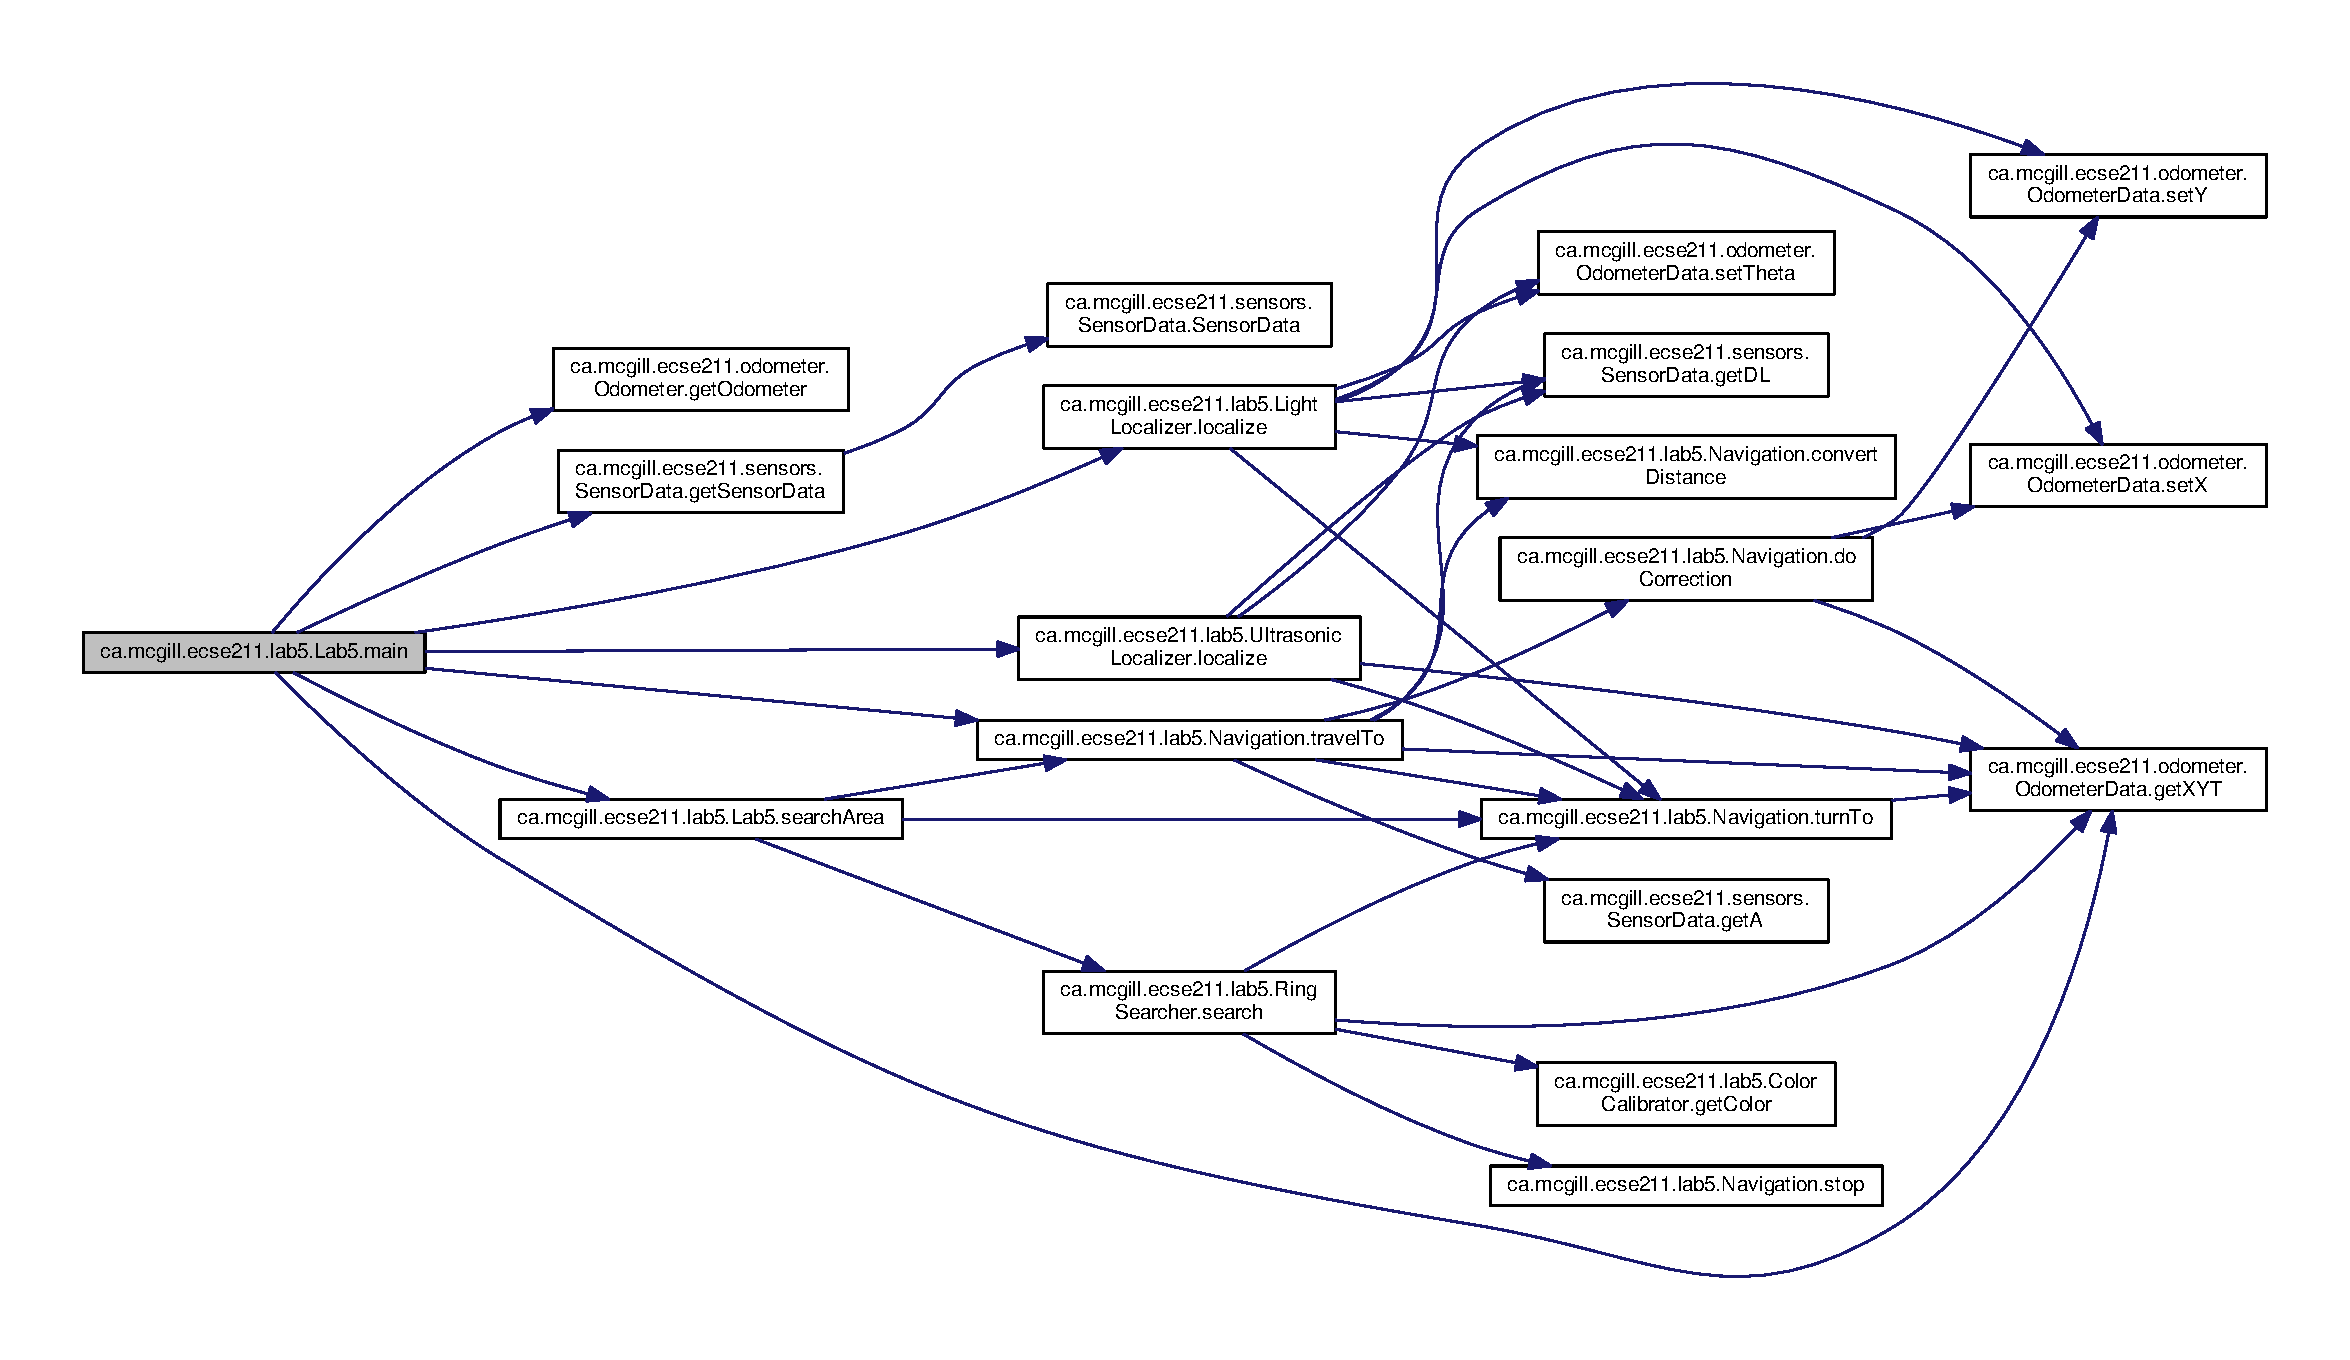
\includegraphics[width=350pt]{classca_1_1mcgill_1_1ecse211_1_1lab5_1_1_lab5_a82cca51f550ed0eb016bb2082d3fe755_cgraph}
\end{center}
\end{figure}
\mbox{\Hypertarget{classca_1_1mcgill_1_1ecse211_1_1lab5_1_1_lab5_a0e80ac0068ef1ab41cfb571b8c65845c}\label{classca_1_1mcgill_1_1ecse211_1_1lab5_1_1_lab5_a0e80ac0068ef1ab41cfb571b8c65845c}} 
\index{ca\+::mcgill\+::ecse211\+::lab5\+::\+Lab5@{ca\+::mcgill\+::ecse211\+::lab5\+::\+Lab5}!search\+Area@{search\+Area}}
\index{search\+Area@{search\+Area}!ca\+::mcgill\+::ecse211\+::lab5\+::\+Lab5@{ca\+::mcgill\+::ecse211\+::lab5\+::\+Lab5}}
\subsubsection{\texorpdfstring{search\+Area()}{searchArea()}}
{\footnotesize\ttfamily static void ca.\+mcgill.\+ecse211.\+lab5.\+Lab5.\+search\+Area (\begin{DoxyParamCaption}\item[{\hyperlink{classca_1_1mcgill_1_1ecse211_1_1lab5_1_1_navigation}{Navigation}}]{navigation,  }\item[{\hyperlink{classca_1_1mcgill_1_1ecse211_1_1lab5_1_1_ring_searcher}{Ring\+Searcher}}]{searcher,  }\item[{Color\+Calibrator.\+Color}]{target\+Color }\end{DoxyParamCaption})\hspace{0.3cm}{\ttfamily [static]}}

This method finished the search process, it returns when it find the targeted run


\begin{DoxyParams}{Parameters}
{\em navigation} & A \hyperlink{classca_1_1mcgill_1_1ecse211_1_1lab5_1_1_navigation}{Navigation} class object instance to aid the robot navigate the grid \\
\hline
{\em searcher} & A \hyperlink{classca_1_1mcgill_1_1ecse211_1_1lab5_1_1_ring_searcher}{Ring\+Searcher} class object instance with methods that search for a ring \\
\hline
{\em target\+Color} & The color of the ring that the robot should search for \\
\hline
\end{DoxyParams}


Definition at line 214 of file Lab5.\+java.

Here is the call graph for this function\+:
\nopagebreak
\begin{figure}[H]
\begin{center}
\leavevmode
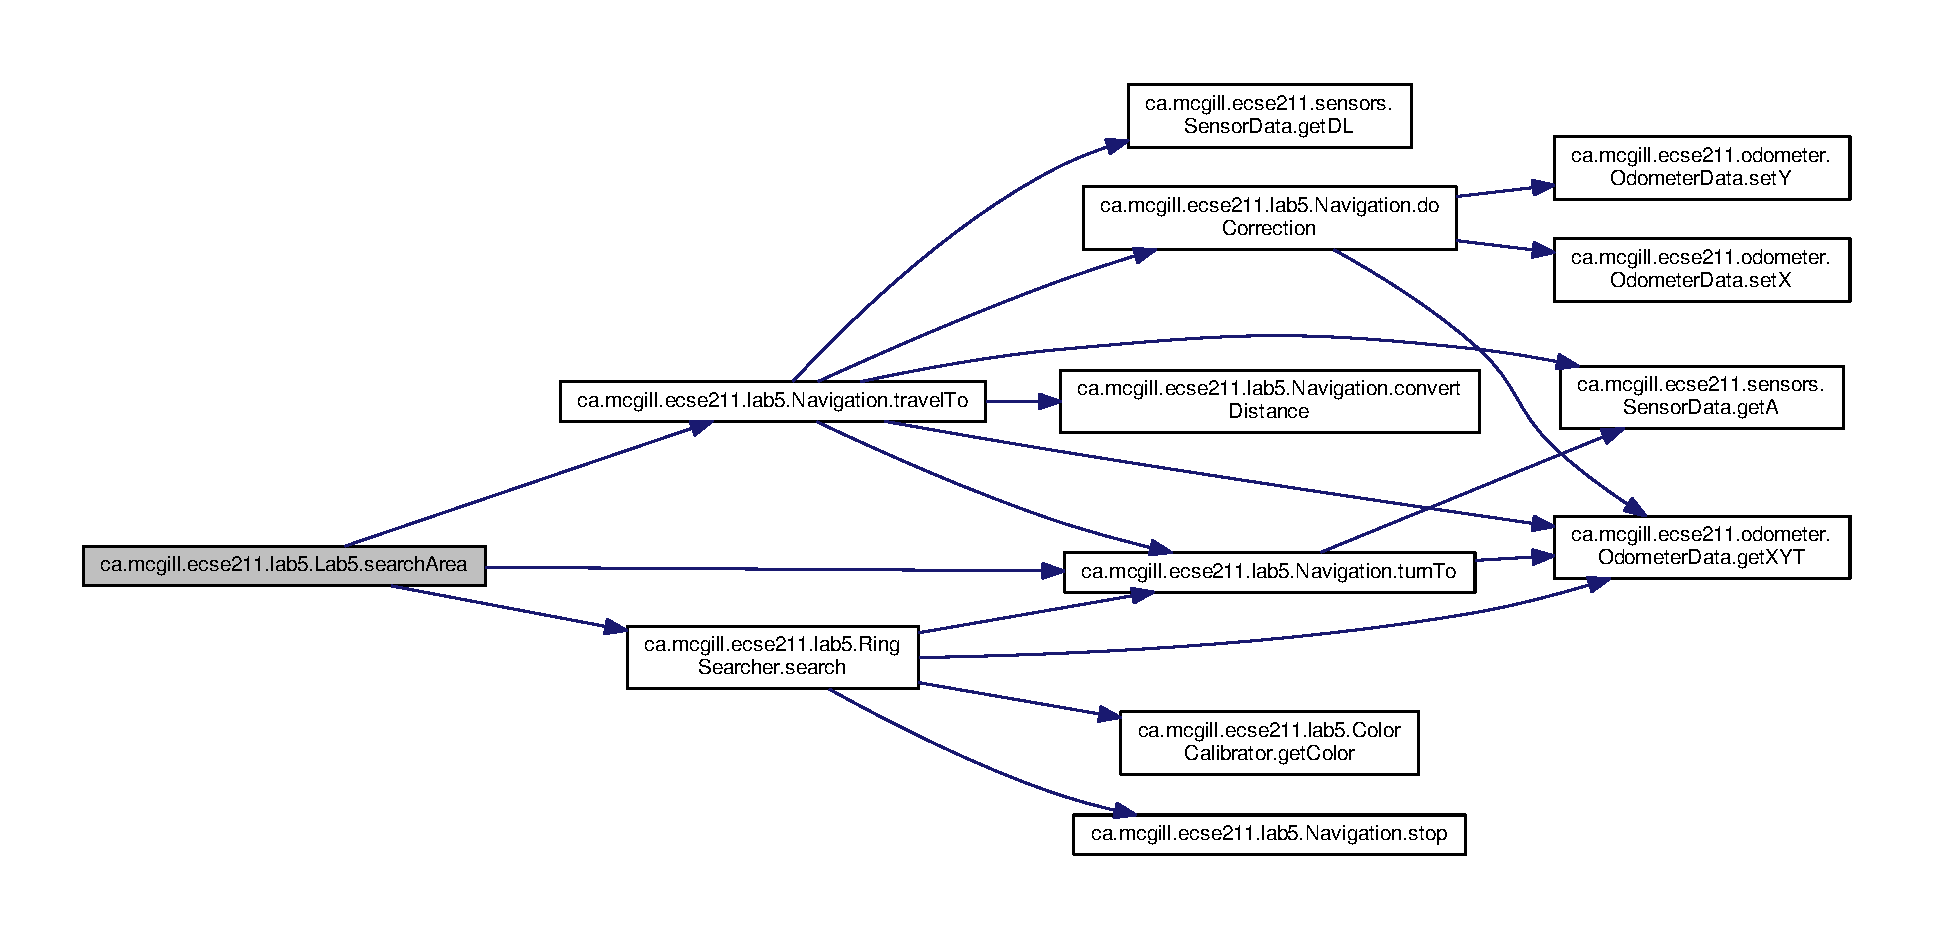
\includegraphics[width=350pt]{classca_1_1mcgill_1_1ecse211_1_1lab5_1_1_lab5_a0e80ac0068ef1ab41cfb571b8c65845c_cgraph}
\end{center}
\end{figure}
Here is the caller graph for this function\+:
\nopagebreak
\begin{figure}[H]
\begin{center}
\leavevmode
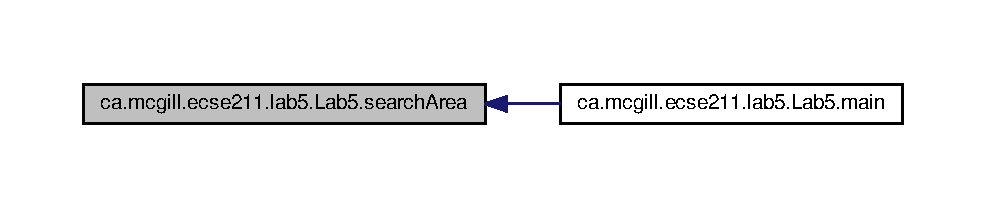
\includegraphics[width=350pt]{classca_1_1mcgill_1_1ecse211_1_1lab5_1_1_lab5_a0e80ac0068ef1ab41cfb571b8c65845c_icgraph}
\end{center}
\end{figure}


\subsection{Member Data Documentation}
\mbox{\Hypertarget{classca_1_1mcgill_1_1ecse211_1_1lab5_1_1_lab5_a2415c0078b42b8813c3cc9304d6335ce}\label{classca_1_1mcgill_1_1ecse211_1_1lab5_1_1_lab5_a2415c0078b42b8813c3cc9304d6335ce}} 
\index{ca\+::mcgill\+::ecse211\+::lab5\+::\+Lab5@{ca\+::mcgill\+::ecse211\+::lab5\+::\+Lab5}!g\+Port@{g\+Port}}
\index{g\+Port@{g\+Port}!ca\+::mcgill\+::ecse211\+::lab5\+::\+Lab5@{ca\+::mcgill\+::ecse211\+::lab5\+::\+Lab5}}
\subsubsection{\texorpdfstring{g\+Port}{gPort}}
{\footnotesize\ttfamily Port ca.\+mcgill.\+ecse211.\+lab5.\+Lab5.\+g\+Port = Local\+E\+V3.\+get().get\+Port(\char`\"{}S4\char`\"{})\hspace{0.3cm}{\ttfamily [static]}}

Port object instance for our gyroscope sensor 

Definition at line 39 of file Lab5.\+java.

\mbox{\Hypertarget{classca_1_1mcgill_1_1ecse211_1_1lab5_1_1_lab5_a0e63e3a6920344136ebfa14780670ee3}\label{classca_1_1mcgill_1_1ecse211_1_1lab5_1_1_lab5_a0e63e3a6920344136ebfa14780670ee3}} 
\index{ca\+::mcgill\+::ecse211\+::lab5\+::\+Lab5@{ca\+::mcgill\+::ecse211\+::lab5\+::\+Lab5}!g\+Sensor@{g\+Sensor}}
\index{g\+Sensor@{g\+Sensor}!ca\+::mcgill\+::ecse211\+::lab5\+::\+Lab5@{ca\+::mcgill\+::ecse211\+::lab5\+::\+Lab5}}
\subsubsection{\texorpdfstring{g\+Sensor}{gSensor}}
{\footnotesize\ttfamily E\+V3\+Gyro\+Sensor ca.\+mcgill.\+ecse211.\+lab5.\+Lab5.\+g\+Sensor\hspace{0.3cm}{\ttfamily [static]}}

E\+V3\+Gyro\+Sensor object instance for our gyroscope sensor 

Definition at line 44 of file Lab5.\+java.

\mbox{\Hypertarget{classca_1_1mcgill_1_1ecse211_1_1lab5_1_1_lab5_a613e69d8f1e90a1161b78020571110fc}\label{classca_1_1mcgill_1_1ecse211_1_1lab5_1_1_lab5_a613e69d8f1e90a1161b78020571110fc}} 
\index{ca\+::mcgill\+::ecse211\+::lab5\+::\+Lab5@{ca\+::mcgill\+::ecse211\+::lab5\+::\+Lab5}!left\+Motor@{left\+Motor}}
\index{left\+Motor@{left\+Motor}!ca\+::mcgill\+::ecse211\+::lab5\+::\+Lab5@{ca\+::mcgill\+::ecse211\+::lab5\+::\+Lab5}}
\subsubsection{\texorpdfstring{left\+Motor}{leftMotor}}
{\footnotesize\ttfamily final E\+V3\+Large\+Regulated\+Motor ca.\+mcgill.\+ecse211.\+lab5.\+Lab5.\+left\+Motor\hspace{0.3cm}{\ttfamily [static]}}

{\bfseries Initial value\+:}
\begin{DoxyCode}
=
      \textcolor{keyword}{new} EV3LargeRegulatedMotor(LocalEV3.get().getPort(\textcolor{stringliteral}{"A"}))
\end{DoxyCode}
Motor object instance that allows control of the left motor connected to port B 

Definition at line 49 of file Lab5.\+java.

\mbox{\Hypertarget{classca_1_1mcgill_1_1ecse211_1_1lab5_1_1_lab5_a957a526ed669e9d8b7fc485e21385ee9}\label{classca_1_1mcgill_1_1ecse211_1_1lab5_1_1_lab5_a957a526ed669e9d8b7fc485e21385ee9}} 
\index{ca\+::mcgill\+::ecse211\+::lab5\+::\+Lab5@{ca\+::mcgill\+::ecse211\+::lab5\+::\+Lab5}!L\+Lx@{L\+Lx}}
\index{L\+Lx@{L\+Lx}!ca\+::mcgill\+::ecse211\+::lab5\+::\+Lab5@{ca\+::mcgill\+::ecse211\+::lab5\+::\+Lab5}}
\subsubsection{\texorpdfstring{L\+Lx}{LLx}}
{\footnotesize\ttfamily final int ca.\+mcgill.\+ecse211.\+lab5.\+Lab5.\+L\+Lx = 3\hspace{0.3cm}{\ttfamily [static]}}

These are the coordinates for our search area. LL = Lower Left UR = Upper Right 

Definition at line 88 of file Lab5.\+java.

\mbox{\Hypertarget{classca_1_1mcgill_1_1ecse211_1_1lab5_1_1_lab5_a70575e1c6e84cd9d22cadd141ad6ceae}\label{classca_1_1mcgill_1_1ecse211_1_1lab5_1_1_lab5_a70575e1c6e84cd9d22cadd141ad6ceae}} 
\index{ca\+::mcgill\+::ecse211\+::lab5\+::\+Lab5@{ca\+::mcgill\+::ecse211\+::lab5\+::\+Lab5}!right\+Motor@{right\+Motor}}
\index{right\+Motor@{right\+Motor}!ca\+::mcgill\+::ecse211\+::lab5\+::\+Lab5@{ca\+::mcgill\+::ecse211\+::lab5\+::\+Lab5}}
\subsubsection{\texorpdfstring{right\+Motor}{rightMotor}}
{\footnotesize\ttfamily final E\+V3\+Large\+Regulated\+Motor ca.\+mcgill.\+ecse211.\+lab5.\+Lab5.\+right\+Motor\hspace{0.3cm}{\ttfamily [static]}}

{\bfseries Initial value\+:}
\begin{DoxyCode}
=
      \textcolor{keyword}{new} EV3LargeRegulatedMotor(LocalEV3.get().getPort(\textcolor{stringliteral}{"D"}))
\end{DoxyCode}
Motor object instance that allows control of the right motor connected to port A 

Definition at line 55 of file Lab5.\+java.

\mbox{\Hypertarget{classca_1_1mcgill_1_1ecse211_1_1lab5_1_1_lab5_a39cbd32759fdb575b92b694f2713085d}\label{classca_1_1mcgill_1_1ecse211_1_1lab5_1_1_lab5_a39cbd32759fdb575b92b694f2713085d}} 
\index{ca\+::mcgill\+::ecse211\+::lab5\+::\+Lab5@{ca\+::mcgill\+::ecse211\+::lab5\+::\+Lab5}!SC@{SC}}
\index{SC@{SC}!ca\+::mcgill\+::ecse211\+::lab5\+::\+Lab5@{ca\+::mcgill\+::ecse211\+::lab5\+::\+Lab5}}
\subsubsection{\texorpdfstring{SC}{SC}}
{\footnotesize\ttfamily final int \mbox{[}$\,$\mbox{]} ca.\+mcgill.\+ecse211.\+lab5.\+Lab5.\+SC = \{1, 1\}\hspace{0.3cm}{\ttfamily [static]}}

This variables holds the starting corner coordinates for our robot. 

Definition at line 77 of file Lab5.\+java.

\mbox{\Hypertarget{classca_1_1mcgill_1_1ecse211_1_1lab5_1_1_lab5_a099ba21be1cd8d54a57c40cd0d35701d}\label{classca_1_1mcgill_1_1ecse211_1_1lab5_1_1_lab5_a099ba21be1cd8d54a57c40cd0d35701d}} 
\index{ca\+::mcgill\+::ecse211\+::lab5\+::\+Lab5@{ca\+::mcgill\+::ecse211\+::lab5\+::\+Lab5}!T\+I\+LE@{T\+I\+LE}}
\index{T\+I\+LE@{T\+I\+LE}!ca\+::mcgill\+::ecse211\+::lab5\+::\+Lab5@{ca\+::mcgill\+::ecse211\+::lab5\+::\+Lab5}}
\subsubsection{\texorpdfstring{T\+I\+LE}{TILE}}
{\footnotesize\ttfamily final double ca.\+mcgill.\+ecse211.\+lab5.\+Lab5.\+T\+I\+LE = 30.\+48\hspace{0.3cm}{\ttfamily [static]}}

length of the tile 

Definition at line 60 of file Lab5.\+java.

\mbox{\Hypertarget{classca_1_1mcgill_1_1ecse211_1_1lab5_1_1_lab5_a0dd5ea6f697d2221ed8c8bb4df1cac7f}\label{classca_1_1mcgill_1_1ecse211_1_1lab5_1_1_lab5_a0dd5ea6f697d2221ed8c8bb4df1cac7f}} 
\index{ca\+::mcgill\+::ecse211\+::lab5\+::\+Lab5@{ca\+::mcgill\+::ecse211\+::lab5\+::\+Lab5}!TR@{TR}}
\index{TR@{TR}!ca\+::mcgill\+::ecse211\+::lab5\+::\+Lab5@{ca\+::mcgill\+::ecse211\+::lab5\+::\+Lab5}}
\subsubsection{\texorpdfstring{TR}{TR}}
{\footnotesize\ttfamily final int ca.\+mcgill.\+ecse211.\+lab5.\+Lab5.\+TR = 1\hspace{0.3cm}{\ttfamily [static]}}

This variable holds the color of the target ring in the range \mbox{[}1,4\mbox{]}. 1 indicates a O\+R\+A\+N\+GE ring 2 indicates a G\+R\+E\+EN ring 3 indicates a B\+L\+UE ring 4 indicates a Y\+E\+L\+L\+OW ring 

Definition at line 83 of file Lab5.\+java.

\mbox{\Hypertarget{classca_1_1mcgill_1_1ecse211_1_1lab5_1_1_lab5_a3d2e7eb578ce6ef7f7453feed3835e1d}\label{classca_1_1mcgill_1_1ecse211_1_1lab5_1_1_lab5_a3d2e7eb578ce6ef7f7453feed3835e1d}} 
\index{ca\+::mcgill\+::ecse211\+::lab5\+::\+Lab5@{ca\+::mcgill\+::ecse211\+::lab5\+::\+Lab5}!T\+R\+A\+CK@{T\+R\+A\+CK}}
\index{T\+R\+A\+CK@{T\+R\+A\+CK}!ca\+::mcgill\+::ecse211\+::lab5\+::\+Lab5@{ca\+::mcgill\+::ecse211\+::lab5\+::\+Lab5}}
\subsubsection{\texorpdfstring{T\+R\+A\+CK}{TRACK}}
{\footnotesize\ttfamily final double ca.\+mcgill.\+ecse211.\+lab5.\+Lab5.\+T\+R\+A\+CK = 10.\+8\hspace{0.3cm}{\ttfamily [static]}}

This variable denotes the track distance between the center of the wheels in cm (measured and adjusted based on trial and error). 

Definition at line 71 of file Lab5.\+java.

\mbox{\Hypertarget{classca_1_1mcgill_1_1ecse211_1_1lab5_1_1_lab5_a27ae00bb6fbeed54573af9cc5c3dc32e}\label{classca_1_1mcgill_1_1ecse211_1_1lab5_1_1_lab5_a27ae00bb6fbeed54573af9cc5c3dc32e}} 
\index{ca\+::mcgill\+::ecse211\+::lab5\+::\+Lab5@{ca\+::mcgill\+::ecse211\+::lab5\+::\+Lab5}!visited\+Search\+Area\+Coordinates@{visited\+Search\+Area\+Coordinates}}
\index{visited\+Search\+Area\+Coordinates@{visited\+Search\+Area\+Coordinates}!ca\+::mcgill\+::ecse211\+::lab5\+::\+Lab5@{ca\+::mcgill\+::ecse211\+::lab5\+::\+Lab5}}
\subsubsection{\texorpdfstring{visited\+Search\+Area\+Coordinates}{visitedSearchAreaCoordinates}}
{\footnotesize\ttfamily boolean \mbox{[}$\,$\mbox{]}\mbox{[}$\,$\mbox{]} ca.\+mcgill.\+ecse211.\+lab5.\+Lab5.\+visited\+Search\+Area\+Coordinates\hspace{0.3cm}{\ttfamily [static]}}

{\bfseries Initial value\+:}
\begin{DoxyCode}
=
      \textcolor{keyword}{new} \textcolor{keywordtype}{boolean}[URx - \hyperlink{classca_1_1mcgill_1_1ecse211_1_1lab5_1_1_lab5_a957a526ed669e9d8b7fc485e21385ee9}{LLx} + 1][URy - LLy + 1]
\end{DoxyCode}
This array contains the set of all coordinates that our robot has visited. By default all values are set to false. 

Definition at line 94 of file Lab5.\+java.

\mbox{\Hypertarget{classca_1_1mcgill_1_1ecse211_1_1lab5_1_1_lab5_ab9b6fc96d3fb1ac6c7d69d1727b3bbdd}\label{classca_1_1mcgill_1_1ecse211_1_1lab5_1_1_lab5_ab9b6fc96d3fb1ac6c7d69d1727b3bbdd}} 
\index{ca\+::mcgill\+::ecse211\+::lab5\+::\+Lab5@{ca\+::mcgill\+::ecse211\+::lab5\+::\+Lab5}!W\+H\+E\+E\+L\+\_\+\+R\+AD@{W\+H\+E\+E\+L\+\_\+\+R\+AD}}
\index{W\+H\+E\+E\+L\+\_\+\+R\+AD@{W\+H\+E\+E\+L\+\_\+\+R\+AD}!ca\+::mcgill\+::ecse211\+::lab5\+::\+Lab5@{ca\+::mcgill\+::ecse211\+::lab5\+::\+Lab5}}
\subsubsection{\texorpdfstring{W\+H\+E\+E\+L\+\_\+\+R\+AD}{WHEEL\_RAD}}
{\footnotesize\ttfamily final double ca.\+mcgill.\+ecse211.\+lab5.\+Lab5.\+W\+H\+E\+E\+L\+\_\+\+R\+AD = 2.\+2\hspace{0.3cm}{\ttfamily [static]}}

This variable denotes the radius of our wheels in cm. 

Definition at line 65 of file Lab5.\+java.



The documentation for this class was generated from the following file\+:\begin{DoxyCompactItemize}
\item 
/home/ccc/\+Eclipse-\/\+Workspace-\/\+Oxygen/\+Lab5-\/\+Search\+And\+Localize/src/ca/mcgill/ecse211/lab5/Lab5.\+java\end{DoxyCompactItemize}

\hypertarget{classca_1_1mcgill_1_1ecse211_1_1lab5_1_1_light_localizer}{}\section{ca.\+mcgill.\+ecse211.\+lab5.\+Light\+Localizer Class Reference}
\label{classca_1_1mcgill_1_1ecse211_1_1lab5_1_1_light_localizer}\index{ca.\+mcgill.\+ecse211.\+lab5.\+Light\+Localizer@{ca.\+mcgill.\+ecse211.\+lab5.\+Light\+Localizer}}
\subsection*{Public Member Functions}
\begin{DoxyCompactItemize}
\item 
\hyperlink{classca_1_1mcgill_1_1ecse211_1_1lab5_1_1_light_localizer_a83dbb9eaea19092e27f6f9acdd35d37a}{Light\+Localizer} (\hyperlink{classca_1_1mcgill_1_1ecse211_1_1lab5_1_1_navigation}{Navigation} nav, E\+V3\+Large\+Regulated\+Motor left\+Motor, E\+V3\+Large\+Regulated\+Motor right\+Motor)  throws Odometer\+Exceptions 
\item 
void \hyperlink{classca_1_1mcgill_1_1ecse211_1_1lab5_1_1_light_localizer_a441f56a899fae5bc9c1d6a6d25fbe0bb}{localize} (int\mbox{[}$\,$\mbox{]} sC)
\end{DoxyCompactItemize}
\subsection*{Static Public Member Functions}
\begin{DoxyCompactItemize}
\item 
static int \hyperlink{classca_1_1mcgill_1_1ecse211_1_1lab5_1_1_light_localizer_a9eebe889aa2d4d2e881f413cc727cd9c}{convert\+Distance} (double radius, double distance)
\item 
static int \hyperlink{classca_1_1mcgill_1_1ecse211_1_1lab5_1_1_light_localizer_ab9d7289c4badf692fd5c83635305f2c5}{convert\+Angle} (double radius, double width, double angle)
\end{DoxyCompactItemize}


\subsection{Detailed Description}
This class helps our robot to localize itself using the light sensor

\begin{DoxyAuthor}{Author}
Caspar Cedro \& Percy Chen \& Patrick Erath \& Anssam Ghezala \& Susan Matuszewski \& Kamy Moussavi Kafi 
\end{DoxyAuthor}


Definition at line 15 of file Light\+Localizer.\+java.



\subsection{Constructor \& Destructor Documentation}
\mbox{\Hypertarget{classca_1_1mcgill_1_1ecse211_1_1lab5_1_1_light_localizer_a83dbb9eaea19092e27f6f9acdd35d37a}\label{classca_1_1mcgill_1_1ecse211_1_1lab5_1_1_light_localizer_a83dbb9eaea19092e27f6f9acdd35d37a}} 
\index{ca\+::mcgill\+::ecse211\+::lab5\+::\+Light\+Localizer@{ca\+::mcgill\+::ecse211\+::lab5\+::\+Light\+Localizer}!Light\+Localizer@{Light\+Localizer}}
\index{Light\+Localizer@{Light\+Localizer}!ca\+::mcgill\+::ecse211\+::lab5\+::\+Light\+Localizer@{ca\+::mcgill\+::ecse211\+::lab5\+::\+Light\+Localizer}}
\subsubsection{\texorpdfstring{Light\+Localizer()}{LightLocalizer()}}
{\footnotesize\ttfamily ca.\+mcgill.\+ecse211.\+lab5.\+Light\+Localizer.\+Light\+Localizer (\begin{DoxyParamCaption}\item[{\hyperlink{classca_1_1mcgill_1_1ecse211_1_1lab5_1_1_navigation}{Navigation}}]{nav,  }\item[{E\+V3\+Large\+Regulated\+Motor}]{left\+Motor,  }\item[{E\+V3\+Large\+Regulated\+Motor}]{right\+Motor }\end{DoxyParamCaption}) throws \hyperlink{classca_1_1mcgill_1_1ecse211_1_1odometer_1_1_odometer_exceptions}{Odometer\+Exceptions}}

This is the class constructor


\begin{DoxyParams}{Parameters}
{\em left\+Motor} & \\
\hline
{\em right\+Motor} & \\
\hline
\end{DoxyParams}

\begin{DoxyExceptions}{Exceptions}
{\em Odometer\+Exceptions} & \\
\hline
\end{DoxyExceptions}


Definition at line 33 of file Light\+Localizer.\+java.

Here is the call graph for this function\+:\nopagebreak
\begin{figure}[H]
\begin{center}
\leavevmode
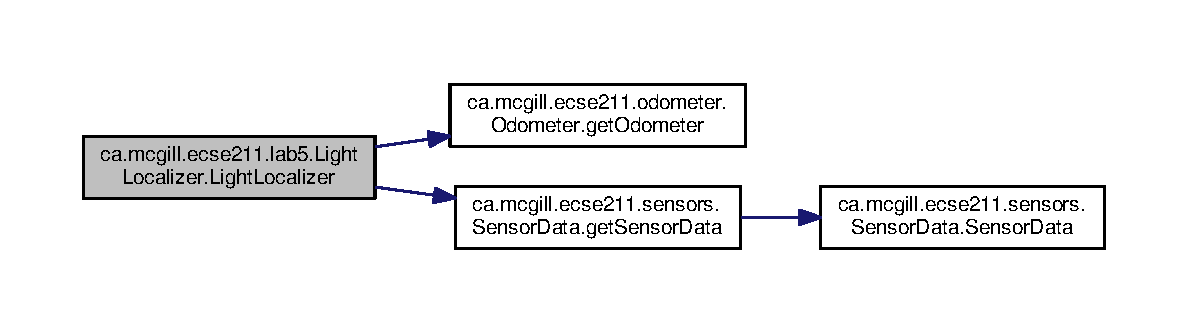
\includegraphics[width=350pt]{classca_1_1mcgill_1_1ecse211_1_1lab5_1_1_light_localizer_a83dbb9eaea19092e27f6f9acdd35d37a_cgraph}
\end{center}
\end{figure}


\subsection{Member Function Documentation}
\mbox{\Hypertarget{classca_1_1mcgill_1_1ecse211_1_1lab5_1_1_light_localizer_ab9d7289c4badf692fd5c83635305f2c5}\label{classca_1_1mcgill_1_1ecse211_1_1lab5_1_1_light_localizer_ab9d7289c4badf692fd5c83635305f2c5}} 
\index{ca\+::mcgill\+::ecse211\+::lab5\+::\+Light\+Localizer@{ca\+::mcgill\+::ecse211\+::lab5\+::\+Light\+Localizer}!convert\+Angle@{convert\+Angle}}
\index{convert\+Angle@{convert\+Angle}!ca\+::mcgill\+::ecse211\+::lab5\+::\+Light\+Localizer@{ca\+::mcgill\+::ecse211\+::lab5\+::\+Light\+Localizer}}
\subsubsection{\texorpdfstring{convert\+Angle()}{convertAngle()}}
{\footnotesize\ttfamily static int ca.\+mcgill.\+ecse211.\+lab5.\+Light\+Localizer.\+convert\+Angle (\begin{DoxyParamCaption}\item[{double}]{radius,  }\item[{double}]{width,  }\item[{double}]{angle }\end{DoxyParamCaption})\hspace{0.3cm}{\ttfamily [static]}}

This method allows the conversion of an angle value


\begin{DoxyParams}{Parameters}
{\em radius} & The radius of our wheels \\
\hline
{\em distance} & The distance travelled \\
\hline
{\em angle} & The angle to convert \\
\hline
\end{DoxyParams}
\begin{DoxyReturn}{Returns}
A converted angle 
\end{DoxyReturn}


Definition at line 103 of file Light\+Localizer.\+java.

Here is the call graph for this function\+:\nopagebreak
\begin{figure}[H]
\begin{center}
\leavevmode
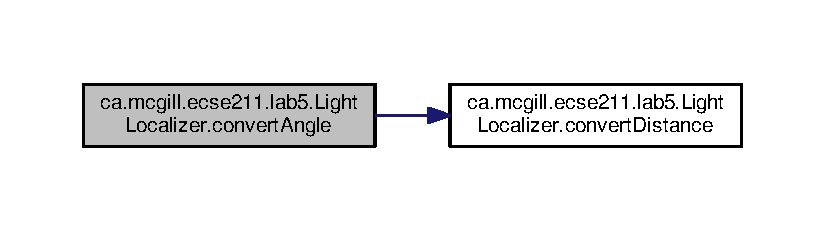
\includegraphics[width=350pt]{classca_1_1mcgill_1_1ecse211_1_1lab5_1_1_light_localizer_ab9d7289c4badf692fd5c83635305f2c5_cgraph}
\end{center}
\end{figure}
\mbox{\Hypertarget{classca_1_1mcgill_1_1ecse211_1_1lab5_1_1_light_localizer_a9eebe889aa2d4d2e881f413cc727cd9c}\label{classca_1_1mcgill_1_1ecse211_1_1lab5_1_1_light_localizer_a9eebe889aa2d4d2e881f413cc727cd9c}} 
\index{ca\+::mcgill\+::ecse211\+::lab5\+::\+Light\+Localizer@{ca\+::mcgill\+::ecse211\+::lab5\+::\+Light\+Localizer}!convert\+Distance@{convert\+Distance}}
\index{convert\+Distance@{convert\+Distance}!ca\+::mcgill\+::ecse211\+::lab5\+::\+Light\+Localizer@{ca\+::mcgill\+::ecse211\+::lab5\+::\+Light\+Localizer}}
\subsubsection{\texorpdfstring{convert\+Distance()}{convertDistance()}}
{\footnotesize\ttfamily static int ca.\+mcgill.\+ecse211.\+lab5.\+Light\+Localizer.\+convert\+Distance (\begin{DoxyParamCaption}\item[{double}]{radius,  }\item[{double}]{distance }\end{DoxyParamCaption})\hspace{0.3cm}{\ttfamily [static]}}

This method allows the conversion of a distance to the total rotation of each wheel need to cover that distance.


\begin{DoxyParams}{Parameters}
{\em radius} & The radius of our wheels \\
\hline
{\em distance} & The distance travelled \\
\hline
\end{DoxyParams}
\begin{DoxyReturn}{Returns}
A converted distance 
\end{DoxyReturn}


Definition at line 91 of file Light\+Localizer.\+java.

Here is the caller graph for this function\+:\nopagebreak
\begin{figure}[H]
\begin{center}
\leavevmode
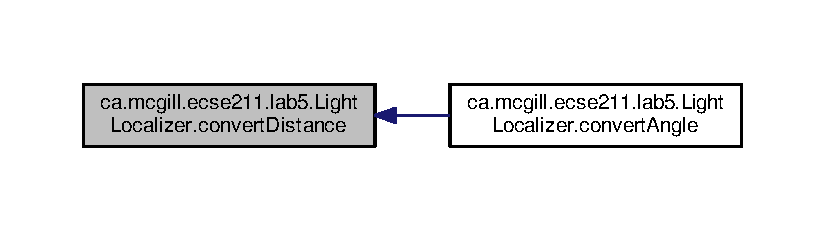
\includegraphics[width=350pt]{classca_1_1mcgill_1_1ecse211_1_1lab5_1_1_light_localizer_a9eebe889aa2d4d2e881f413cc727cd9c_icgraph}
\end{center}
\end{figure}
\mbox{\Hypertarget{classca_1_1mcgill_1_1ecse211_1_1lab5_1_1_light_localizer_a441f56a899fae5bc9c1d6a6d25fbe0bb}\label{classca_1_1mcgill_1_1ecse211_1_1lab5_1_1_light_localizer_a441f56a899fae5bc9c1d6a6d25fbe0bb}} 
\index{ca\+::mcgill\+::ecse211\+::lab5\+::\+Light\+Localizer@{ca\+::mcgill\+::ecse211\+::lab5\+::\+Light\+Localizer}!localize@{localize}}
\index{localize@{localize}!ca\+::mcgill\+::ecse211\+::lab5\+::\+Light\+Localizer@{ca\+::mcgill\+::ecse211\+::lab5\+::\+Light\+Localizer}}
\subsubsection{\texorpdfstring{localize()}{localize()}}
{\footnotesize\ttfamily void ca.\+mcgill.\+ecse211.\+lab5.\+Light\+Localizer.\+localize (\begin{DoxyParamCaption}\item[{int \mbox{[}$\,$\mbox{]}}]{sC }\end{DoxyParamCaption})}

Once the robot know what angle it is facing, this method looks for the x,y axis origins knowing it is in the first tile facing north. 

Definition at line 46 of file Light\+Localizer.\+java.

Here is the call graph for this function\+:\nopagebreak
\begin{figure}[H]
\begin{center}
\leavevmode
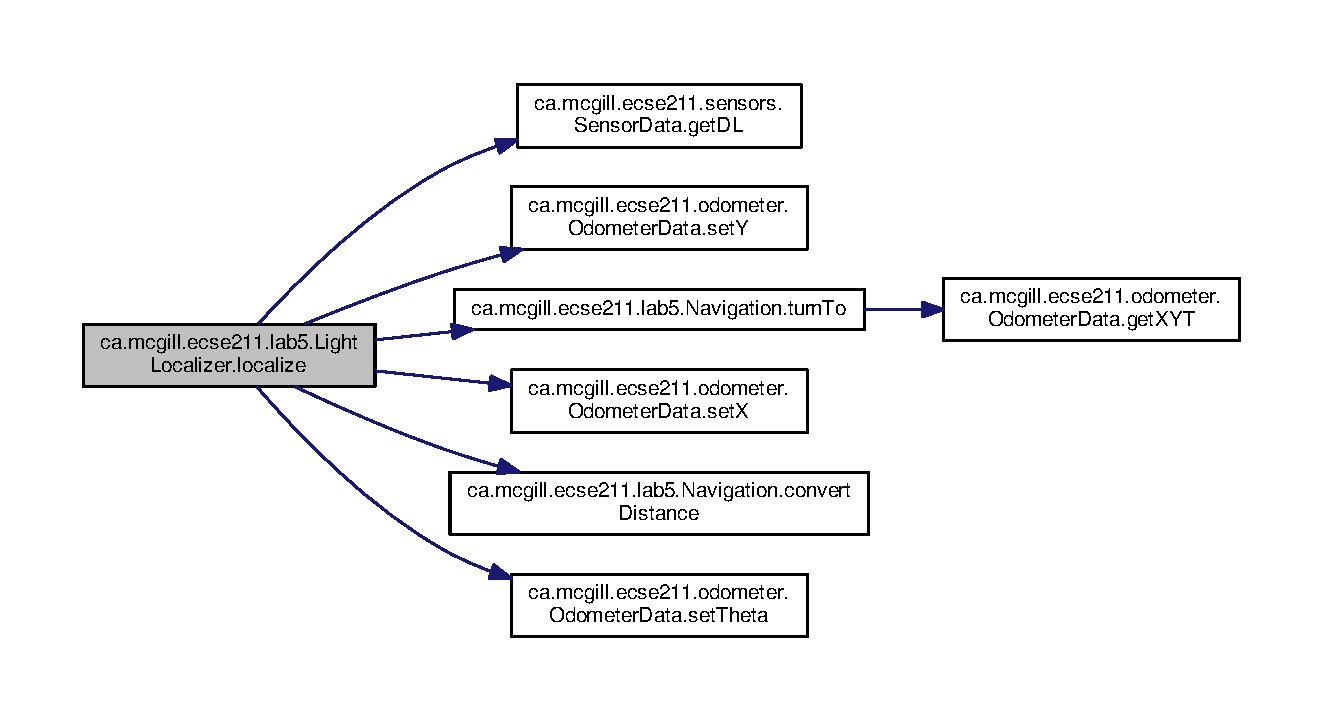
\includegraphics[width=350pt]{classca_1_1mcgill_1_1ecse211_1_1lab5_1_1_light_localizer_a441f56a899fae5bc9c1d6a6d25fbe0bb_cgraph}
\end{center}
\end{figure}


The documentation for this class was generated from the following file\+:\begin{DoxyCompactItemize}
\item 
/home/ccc/\+Eclipse-\/\+Workspace-\/\+Oxygen/\+Lab5-\/\+Search\+And\+Localize/src/ca/mcgill/ecse211/lab5/Light\+Localizer.\+java\end{DoxyCompactItemize}

\hypertarget{classca_1_1mcgill_1_1ecse211_1_1sensors_1_1_light_poller}{}\section{ca.\+mcgill.\+ecse211.\+sensors.\+Light\+Poller Class Reference}
\label{classca_1_1mcgill_1_1ecse211_1_1sensors_1_1_light_poller}\index{ca.\+mcgill.\+ecse211.\+sensors.\+Light\+Poller@{ca.\+mcgill.\+ecse211.\+sensors.\+Light\+Poller}}


Inheritance diagram for ca.\+mcgill.\+ecse211.\+sensors.\+Light\+Poller\+:\nopagebreak
\begin{figure}[H]
\begin{center}
\leavevmode
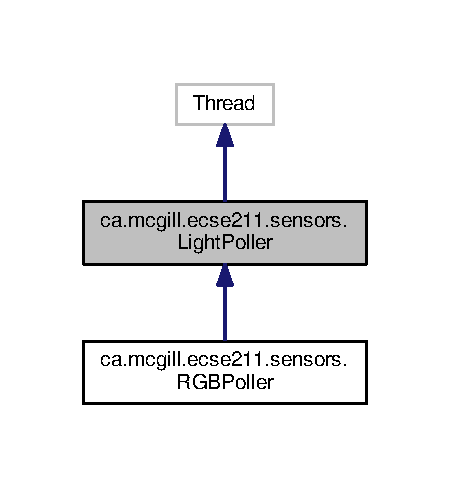
\includegraphics[width=216pt]{classca_1_1mcgill_1_1ecse211_1_1sensors_1_1_light_poller__inherit__graph}
\end{center}
\end{figure}


Collaboration diagram for ca.\+mcgill.\+ecse211.\+sensors.\+Light\+Poller\+:\nopagebreak
\begin{figure}[H]
\begin{center}
\leavevmode
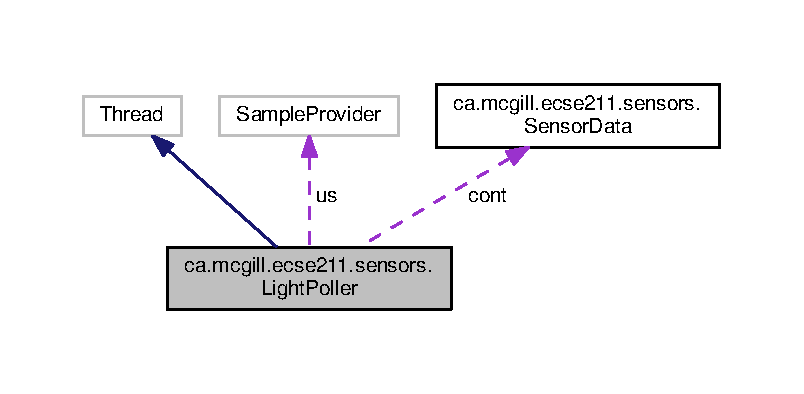
\includegraphics[width=350pt]{classca_1_1mcgill_1_1ecse211_1_1sensors_1_1_light_poller__coll__graph}
\end{center}
\end{figure}
\subsection*{Public Member Functions}
\begin{DoxyCompactItemize}
\item 
\hyperlink{classca_1_1mcgill_1_1ecse211_1_1sensors_1_1_light_poller_aa284d0f6d7e032d3610a7ad428f16132}{Light\+Poller} (Sample\+Provider us, float\mbox{[}$\,$\mbox{]} lg\+Data, \hyperlink{classca_1_1mcgill_1_1ecse211_1_1sensors_1_1_sensor_data}{Sensor\+Data} cont)  throws Odometer\+Exceptions 
\item 
void \hyperlink{classca_1_1mcgill_1_1ecse211_1_1sensors_1_1_light_poller_a31751b40132d9402de493aa9ec11d9d5}{run} ()
\end{DoxyCompactItemize}
\subsection*{Protected Member Functions}
\begin{DoxyCompactItemize}
\item 
\mbox{\Hypertarget{classca_1_1mcgill_1_1ecse211_1_1sensors_1_1_light_poller_af7c5e71f9ef2c6bebd4a67ba6b533f28}\label{classca_1_1mcgill_1_1ecse211_1_1sensors_1_1_light_poller_af7c5e71f9ef2c6bebd4a67ba6b533f28}} 
void {\bfseries process\+Data} ()
\end{DoxyCompactItemize}
\subsection*{Protected Attributes}
\begin{DoxyCompactItemize}
\item 
\mbox{\Hypertarget{classca_1_1mcgill_1_1ecse211_1_1sensors_1_1_light_poller_a697ac7826ad649b453cf9cdd1b5f723b}\label{classca_1_1mcgill_1_1ecse211_1_1sensors_1_1_light_poller_a697ac7826ad649b453cf9cdd1b5f723b}} 
Sample\+Provider {\bfseries us}
\item 
\mbox{\Hypertarget{classca_1_1mcgill_1_1ecse211_1_1sensors_1_1_light_poller_a2c208445d4fb1feedd269c0fda447d6f}\label{classca_1_1mcgill_1_1ecse211_1_1sensors_1_1_light_poller_a2c208445d4fb1feedd269c0fda447d6f}} 
\hyperlink{classca_1_1mcgill_1_1ecse211_1_1sensors_1_1_sensor_data}{Sensor\+Data} {\bfseries cont}
\item 
\mbox{\Hypertarget{classca_1_1mcgill_1_1ecse211_1_1sensors_1_1_light_poller_af014631d513b89ba9a55f0e7d0e8d754}\label{classca_1_1mcgill_1_1ecse211_1_1sensors_1_1_light_poller_af014631d513b89ba9a55f0e7d0e8d754}} 
float \mbox{[}$\,$\mbox{]} {\bfseries lg\+Data}
\end{DoxyCompactItemize}


\subsection{Detailed Description}
This class implements the Light Sensor Poller for our robot

\begin{DoxyAuthor}{Author}
Caspar Cedro \& Percy Chen \& Patrick Erath \& Anssam Ghezala \& Susan Matuszewski \& Kamy Moussavi Kafi 
\end{DoxyAuthor}


Definition at line 12 of file Light\+Poller.\+java.



\subsection{Constructor \& Destructor Documentation}
\mbox{\Hypertarget{classca_1_1mcgill_1_1ecse211_1_1sensors_1_1_light_poller_aa284d0f6d7e032d3610a7ad428f16132}\label{classca_1_1mcgill_1_1ecse211_1_1sensors_1_1_light_poller_aa284d0f6d7e032d3610a7ad428f16132}} 
\index{ca\+::mcgill\+::ecse211\+::sensors\+::\+Light\+Poller@{ca\+::mcgill\+::ecse211\+::sensors\+::\+Light\+Poller}!Light\+Poller@{Light\+Poller}}
\index{Light\+Poller@{Light\+Poller}!ca\+::mcgill\+::ecse211\+::sensors\+::\+Light\+Poller@{ca\+::mcgill\+::ecse211\+::sensors\+::\+Light\+Poller}}
\subsubsection{\texorpdfstring{Light\+Poller()}{LightPoller()}}
{\footnotesize\ttfamily ca.\+mcgill.\+ecse211.\+sensors.\+Light\+Poller.\+Light\+Poller (\begin{DoxyParamCaption}\item[{Sample\+Provider}]{us,  }\item[{float \mbox{[}$\,$\mbox{]}}]{lg\+Data,  }\item[{\hyperlink{classca_1_1mcgill_1_1ecse211_1_1sensors_1_1_sensor_data}{Sensor\+Data}}]{cont }\end{DoxyParamCaption}) throws \hyperlink{classca_1_1mcgill_1_1ecse211_1_1odometer_1_1_odometer_exceptions}{Odometer\+Exceptions}}

This constructor creates an instance of the \hyperlink{classca_1_1mcgill_1_1ecse211_1_1sensors_1_1_light_poller}{Light\+Poller} class to provide distance data from an light sensor to our robot.


\begin{DoxyParams}{Parameters}
{\em us} & a Sample\+Provider class instance that helps us to store an array of ultrasonic sensor data. \\
\hline
{\em lg\+Data} & an array of distance data to be used by our Wall Follower\textquotesingle{}s Ultrasonic\+Controllers. \\
\hline
{\em cont} & a Bang\+Bang\+Controller or P\+Controller instance that has accumulated distance data stored in us\+Data passed to it. \\
\hline
\end{DoxyParams}

\begin{DoxyExceptions}{Exceptions}
{\em Odometer\+Exceptions} & \\
\hline
\end{DoxyExceptions}


Definition at line 29 of file Light\+Poller.\+java.



\subsection{Member Function Documentation}
\mbox{\Hypertarget{classca_1_1mcgill_1_1ecse211_1_1sensors_1_1_light_poller_a31751b40132d9402de493aa9ec11d9d5}\label{classca_1_1mcgill_1_1ecse211_1_1sensors_1_1_light_poller_a31751b40132d9402de493aa9ec11d9d5}} 
\index{ca\+::mcgill\+::ecse211\+::sensors\+::\+Light\+Poller@{ca\+::mcgill\+::ecse211\+::sensors\+::\+Light\+Poller}!run@{run}}
\index{run@{run}!ca\+::mcgill\+::ecse211\+::sensors\+::\+Light\+Poller@{ca\+::mcgill\+::ecse211\+::sensors\+::\+Light\+Poller}}
\subsubsection{\texorpdfstring{run()}{run()}}
{\footnotesize\ttfamily void ca.\+mcgill.\+ecse211.\+sensors.\+Light\+Poller.\+run (\begin{DoxyParamCaption}{ }\end{DoxyParamCaption})}

This method is called by a \hyperlink{classca_1_1mcgill_1_1ecse211_1_1sensors_1_1_ultrasonic_poller}{Ultrasonic\+Poller} (Thread) instance when it is asked to start executing

Sensors now return floats using a uniform protocol. Need to convert US result to an integer \mbox{[}0,255\mbox{]} (non-\/\+Javadoc)

\begin{DoxySeeAlso}{See also}
java.\+lang.\+Thread\+::run() 
\end{DoxySeeAlso}


Definition at line 44 of file Light\+Poller.\+java.

Here is the call graph for this function\+:\nopagebreak
\begin{figure}[H]
\begin{center}
\leavevmode
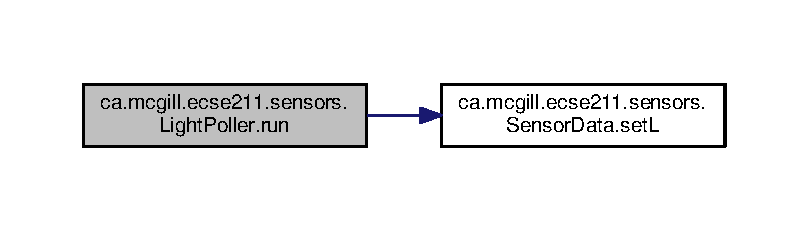
\includegraphics[width=350pt]{classca_1_1mcgill_1_1ecse211_1_1sensors_1_1_light_poller_a31751b40132d9402de493aa9ec11d9d5_cgraph}
\end{center}
\end{figure}


The documentation for this class was generated from the following file\+:\begin{DoxyCompactItemize}
\item 
/home/ccc/\+Eclipse-\/\+Workspace-\/\+Oxygen/\+Lab5-\/\+Search\+And\+Localize/src/ca/mcgill/ecse211/sensors/Light\+Poller.\+java\end{DoxyCompactItemize}

\hypertarget{classca_1_1mcgill_1_1ecse211_1_1lab5_1_1_navigation}{}\section{ca.\+mcgill.\+ecse211.\+lab5.\+Navigation Class Reference}
\label{classca_1_1mcgill_1_1ecse211_1_1lab5_1_1_navigation}\index{ca.\+mcgill.\+ecse211.\+lab5.\+Navigation@{ca.\+mcgill.\+ecse211.\+lab5.\+Navigation}}
\subsection*{Public Member Functions}
\begin{DoxyCompactItemize}
\item 
\hyperlink{classca_1_1mcgill_1_1ecse211_1_1lab5_1_1_navigation_a93b746f61226c3b14532c43d0c2f61dd}{Navigation} (E\+V3\+Large\+Regulated\+Motor left\+Motor, E\+V3\+Large\+Regulated\+Motor right\+Motor)  throws Odometer\+Exceptions 
\item 
void \hyperlink{classca_1_1mcgill_1_1ecse211_1_1lab5_1_1_navigation_a318969f4776d0bf4a8721be3d2444a5c}{travel\+To} (double x, double y, boolean \hyperlink{classca_1_1mcgill_1_1ecse211_1_1lab5_1_1_navigation_a73a89ddd822e0ba1cfd7a29c18aa7aea}{do\+Correction})
\item 
\mbox{\Hypertarget{classca_1_1mcgill_1_1ecse211_1_1lab5_1_1_navigation_aacb83ee18419dcd6095e331975cf2167}\label{classca_1_1mcgill_1_1ecse211_1_1lab5_1_1_navigation_aacb83ee18419dcd6095e331975cf2167}} 
void {\bfseries travel\+Back\+To} (double x, double y)
\item 
void \hyperlink{classca_1_1mcgill_1_1ecse211_1_1lab5_1_1_navigation_a2b39928c8062fe6863de8e818d009e91}{turn\+To} (double angle, boolean async)
\item 
void \hyperlink{classca_1_1mcgill_1_1ecse211_1_1lab5_1_1_navigation_a73a89ddd822e0ba1cfd7a29c18aa7aea}{do\+Correction} (double angle)
\item 
void \hyperlink{classca_1_1mcgill_1_1ecse211_1_1lab5_1_1_navigation_a5fcce0063a6b557d349a6fb5bf144c64}{rotate} (int angle)
\item 
void \hyperlink{classca_1_1mcgill_1_1ecse211_1_1lab5_1_1_navigation_afe038af6692e7ad28c3587cd979d7223}{stop} ()
\end{DoxyCompactItemize}
\subsection*{Static Public Member Functions}
\begin{DoxyCompactItemize}
\item 
static int \hyperlink{classca_1_1mcgill_1_1ecse211_1_1lab5_1_1_navigation_a85122ad723d0988c118866f367073be6}{convert\+Distance} (double radius, double distance)
\end{DoxyCompactItemize}


\subsection{Detailed Description}
The Navigator class extends the functionality of the \hyperlink{classca_1_1mcgill_1_1ecse211_1_1lab5_1_1_navigation}{Navigation} class. It offers an alternative \hyperlink{classca_1_1mcgill_1_1ecse211_1_1lab5_1_1_navigation_a318969f4776d0bf4a8721be3d2444a5c}{travel\+To()} method which uses a state machine to implement obstacle avoidance.

The Navigator class does not override any of the methods in \hyperlink{classca_1_1mcgill_1_1ecse211_1_1lab5_1_1_navigation}{Navigation}. All methods with the same name are overloaded i.\+e. the Navigator version takes different parameters than the \hyperlink{classca_1_1mcgill_1_1ecse211_1_1lab5_1_1_navigation}{Navigation} version.

This is useful if, for instance, you want to force travel without obstacle detection over small distances. One place where you might want to do this is in the Obstacle\+Avoidance class. Another place is methods that implement specific features for future milestones such as retrieving an object.

\begin{DoxyAuthor}{Author}
Caspar Cedro \& Percy Chen \& Patrick Erath \& Anssam Ghezala \& Susan Matuszewski \& Kamy Moussavi Kafi 
\end{DoxyAuthor}


Definition at line 25 of file Navigation.\+java.



\subsection{Constructor \& Destructor Documentation}
\mbox{\Hypertarget{classca_1_1mcgill_1_1ecse211_1_1lab5_1_1_navigation_a93b746f61226c3b14532c43d0c2f61dd}\label{classca_1_1mcgill_1_1ecse211_1_1lab5_1_1_navigation_a93b746f61226c3b14532c43d0c2f61dd}} 
\index{ca\+::mcgill\+::ecse211\+::lab5\+::\+Navigation@{ca\+::mcgill\+::ecse211\+::lab5\+::\+Navigation}!Navigation@{Navigation}}
\index{Navigation@{Navigation}!ca\+::mcgill\+::ecse211\+::lab5\+::\+Navigation@{ca\+::mcgill\+::ecse211\+::lab5\+::\+Navigation}}
\subsubsection{\texorpdfstring{Navigation()}{Navigation()}}
{\footnotesize\ttfamily ca.\+mcgill.\+ecse211.\+lab5.\+Navigation.\+Navigation (\begin{DoxyParamCaption}\item[{E\+V3\+Large\+Regulated\+Motor}]{left\+Motor,  }\item[{E\+V3\+Large\+Regulated\+Motor}]{right\+Motor }\end{DoxyParamCaption}) throws \hyperlink{classca_1_1mcgill_1_1ecse211_1_1odometer_1_1_odometer_exceptions}{Odometer\+Exceptions}}

This navigation class constructor sets up our robot to begin navigating a particular map


\begin{DoxyParams}{Parameters}
{\em left\+Motor} & The E\+V3\+Large\+Regulated\+Motor instance for our left motor \\
\hline
{\em right\+Motor} & The E\+V3\+Large\+Regulated\+Motor instance for our right motor \\
\hline
\end{DoxyParams}


Definition at line 41 of file Navigation.\+java.

Here is the call graph for this function\+:
\nopagebreak
\begin{figure}[H]
\begin{center}
\leavevmode
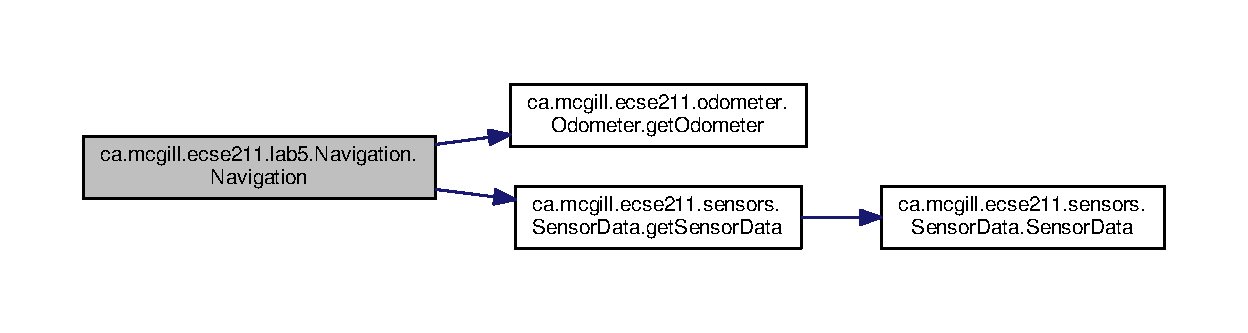
\includegraphics[width=350pt]{classca_1_1mcgill_1_1ecse211_1_1lab5_1_1_navigation_a93b746f61226c3b14532c43d0c2f61dd_cgraph}
\end{center}
\end{figure}


\subsection{Member Function Documentation}
\mbox{\Hypertarget{classca_1_1mcgill_1_1ecse211_1_1lab5_1_1_navigation_a85122ad723d0988c118866f367073be6}\label{classca_1_1mcgill_1_1ecse211_1_1lab5_1_1_navigation_a85122ad723d0988c118866f367073be6}} 
\index{ca\+::mcgill\+::ecse211\+::lab5\+::\+Navigation@{ca\+::mcgill\+::ecse211\+::lab5\+::\+Navigation}!convert\+Distance@{convert\+Distance}}
\index{convert\+Distance@{convert\+Distance}!ca\+::mcgill\+::ecse211\+::lab5\+::\+Navigation@{ca\+::mcgill\+::ecse211\+::lab5\+::\+Navigation}}
\subsubsection{\texorpdfstring{convert\+Distance()}{convertDistance()}}
{\footnotesize\ttfamily static int ca.\+mcgill.\+ecse211.\+lab5.\+Navigation.\+convert\+Distance (\begin{DoxyParamCaption}\item[{double}]{radius,  }\item[{double}]{distance }\end{DoxyParamCaption})\hspace{0.3cm}{\ttfamily [static]}}

This method allows the conversion of a distance to the total rotation of each wheel need to cover that distance.


\begin{DoxyParams}{Parameters}
{\em radius} & The radius of our wheels \\
\hline
{\em distance} & The distance travelled \\
\hline
\end{DoxyParams}
\begin{DoxyReturn}{Returns}
A converted distance 
\end{DoxyReturn}


Definition at line 181 of file Navigation.\+java.

Here is the caller graph for this function\+:
\nopagebreak
\begin{figure}[H]
\begin{center}
\leavevmode
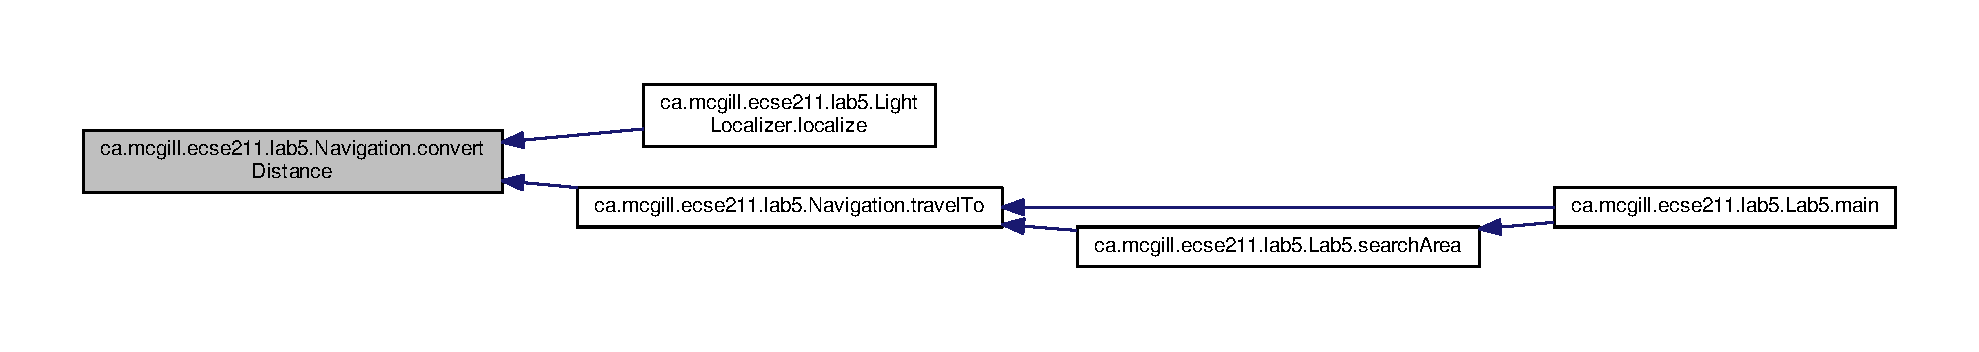
\includegraphics[width=350pt]{classca_1_1mcgill_1_1ecse211_1_1lab5_1_1_navigation_a85122ad723d0988c118866f367073be6_icgraph}
\end{center}
\end{figure}
\mbox{\Hypertarget{classca_1_1mcgill_1_1ecse211_1_1lab5_1_1_navigation_a73a89ddd822e0ba1cfd7a29c18aa7aea}\label{classca_1_1mcgill_1_1ecse211_1_1lab5_1_1_navigation_a73a89ddd822e0ba1cfd7a29c18aa7aea}} 
\index{ca\+::mcgill\+::ecse211\+::lab5\+::\+Navigation@{ca\+::mcgill\+::ecse211\+::lab5\+::\+Navigation}!do\+Correction@{do\+Correction}}
\index{do\+Correction@{do\+Correction}!ca\+::mcgill\+::ecse211\+::lab5\+::\+Navigation@{ca\+::mcgill\+::ecse211\+::lab5\+::\+Navigation}}
\subsubsection{\texorpdfstring{do\+Correction()}{doCorrection()}}
{\footnotesize\ttfamily void ca.\+mcgill.\+ecse211.\+lab5.\+Navigation.\+do\+Correction (\begin{DoxyParamCaption}\item[{double}]{angle }\end{DoxyParamCaption})}


\begin{DoxyParams}{Parameters}
{\em angle} & \\
\hline
\end{DoxyParams}


Definition at line 141 of file Navigation.\+java.

Here is the call graph for this function\+:
\nopagebreak
\begin{figure}[H]
\begin{center}
\leavevmode
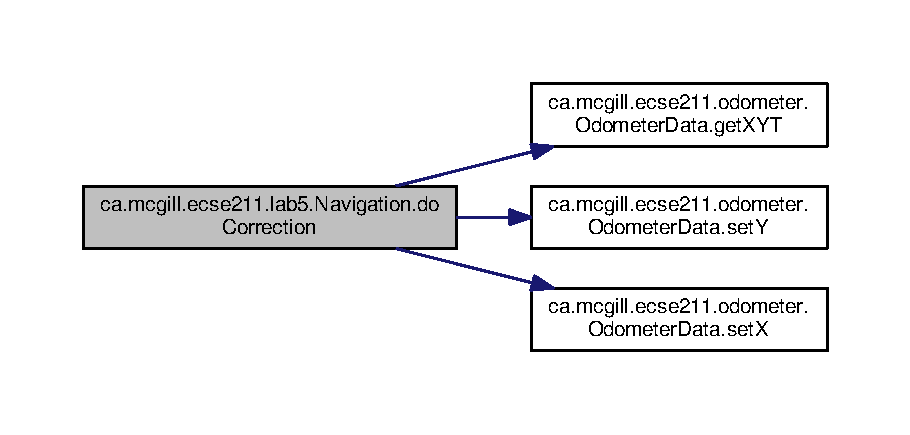
\includegraphics[width=350pt]{classca_1_1mcgill_1_1ecse211_1_1lab5_1_1_navigation_a73a89ddd822e0ba1cfd7a29c18aa7aea_cgraph}
\end{center}
\end{figure}
Here is the caller graph for this function\+:
\nopagebreak
\begin{figure}[H]
\begin{center}
\leavevmode
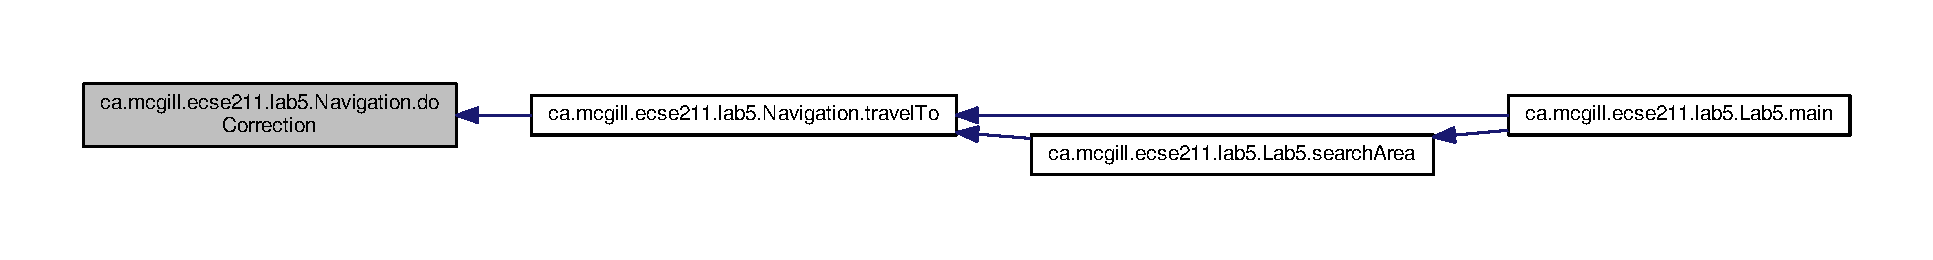
\includegraphics[width=350pt]{classca_1_1mcgill_1_1ecse211_1_1lab5_1_1_navigation_a73a89ddd822e0ba1cfd7a29c18aa7aea_icgraph}
\end{center}
\end{figure}
\mbox{\Hypertarget{classca_1_1mcgill_1_1ecse211_1_1lab5_1_1_navigation_a5fcce0063a6b557d349a6fb5bf144c64}\label{classca_1_1mcgill_1_1ecse211_1_1lab5_1_1_navigation_a5fcce0063a6b557d349a6fb5bf144c64}} 
\index{ca\+::mcgill\+::ecse211\+::lab5\+::\+Navigation@{ca\+::mcgill\+::ecse211\+::lab5\+::\+Navigation}!rotate@{rotate}}
\index{rotate@{rotate}!ca\+::mcgill\+::ecse211\+::lab5\+::\+Navigation@{ca\+::mcgill\+::ecse211\+::lab5\+::\+Navigation}}
\subsubsection{\texorpdfstring{rotate()}{rotate()}}
{\footnotesize\ttfamily void ca.\+mcgill.\+ecse211.\+lab5.\+Navigation.\+rotate (\begin{DoxyParamCaption}\item[{int}]{angle }\end{DoxyParamCaption})}

Rotate the robot by certain angle


\begin{DoxyParams}{Parameters}
{\em angle} & \\
\hline
\end{DoxyParams}


Definition at line 160 of file Navigation.\+java.

\mbox{\Hypertarget{classca_1_1mcgill_1_1ecse211_1_1lab5_1_1_navigation_afe038af6692e7ad28c3587cd979d7223}\label{classca_1_1mcgill_1_1ecse211_1_1lab5_1_1_navigation_afe038af6692e7ad28c3587cd979d7223}} 
\index{ca\+::mcgill\+::ecse211\+::lab5\+::\+Navigation@{ca\+::mcgill\+::ecse211\+::lab5\+::\+Navigation}!stop@{stop}}
\index{stop@{stop}!ca\+::mcgill\+::ecse211\+::lab5\+::\+Navigation@{ca\+::mcgill\+::ecse211\+::lab5\+::\+Navigation}}
\subsubsection{\texorpdfstring{stop()}{stop()}}
{\footnotesize\ttfamily void ca.\+mcgill.\+ecse211.\+lab5.\+Navigation.\+stop (\begin{DoxyParamCaption}{ }\end{DoxyParamCaption})}

Stop the motor 

Definition at line 168 of file Navigation.\+java.

Here is the caller graph for this function\+:
\nopagebreak
\begin{figure}[H]
\begin{center}
\leavevmode
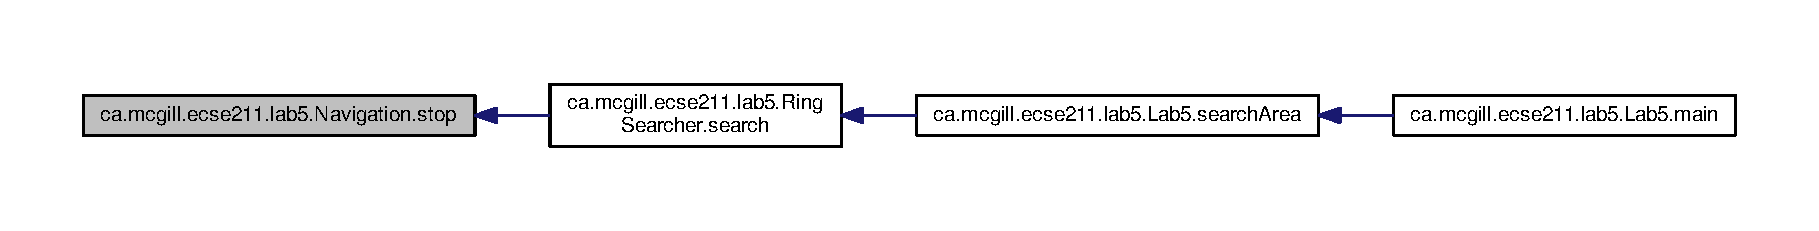
\includegraphics[width=350pt]{classca_1_1mcgill_1_1ecse211_1_1lab5_1_1_navigation_afe038af6692e7ad28c3587cd979d7223_icgraph}
\end{center}
\end{figure}
\mbox{\Hypertarget{classca_1_1mcgill_1_1ecse211_1_1lab5_1_1_navigation_a318969f4776d0bf4a8721be3d2444a5c}\label{classca_1_1mcgill_1_1ecse211_1_1lab5_1_1_navigation_a318969f4776d0bf4a8721be3d2444a5c}} 
\index{ca\+::mcgill\+::ecse211\+::lab5\+::\+Navigation@{ca\+::mcgill\+::ecse211\+::lab5\+::\+Navigation}!travel\+To@{travel\+To}}
\index{travel\+To@{travel\+To}!ca\+::mcgill\+::ecse211\+::lab5\+::\+Navigation@{ca\+::mcgill\+::ecse211\+::lab5\+::\+Navigation}}
\subsubsection{\texorpdfstring{travel\+To()}{travelTo()}}
{\footnotesize\ttfamily void ca.\+mcgill.\+ecse211.\+lab5.\+Navigation.\+travel\+To (\begin{DoxyParamCaption}\item[{double}]{x,  }\item[{double}]{y,  }\item[{boolean}]{do\+Correction }\end{DoxyParamCaption})}

Travel\+To function which takes as arguments the x and y position in cm Will travel to designated position, while constantly updating it\textquotesingle{}s heading

When avoid=true, the nav thread will handle traveling. If you want to travel without avoidance, this is also possible. In this case, the method in the \hyperlink{classca_1_1mcgill_1_1ecse211_1_1lab5_1_1_navigation}{Navigation} class is used.


\begin{DoxyParams}{Parameters}
{\em x} & The x coordinate to travel to (in cm) \\
\hline
{\em y} & The y coordinate to travel to (in cm) \\
\hline
\end{DoxyParams}


Definition at line 64 of file Navigation.\+java.

Here is the call graph for this function\+:
\nopagebreak
\begin{figure}[H]
\begin{center}
\leavevmode
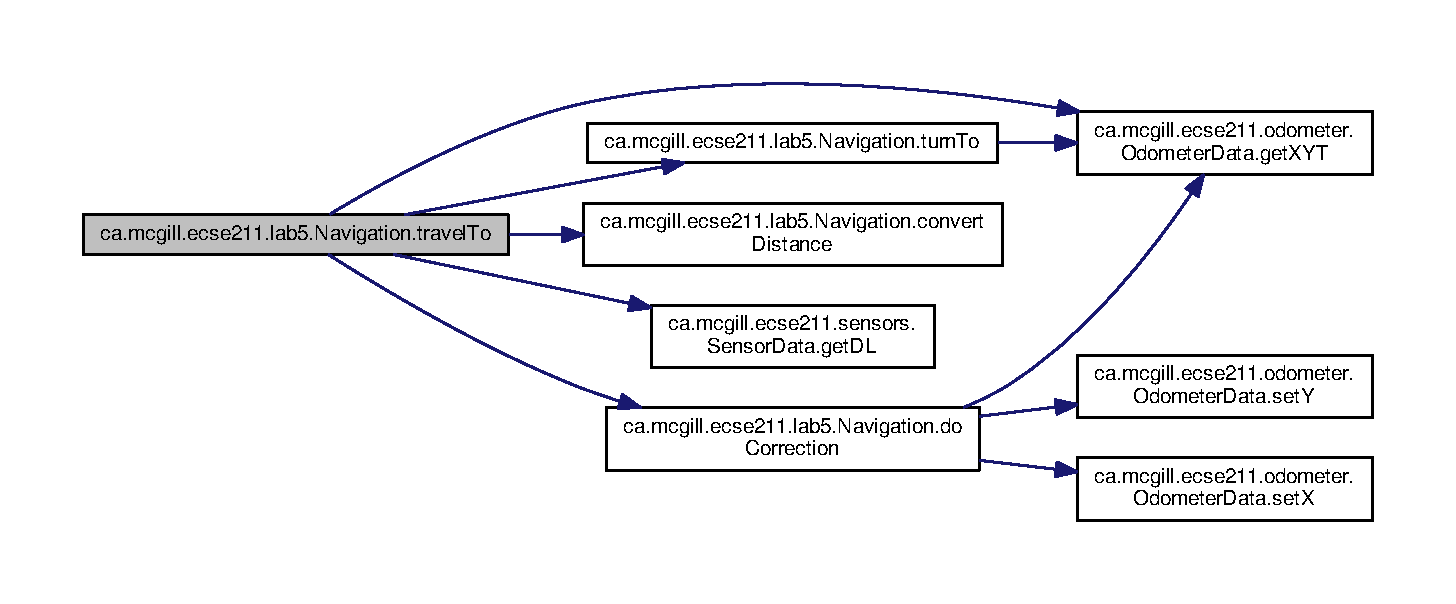
\includegraphics[width=350pt]{classca_1_1mcgill_1_1ecse211_1_1lab5_1_1_navigation_a318969f4776d0bf4a8721be3d2444a5c_cgraph}
\end{center}
\end{figure}
Here is the caller graph for this function\+:
\nopagebreak
\begin{figure}[H]
\begin{center}
\leavevmode
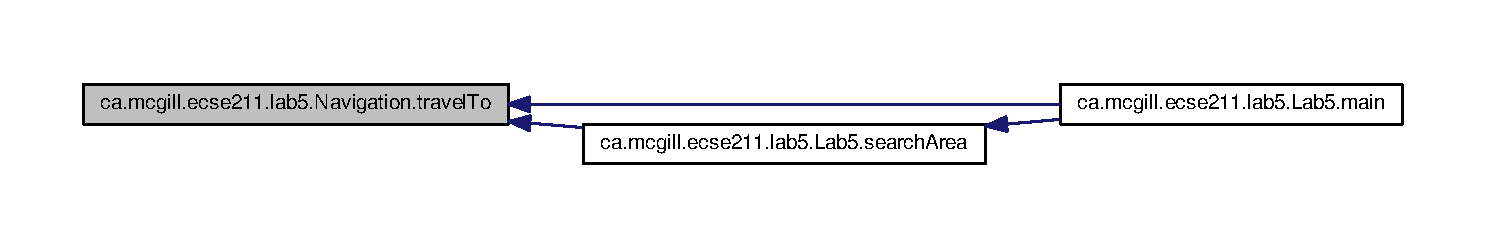
\includegraphics[width=350pt]{classca_1_1mcgill_1_1ecse211_1_1lab5_1_1_navigation_a318969f4776d0bf4a8721be3d2444a5c_icgraph}
\end{center}
\end{figure}
\mbox{\Hypertarget{classca_1_1mcgill_1_1ecse211_1_1lab5_1_1_navigation_a2b39928c8062fe6863de8e818d009e91}\label{classca_1_1mcgill_1_1ecse211_1_1lab5_1_1_navigation_a2b39928c8062fe6863de8e818d009e91}} 
\index{ca\+::mcgill\+::ecse211\+::lab5\+::\+Navigation@{ca\+::mcgill\+::ecse211\+::lab5\+::\+Navigation}!turn\+To@{turn\+To}}
\index{turn\+To@{turn\+To}!ca\+::mcgill\+::ecse211\+::lab5\+::\+Navigation@{ca\+::mcgill\+::ecse211\+::lab5\+::\+Navigation}}
\subsubsection{\texorpdfstring{turn\+To()}{turnTo()}}
{\footnotesize\ttfamily void ca.\+mcgill.\+ecse211.\+lab5.\+Navigation.\+turn\+To (\begin{DoxyParamCaption}\item[{double}]{angle,  }\item[{boolean}]{async }\end{DoxyParamCaption})}

This method is where the logic for the odometer will run. Use the methods provided from the Odometer\+Data class to implement the odometer.


\begin{DoxyParams}{Parameters}
{\em angle} & The angle we want our robot to turn to (in degrees) \\
\hline
\end{DoxyParams}


Definition at line 114 of file Navigation.\+java.

Here is the call graph for this function\+:
\nopagebreak
\begin{figure}[H]
\begin{center}
\leavevmode
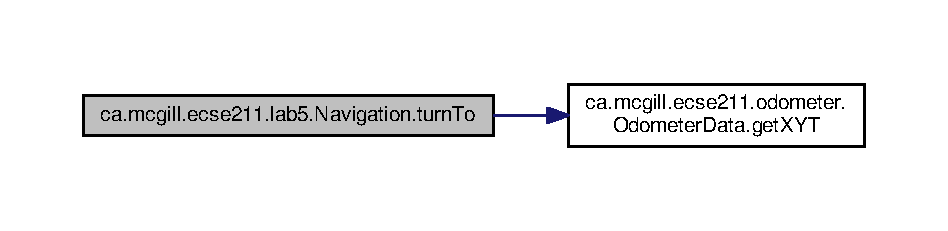
\includegraphics[width=350pt]{classca_1_1mcgill_1_1ecse211_1_1lab5_1_1_navigation_a2b39928c8062fe6863de8e818d009e91_cgraph}
\end{center}
\end{figure}
Here is the caller graph for this function\+:
\nopagebreak
\begin{figure}[H]
\begin{center}
\leavevmode
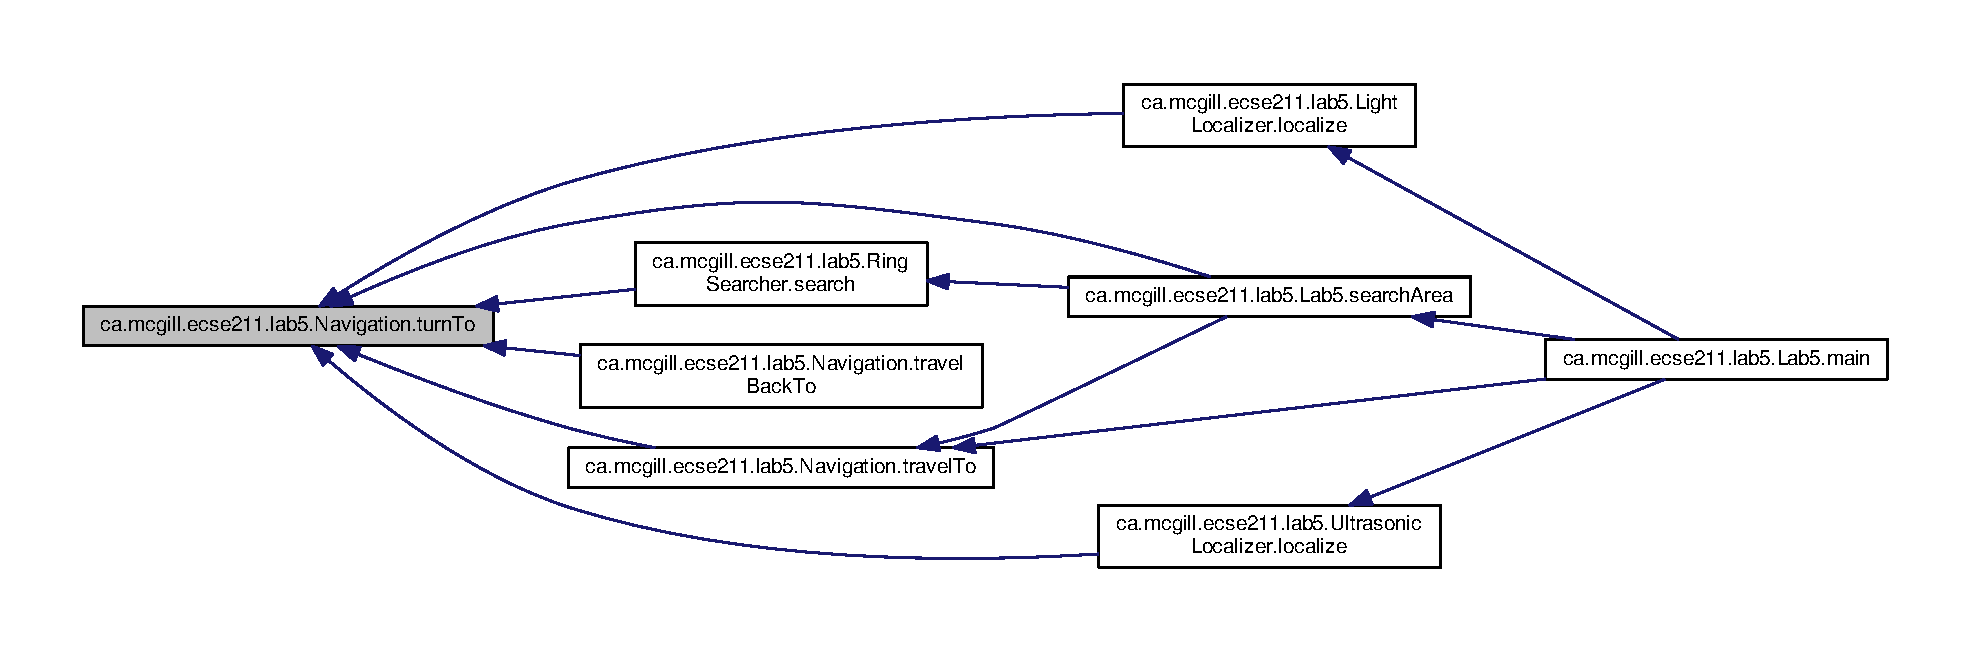
\includegraphics[width=350pt]{classca_1_1mcgill_1_1ecse211_1_1lab5_1_1_navigation_a2b39928c8062fe6863de8e818d009e91_icgraph}
\end{center}
\end{figure}


The documentation for this class was generated from the following file\+:\begin{DoxyCompactItemize}
\item 
/home/ccc/\+Eclipse-\/\+Workspace-\/\+Oxygen/\+Lab5-\/\+Search\+And\+Localize/src/ca/mcgill/ecse211/lab5/Navigation.\+java\end{DoxyCompactItemize}

\hypertarget{classca_1_1mcgill_1_1ecse211_1_1odometer_1_1_odometer}{}\section{ca.\+mcgill.\+ecse211.\+odometer.\+Odometer Class Reference}
\label{classca_1_1mcgill_1_1ecse211_1_1odometer_1_1_odometer}\index{ca.\+mcgill.\+ecse211.\+odometer.\+Odometer@{ca.\+mcgill.\+ecse211.\+odometer.\+Odometer}}


Inheritance diagram for ca.\+mcgill.\+ecse211.\+odometer.\+Odometer\+:
\nopagebreak
\begin{figure}[H]
\begin{center}
\leavevmode
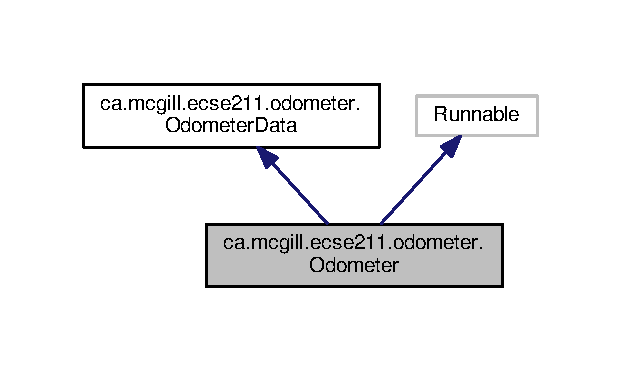
\includegraphics[width=298pt]{classca_1_1mcgill_1_1ecse211_1_1odometer_1_1_odometer__inherit__graph}
\end{center}
\end{figure}


Collaboration diagram for ca.\+mcgill.\+ecse211.\+odometer.\+Odometer\+:
\nopagebreak
\begin{figure}[H]
\begin{center}
\leavevmode
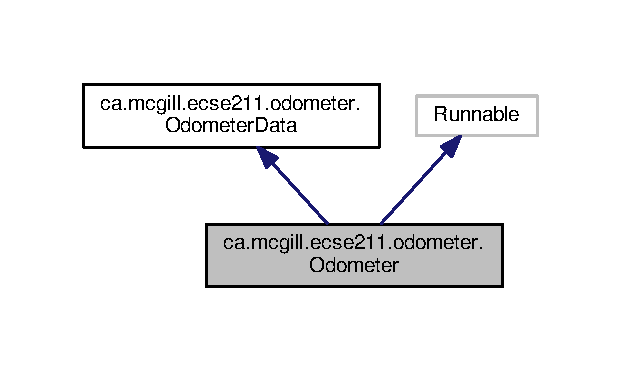
\includegraphics[width=298pt]{classca_1_1mcgill_1_1ecse211_1_1odometer_1_1_odometer__coll__graph}
\end{center}
\end{figure}
\subsection*{Public Member Functions}
\begin{DoxyCompactItemize}
\item 
void \hyperlink{classca_1_1mcgill_1_1ecse211_1_1odometer_1_1_odometer_af0ff4c5121973a8310cf986e25fa0d87}{run} ()
\end{DoxyCompactItemize}
\subsection*{Static Public Member Functions}
\begin{DoxyCompactItemize}
\item 
static synchronized \hyperlink{classca_1_1mcgill_1_1ecse211_1_1odometer_1_1_odometer}{Odometer} \hyperlink{classca_1_1mcgill_1_1ecse211_1_1odometer_1_1_odometer_a99171f11e34dea918fa9dd069d721439}{get\+Odometer} (E\+V3\+Large\+Regulated\+Motor left\+Motor, E\+V3\+Large\+Regulated\+Motor right\+Motor, final double T\+R\+A\+CK, final double W\+H\+E\+E\+L\+\_\+\+R\+AD)  throws Odometer\+Exceptions 
\item 
static synchronized \hyperlink{classca_1_1mcgill_1_1ecse211_1_1odometer_1_1_odometer}{Odometer} \hyperlink{classca_1_1mcgill_1_1ecse211_1_1odometer_1_1_odometer_a4e069b5a96cd43b29af0785244a99b51}{get\+Odometer} ()  throws Odometer\+Exceptions 
\end{DoxyCompactItemize}
\subsection*{Additional Inherited Members}


\subsection{Detailed Description}
This class implements odometry on our robot.

\begin{DoxyAuthor}{Author}
Caspar Cedro 

Percy Chen 

Patrick Erath 

Anssam Ghezala 

Susan Matuszewski 

Kamy Moussavi Kafi 
\end{DoxyAuthor}


Definition at line 26 of file Odometer.\+java.



\subsection{Member Function Documentation}
\mbox{\Hypertarget{classca_1_1mcgill_1_1ecse211_1_1odometer_1_1_odometer_a99171f11e34dea918fa9dd069d721439}\label{classca_1_1mcgill_1_1ecse211_1_1odometer_1_1_odometer_a99171f11e34dea918fa9dd069d721439}} 
\index{ca\+::mcgill\+::ecse211\+::odometer\+::\+Odometer@{ca\+::mcgill\+::ecse211\+::odometer\+::\+Odometer}!get\+Odometer@{get\+Odometer}}
\index{get\+Odometer@{get\+Odometer}!ca\+::mcgill\+::ecse211\+::odometer\+::\+Odometer@{ca\+::mcgill\+::ecse211\+::odometer\+::\+Odometer}}
\subsubsection{\texorpdfstring{get\+Odometer()}{getOdometer()}\hspace{0.1cm}{\footnotesize\ttfamily [1/2]}}
{\footnotesize\ttfamily static synchronized \hyperlink{classca_1_1mcgill_1_1ecse211_1_1odometer_1_1_odometer}{Odometer} ca.\+mcgill.\+ecse211.\+odometer.\+Odometer.\+get\+Odometer (\begin{DoxyParamCaption}\item[{E\+V3\+Large\+Regulated\+Motor}]{left\+Motor,  }\item[{E\+V3\+Large\+Regulated\+Motor}]{right\+Motor,  }\item[{final double}]{T\+R\+A\+CK,  }\item[{final double}]{W\+H\+E\+E\+L\+\_\+\+R\+AD }\end{DoxyParamCaption}) throws \hyperlink{classca_1_1mcgill_1_1ecse211_1_1odometer_1_1_odometer_exceptions}{Odometer\+Exceptions}\hspace{0.3cm}{\ttfamily [static]}}

This method is meant to ensure only one instance of the odometer is used throughout the code.


\begin{DoxyParams}{Parameters}
{\em left\+Motor} & The E\+V3\+Large\+Regulated\+Motor instance for our left motor \\
\hline
{\em right\+Motor} & The E\+V3\+Large\+Regulated\+Motor instance for our right motor \\
\hline
\end{DoxyParams}
\begin{DoxyReturn}{Returns}
new or existing \hyperlink{classca_1_1mcgill_1_1ecse211_1_1odometer_1_1_odometer}{Odometer} Object 
\end{DoxyReturn}

\begin{DoxyExceptions}{Exceptions}
{\em \hyperlink{classca_1_1mcgill_1_1ecse211_1_1odometer_1_1_odometer_exceptions}{Odometer\+Exceptions}} & \\
\hline
\end{DoxyExceptions}


Definition at line 79 of file Odometer.\+java.

Here is the caller graph for this function\+:
\nopagebreak
\begin{figure}[H]
\begin{center}
\leavevmode
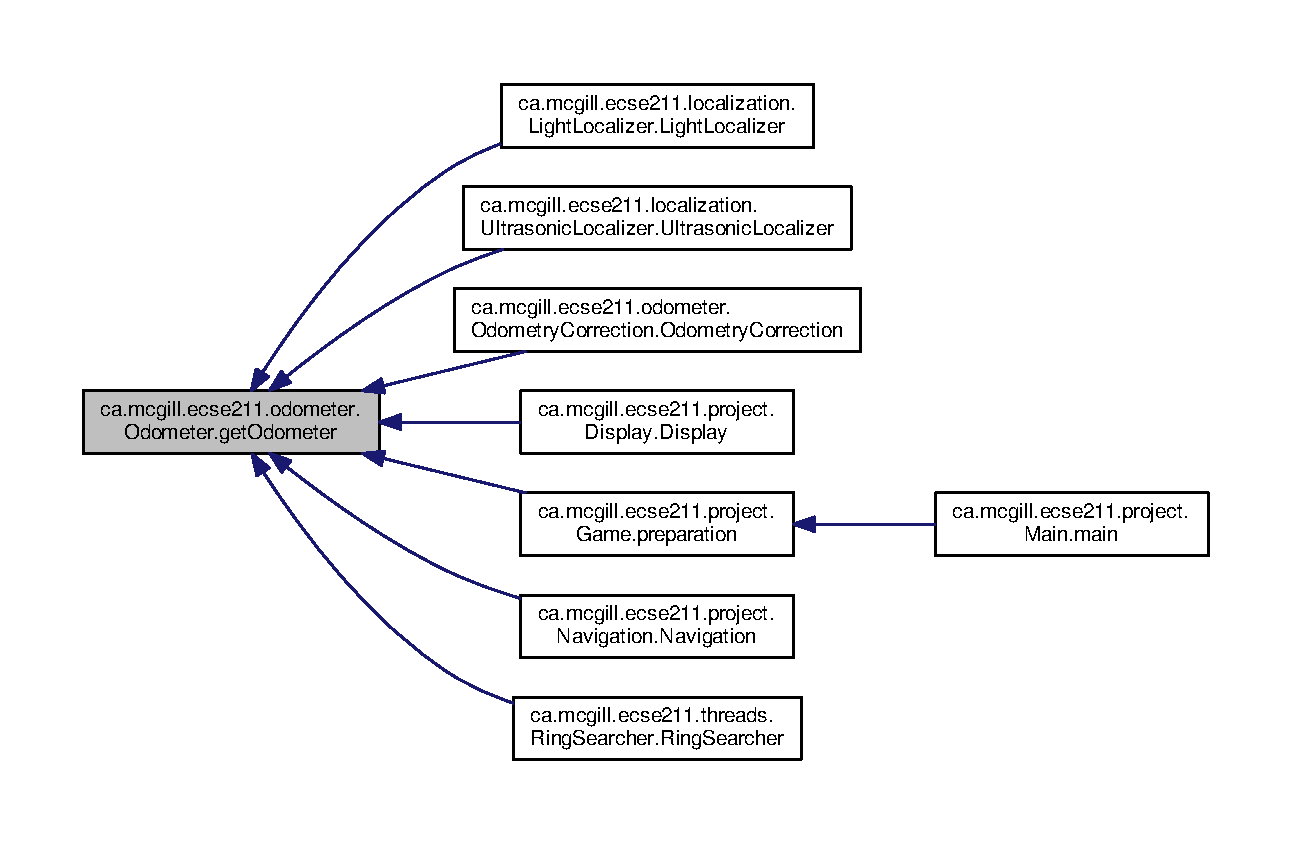
\includegraphics[width=350pt]{classca_1_1mcgill_1_1ecse211_1_1odometer_1_1_odometer_a99171f11e34dea918fa9dd069d721439_icgraph}
\end{center}
\end{figure}
\mbox{\Hypertarget{classca_1_1mcgill_1_1ecse211_1_1odometer_1_1_odometer_a4e069b5a96cd43b29af0785244a99b51}\label{classca_1_1mcgill_1_1ecse211_1_1odometer_1_1_odometer_a4e069b5a96cd43b29af0785244a99b51}} 
\index{ca\+::mcgill\+::ecse211\+::odometer\+::\+Odometer@{ca\+::mcgill\+::ecse211\+::odometer\+::\+Odometer}!get\+Odometer@{get\+Odometer}}
\index{get\+Odometer@{get\+Odometer}!ca\+::mcgill\+::ecse211\+::odometer\+::\+Odometer@{ca\+::mcgill\+::ecse211\+::odometer\+::\+Odometer}}
\subsubsection{\texorpdfstring{get\+Odometer()}{getOdometer()}\hspace{0.1cm}{\footnotesize\ttfamily [2/2]}}
{\footnotesize\ttfamily static synchronized \hyperlink{classca_1_1mcgill_1_1ecse211_1_1odometer_1_1_odometer}{Odometer} ca.\+mcgill.\+ecse211.\+odometer.\+Odometer.\+get\+Odometer (\begin{DoxyParamCaption}{ }\end{DoxyParamCaption}) throws \hyperlink{classca_1_1mcgill_1_1ecse211_1_1odometer_1_1_odometer_exceptions}{Odometer\+Exceptions}\hspace{0.3cm}{\ttfamily [static]}}

This class is meant to return the existing \hyperlink{classca_1_1mcgill_1_1ecse211_1_1odometer_1_1_odometer}{Odometer} Object. It is meant to be used only if an odometer object has been created

\begin{DoxyReturn}{Returns}
error if no previous odometer exists 
\end{DoxyReturn}


Definition at line 96 of file Odometer.\+java.

\mbox{\Hypertarget{classca_1_1mcgill_1_1ecse211_1_1odometer_1_1_odometer_af0ff4c5121973a8310cf986e25fa0d87}\label{classca_1_1mcgill_1_1ecse211_1_1odometer_1_1_odometer_af0ff4c5121973a8310cf986e25fa0d87}} 
\index{ca\+::mcgill\+::ecse211\+::odometer\+::\+Odometer@{ca\+::mcgill\+::ecse211\+::odometer\+::\+Odometer}!run@{run}}
\index{run@{run}!ca\+::mcgill\+::ecse211\+::odometer\+::\+Odometer@{ca\+::mcgill\+::ecse211\+::odometer\+::\+Odometer}}
\subsubsection{\texorpdfstring{run()}{run()}}
{\footnotesize\ttfamily void ca.\+mcgill.\+ecse211.\+odometer.\+Odometer.\+run (\begin{DoxyParamCaption}{ }\end{DoxyParamCaption})}

This method is called when our \hyperlink{classca_1_1mcgill_1_1ecse211_1_1odometer_1_1_odometer}{Odometer} object is started as a thread and begins to keep track of motor rotations 

Definition at line 109 of file Odometer.\+java.

Here is the call graph for this function\+:
\nopagebreak
\begin{figure}[H]
\begin{center}
\leavevmode
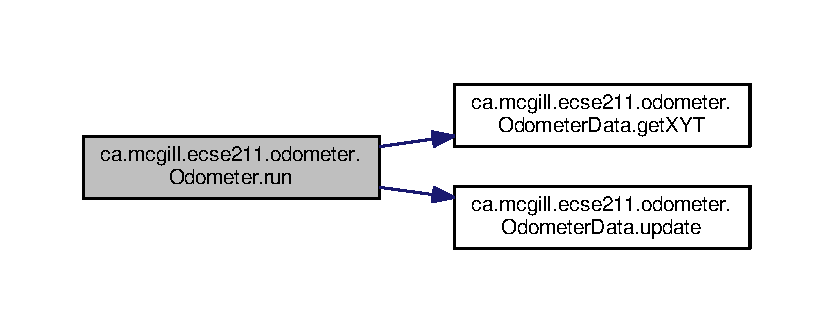
\includegraphics[width=350pt]{classca_1_1mcgill_1_1ecse211_1_1odometer_1_1_odometer_af0ff4c5121973a8310cf986e25fa0d87_cgraph}
\end{center}
\end{figure}


The documentation for this class was generated from the following file\+:\begin{DoxyCompactItemize}
\item 
/home/ccc/\+Final\+Project/src/ca/mcgill/ecse211/odometer/Odometer.\+java\end{DoxyCompactItemize}

\hypertarget{classca_1_1mcgill_1_1ecse211_1_1odometer_1_1_odometer_data}{}\section{ca.\+mcgill.\+ecse211.\+odometer.\+Odometer\+Data Class Reference}
\label{classca_1_1mcgill_1_1ecse211_1_1odometer_1_1_odometer_data}\index{ca.\+mcgill.\+ecse211.\+odometer.\+Odometer\+Data@{ca.\+mcgill.\+ecse211.\+odometer.\+Odometer\+Data}}


Inheritance diagram for ca.\+mcgill.\+ecse211.\+odometer.\+Odometer\+Data\+:\nopagebreak
\begin{figure}[H]
\begin{center}
\leavevmode
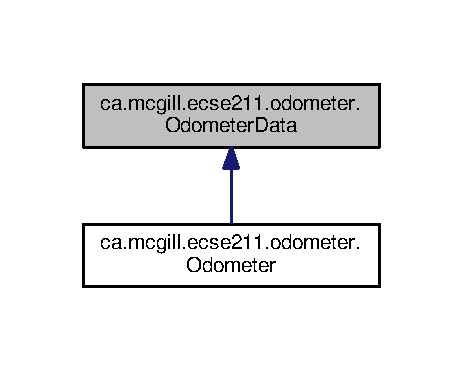
\includegraphics[width=222pt]{classca_1_1mcgill_1_1ecse211_1_1odometer_1_1_odometer_data__inherit__graph}
\end{center}
\end{figure}
\subsection*{Public Member Functions}
\begin{DoxyCompactItemize}
\item 
double \mbox{[}$\,$\mbox{]} \hyperlink{classca_1_1mcgill_1_1ecse211_1_1odometer_1_1_odometer_data_a8f40f0264c68f0cbed4fff1723ae7863}{get\+X\+YT} ()
\item 
void \hyperlink{classca_1_1mcgill_1_1ecse211_1_1odometer_1_1_odometer_data_aaa06f190d634299fcb1b97a1891dad85}{update} (double dx, double dy, double dtheta)
\item 
void \hyperlink{classca_1_1mcgill_1_1ecse211_1_1odometer_1_1_odometer_data_a2ebc18a13aea6276122d9ef4ee100bb9}{set\+X\+YT} (double x, double y, double theta)
\item 
void \hyperlink{classca_1_1mcgill_1_1ecse211_1_1odometer_1_1_odometer_data_a2911d7215e47f3064defe016b46bfeef}{setX} (double x)
\item 
void \hyperlink{classca_1_1mcgill_1_1ecse211_1_1odometer_1_1_odometer_data_a82986438cd462e66520bc62bb4bd2b75}{setY} (double y)
\item 
void \hyperlink{classca_1_1mcgill_1_1ecse211_1_1odometer_1_1_odometer_data_a419b8f07c2c5374411c8e62298e9a402}{set\+Theta} (double theta)
\end{DoxyCompactItemize}
\subsection*{Static Public Member Functions}
\begin{DoxyCompactItemize}
\item 
static synchronized \hyperlink{classca_1_1mcgill_1_1ecse211_1_1odometer_1_1_odometer_data}{Odometer\+Data} \hyperlink{classca_1_1mcgill_1_1ecse211_1_1odometer_1_1_odometer_data_afff2d760dd1f861b580f3eacef37f1cc}{get\+Odometer\+Data} ()  throws Odometer\+Exceptions 
\end{DoxyCompactItemize}
\subsection*{Protected Member Functions}
\begin{DoxyCompactItemize}
\item 
\hyperlink{classca_1_1mcgill_1_1ecse211_1_1odometer_1_1_odometer_data_a91412854b75c41bf3af7c8892ec0fe87}{Odometer\+Data} ()
\end{DoxyCompactItemize}


\subsection{Detailed Description}
This class stores and provides thread safe access to data required used by the \hyperlink{classca_1_1mcgill_1_1ecse211_1_1odometer_1_1_odometer}{Odometer} classes.

\begin{DoxyAuthor}{Author}
Caspar Cedro 

Percy Chen 

Patrick Erath 

Anssam Ghezala 

Susan Matuszewski 

Kamy Moussavi Kafi 
\end{DoxyAuthor}


Definition at line 17 of file Odometer\+Data.\+java.



\subsection{Constructor \& Destructor Documentation}
\mbox{\Hypertarget{classca_1_1mcgill_1_1ecse211_1_1odometer_1_1_odometer_data_a91412854b75c41bf3af7c8892ec0fe87}\label{classca_1_1mcgill_1_1ecse211_1_1odometer_1_1_odometer_data_a91412854b75c41bf3af7c8892ec0fe87}} 
\index{ca\+::mcgill\+::ecse211\+::odometer\+::\+Odometer\+Data@{ca\+::mcgill\+::ecse211\+::odometer\+::\+Odometer\+Data}!Odometer\+Data@{Odometer\+Data}}
\index{Odometer\+Data@{Odometer\+Data}!ca\+::mcgill\+::ecse211\+::odometer\+::\+Odometer\+Data@{ca\+::mcgill\+::ecse211\+::odometer\+::\+Odometer\+Data}}
\subsubsection{\texorpdfstring{Odometer\+Data()}{OdometerData()}}
{\footnotesize\ttfamily ca.\+mcgill.\+ecse211.\+odometer.\+Odometer\+Data.\+Odometer\+Data (\begin{DoxyParamCaption}{ }\end{DoxyParamCaption})\hspace{0.3cm}{\ttfamily [protected]}}

This is the class constructor for the \hyperlink{classca_1_1mcgill_1_1ecse211_1_1odometer_1_1_odometer_data}{Odometer\+Data} class. It cannot be instantiated externally. A factory is used instead such that only one instance of this class is ever created. 

Definition at line 47 of file Odometer\+Data.\+java.


\begin{DoxyCode}
47                            \{
48     this.x = 0;
49     this.y = 0;
50     this.theta = 0;
51   \}
\end{DoxyCode}
Here is the caller graph for this function\+:\nopagebreak
\begin{figure}[H]
\begin{center}
\leavevmode
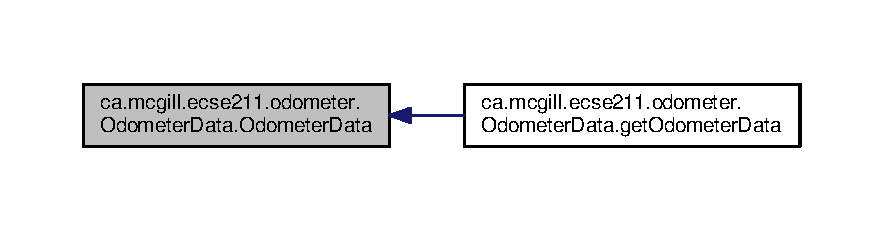
\includegraphics[width=350pt]{classca_1_1mcgill_1_1ecse211_1_1odometer_1_1_odometer_data_a91412854b75c41bf3af7c8892ec0fe87_icgraph}
\end{center}
\end{figure}


\subsection{Member Function Documentation}
\mbox{\Hypertarget{classca_1_1mcgill_1_1ecse211_1_1odometer_1_1_odometer_data_afff2d760dd1f861b580f3eacef37f1cc}\label{classca_1_1mcgill_1_1ecse211_1_1odometer_1_1_odometer_data_afff2d760dd1f861b580f3eacef37f1cc}} 
\index{ca\+::mcgill\+::ecse211\+::odometer\+::\+Odometer\+Data@{ca\+::mcgill\+::ecse211\+::odometer\+::\+Odometer\+Data}!get\+Odometer\+Data@{get\+Odometer\+Data}}
\index{get\+Odometer\+Data@{get\+Odometer\+Data}!ca\+::mcgill\+::ecse211\+::odometer\+::\+Odometer\+Data@{ca\+::mcgill\+::ecse211\+::odometer\+::\+Odometer\+Data}}
\subsubsection{\texorpdfstring{get\+Odometer\+Data()}{getOdometerData()}}
{\footnotesize\ttfamily static synchronized \hyperlink{classca_1_1mcgill_1_1ecse211_1_1odometer_1_1_odometer_data}{Odometer\+Data} ca.\+mcgill.\+ecse211.\+odometer.\+Odometer\+Data.\+get\+Odometer\+Data (\begin{DoxyParamCaption}{ }\end{DoxyParamCaption}) throws \hyperlink{classca_1_1mcgill_1_1ecse211_1_1odometer_1_1_odometer_exceptions}{Odometer\+Exceptions}\hspace{0.3cm}{\ttfamily [static]}}

This method returns an \hyperlink{classca_1_1mcgill_1_1ecse211_1_1odometer_1_1_odometer_data}{Odometer\+Data} instance and makes sure that only one instance is ever created.

\begin{DoxyReturn}{Returns}
An \hyperlink{classca_1_1mcgill_1_1ecse211_1_1odometer_1_1_odometer_data}{Odometer\+Data} object 
\end{DoxyReturn}

\begin{DoxyExceptions}{Exceptions}
{\em \hyperlink{classca_1_1mcgill_1_1ecse211_1_1odometer_1_1_odometer_exceptions}{Odometer\+Exceptions}} & \\
\hline
\end{DoxyExceptions}


Definition at line 60 of file Odometer\+Data.\+java.


\begin{DoxyCode}
60                                                                                       \{
61     \textcolor{keywordflow}{if} (odoData != null) \{ \textcolor{comment}{// Return existing object}
62       \textcolor{keywordflow}{return} odoData;
63     \} \textcolor{keywordflow}{else} \textcolor{keywordflow}{if} (numberOfIntances < MAX\_INSTANCES) \{
64       \textcolor{comment}{// create object and return it}
65       odoData = \textcolor{keyword}{new} \hyperlink{classca_1_1mcgill_1_1ecse211_1_1odometer_1_1_odometer_data_a91412854b75c41bf3af7c8892ec0fe87}{OdometerData}();
66       numberOfIntances += 1;
67       \textcolor{keywordflow}{return} odoData;
68     \} \textcolor{keywordflow}{else} \{
69       \textcolor{keywordflow}{throw} \textcolor{keyword}{new} OdometerExceptions(\textcolor{stringliteral}{"Only one intance of the Odometer can be created."});
70     \}
71   \}
\end{DoxyCode}
Here is the call graph for this function\+:\nopagebreak
\begin{figure}[H]
\begin{center}
\leavevmode
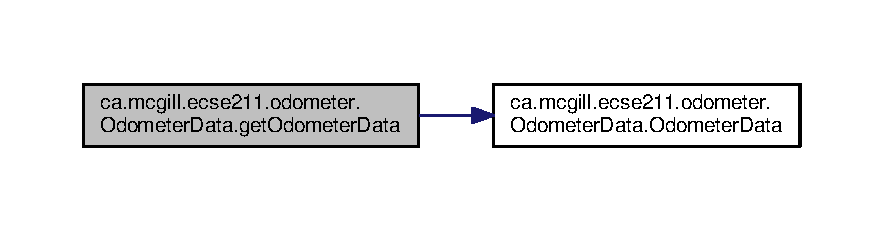
\includegraphics[width=350pt]{classca_1_1mcgill_1_1ecse211_1_1odometer_1_1_odometer_data_afff2d760dd1f861b580f3eacef37f1cc_cgraph}
\end{center}
\end{figure}
\mbox{\Hypertarget{classca_1_1mcgill_1_1ecse211_1_1odometer_1_1_odometer_data_a8f40f0264c68f0cbed4fff1723ae7863}\label{classca_1_1mcgill_1_1ecse211_1_1odometer_1_1_odometer_data_a8f40f0264c68f0cbed4fff1723ae7863}} 
\index{ca\+::mcgill\+::ecse211\+::odometer\+::\+Odometer\+Data@{ca\+::mcgill\+::ecse211\+::odometer\+::\+Odometer\+Data}!get\+X\+YT@{get\+X\+YT}}
\index{get\+X\+YT@{get\+X\+YT}!ca\+::mcgill\+::ecse211\+::odometer\+::\+Odometer\+Data@{ca\+::mcgill\+::ecse211\+::odometer\+::\+Odometer\+Data}}
\subsubsection{\texorpdfstring{get\+X\+Y\+T()}{getXYT()}}
{\footnotesize\ttfamily double \mbox{[}$\,$\mbox{]} ca.\+mcgill.\+ecse211.\+odometer.\+Odometer\+Data.\+get\+X\+YT (\begin{DoxyParamCaption}{ }\end{DoxyParamCaption})}

This method returns the \hyperlink{classca_1_1mcgill_1_1ecse211_1_1odometer_1_1_odometer}{Odometer} data. Writes the current position and orientation of the robot onto the odo\+Data array. odo\+Data\mbox{[}0\mbox{]} = x, odo\+Data\mbox{[}1\mbox{]} = y; odo\+Data\mbox{[}2\mbox{]} = theta;


\begin{DoxyParams}{Parameters}
{\em position} & the array to store the odometer data \\
\hline
\end{DoxyParams}
\begin{DoxyReturn}{Returns}
the odometer data. 
\end{DoxyReturn}


Definition at line 81 of file Odometer\+Data.\+java.


\begin{DoxyCode}
81                            \{
82     \textcolor{keywordtype}{double}[] position = \textcolor{keyword}{new} \textcolor{keywordtype}{double}[4];
83     lock.lock();
84     \textcolor{keywordflow}{try} \{
85       \textcolor{keywordflow}{while} (isReseting) \{ \textcolor{comment}{// If a reset operation is being executed, wait}
86         \textcolor{comment}{// until it is over.}
87         doneReseting.await(); \textcolor{comment}{// Using await() is lighter on the CPU}
88         \textcolor{comment}{// than simple busy wait.}
89       \}
90 
91       position[0] = x;
92       position[1] = y;
93       position[2] = theta;
94 
95     \} \textcolor{keywordflow}{catch} (InterruptedException e) \{
96       \textcolor{comment}{// Print exception to screen}
97       e.printStackTrace();
98     \} \textcolor{keywordflow}{finally} \{
99       lock.unlock();
100     \}
101 
102     \textcolor{keywordflow}{return} position;
103   \}
\end{DoxyCode}
Here is the caller graph for this function\+:\nopagebreak
\begin{figure}[H]
\begin{center}
\leavevmode
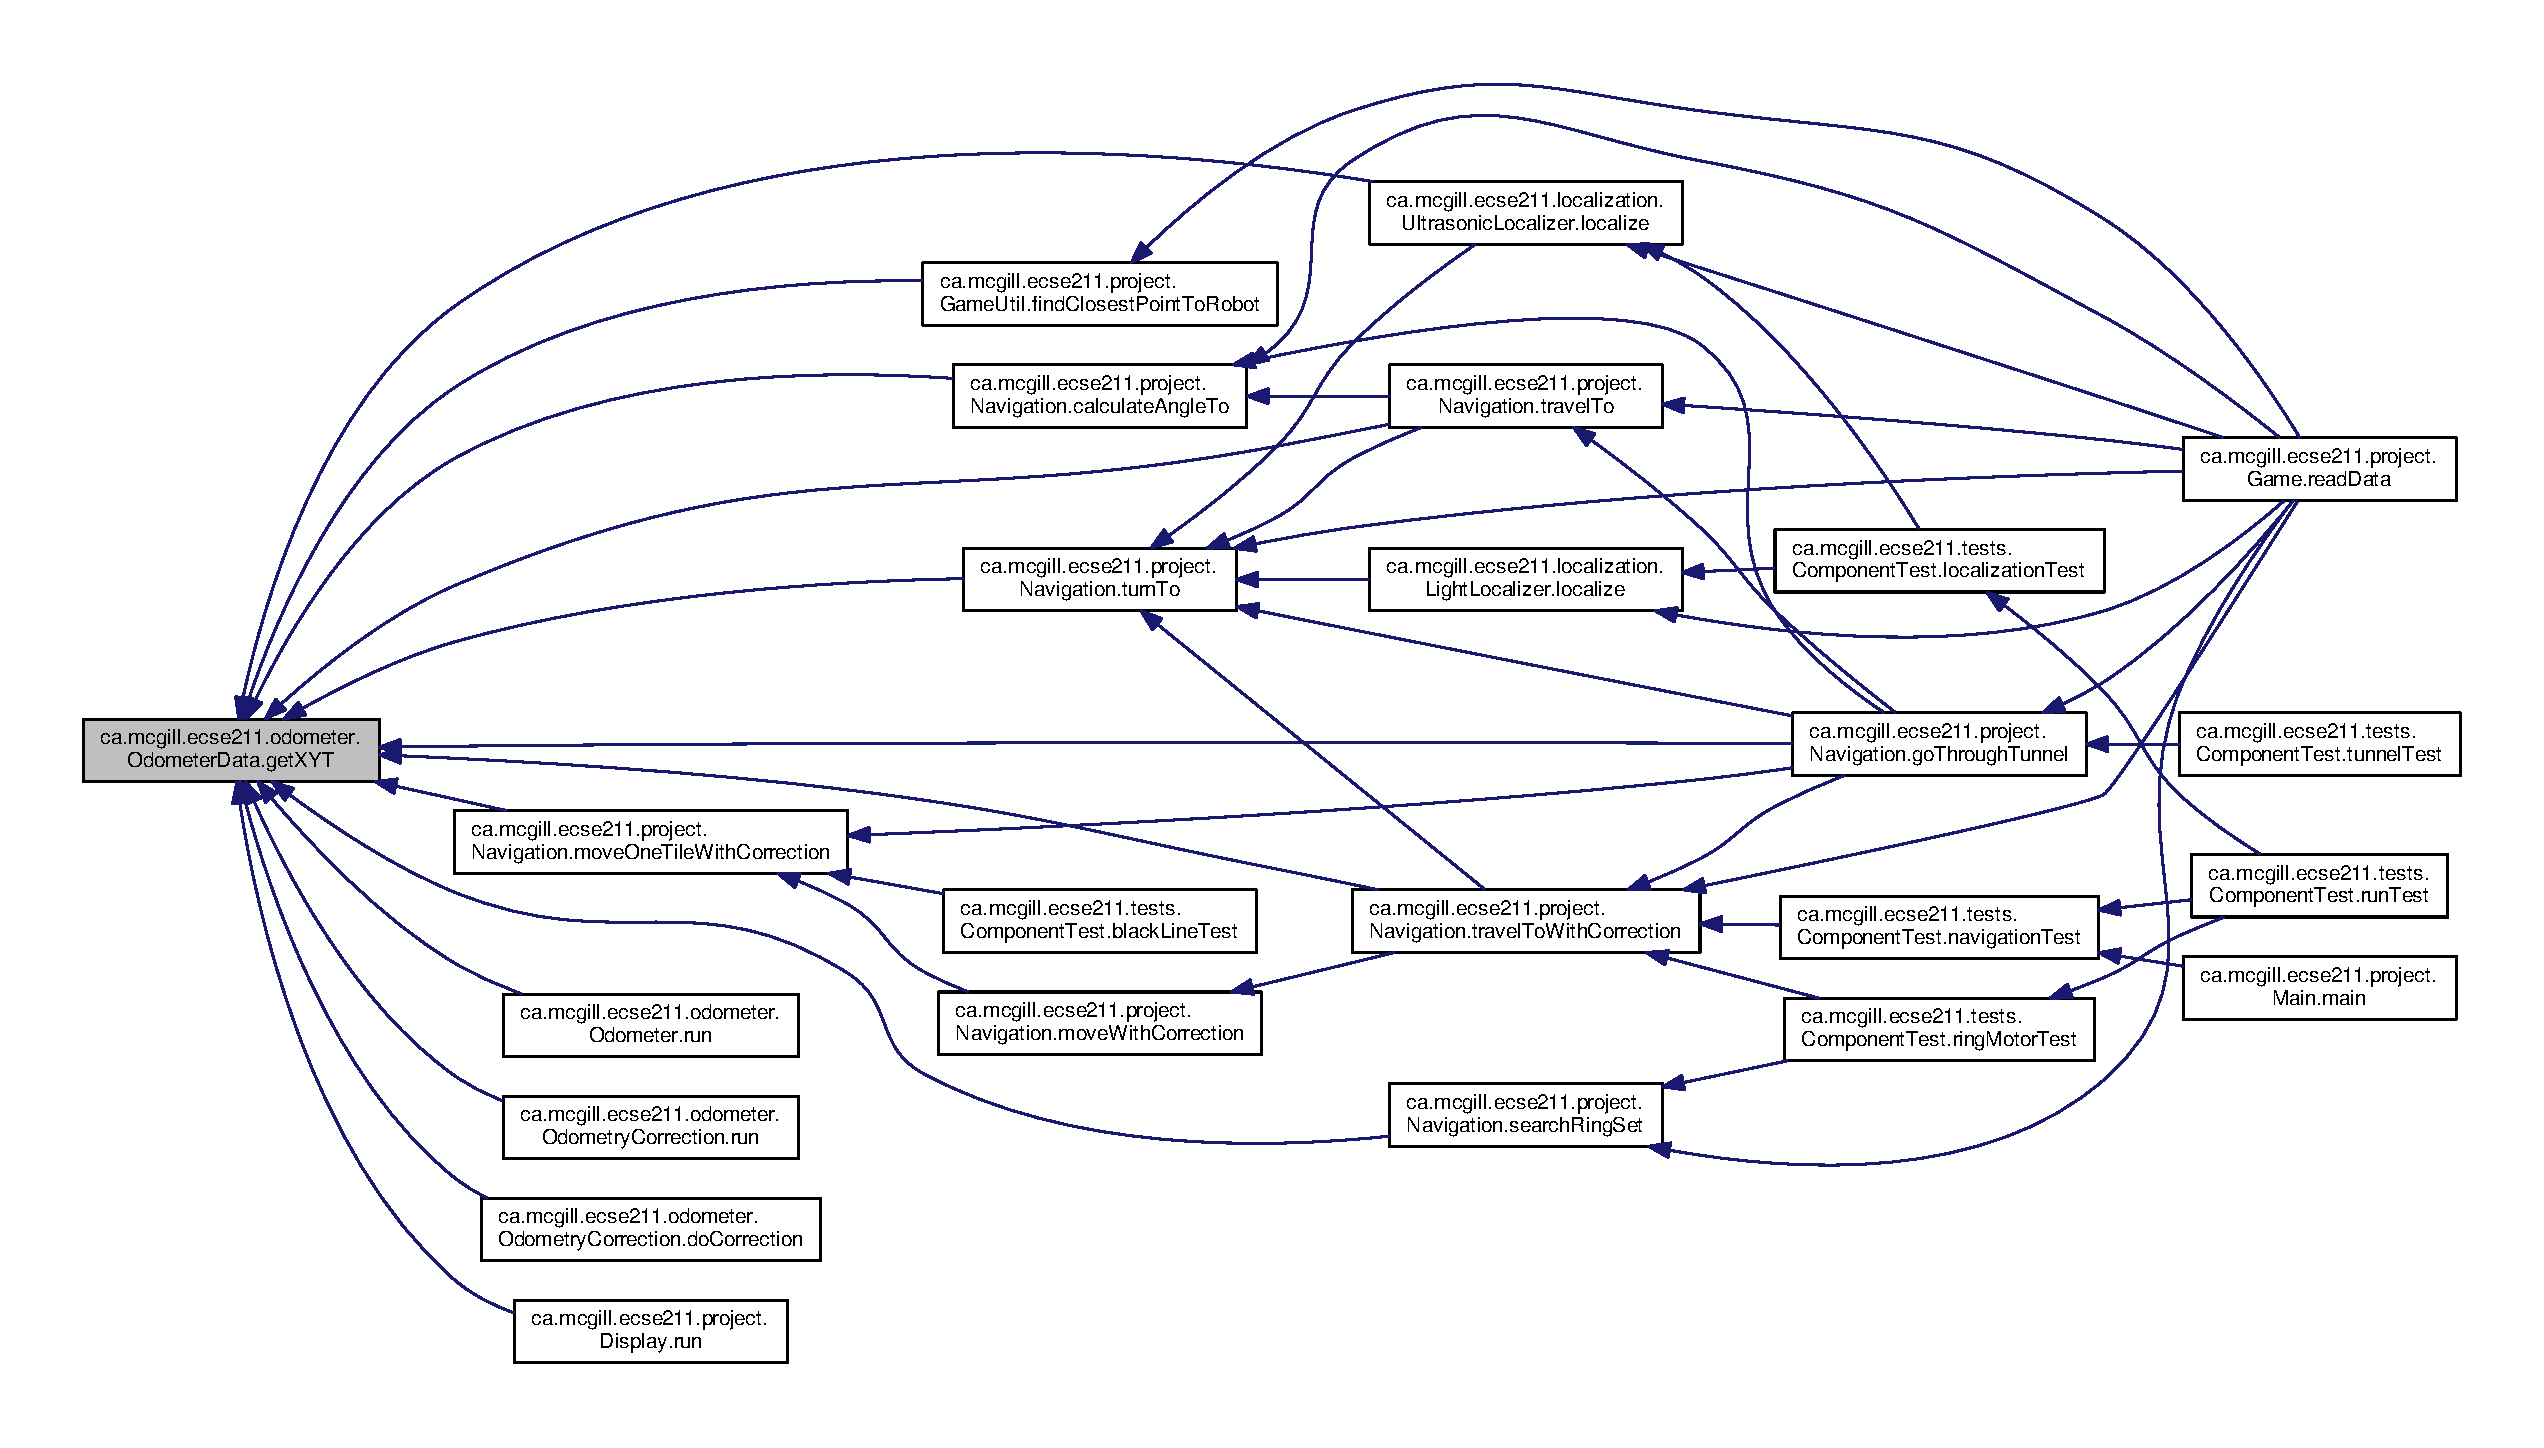
\includegraphics[width=350pt]{classca_1_1mcgill_1_1ecse211_1_1odometer_1_1_odometer_data_a8f40f0264c68f0cbed4fff1723ae7863_icgraph}
\end{center}
\end{figure}
\mbox{\Hypertarget{classca_1_1mcgill_1_1ecse211_1_1odometer_1_1_odometer_data_a419b8f07c2c5374411c8e62298e9a402}\label{classca_1_1mcgill_1_1ecse211_1_1odometer_1_1_odometer_data_a419b8f07c2c5374411c8e62298e9a402}} 
\index{ca\+::mcgill\+::ecse211\+::odometer\+::\+Odometer\+Data@{ca\+::mcgill\+::ecse211\+::odometer\+::\+Odometer\+Data}!set\+Theta@{set\+Theta}}
\index{set\+Theta@{set\+Theta}!ca\+::mcgill\+::ecse211\+::odometer\+::\+Odometer\+Data@{ca\+::mcgill\+::ecse211\+::odometer\+::\+Odometer\+Data}}
\subsubsection{\texorpdfstring{set\+Theta()}{setTheta()}}
{\footnotesize\ttfamily void ca.\+mcgill.\+ecse211.\+odometer.\+Odometer\+Data.\+set\+Theta (\begin{DoxyParamCaption}\item[{double}]{theta }\end{DoxyParamCaption})}

Overrides theta. Use for odometry correction.


\begin{DoxyParams}{Parameters}
{\em theta} & the value of theta \\
\hline
\end{DoxyParams}


Definition at line 194 of file Odometer\+Data.\+java.


\begin{DoxyCode}
194                                      \{
195     lock.lock();
196     isReseting = \textcolor{keyword}{true};
197     \textcolor{keywordflow}{try} \{
198       this.theta = theta;
199       isReseting = \textcolor{keyword}{false}; \textcolor{comment}{// Done reseting}
200       doneReseting.signalAll(); \textcolor{comment}{// Let the other threads know that you are}
201                                 \textcolor{comment}{// done reseting}
202     \} \textcolor{keywordflow}{finally} \{
203       lock.unlock();
204     \}
205   \}
\end{DoxyCode}
Here is the caller graph for this function\+:\nopagebreak
\begin{figure}[H]
\begin{center}
\leavevmode
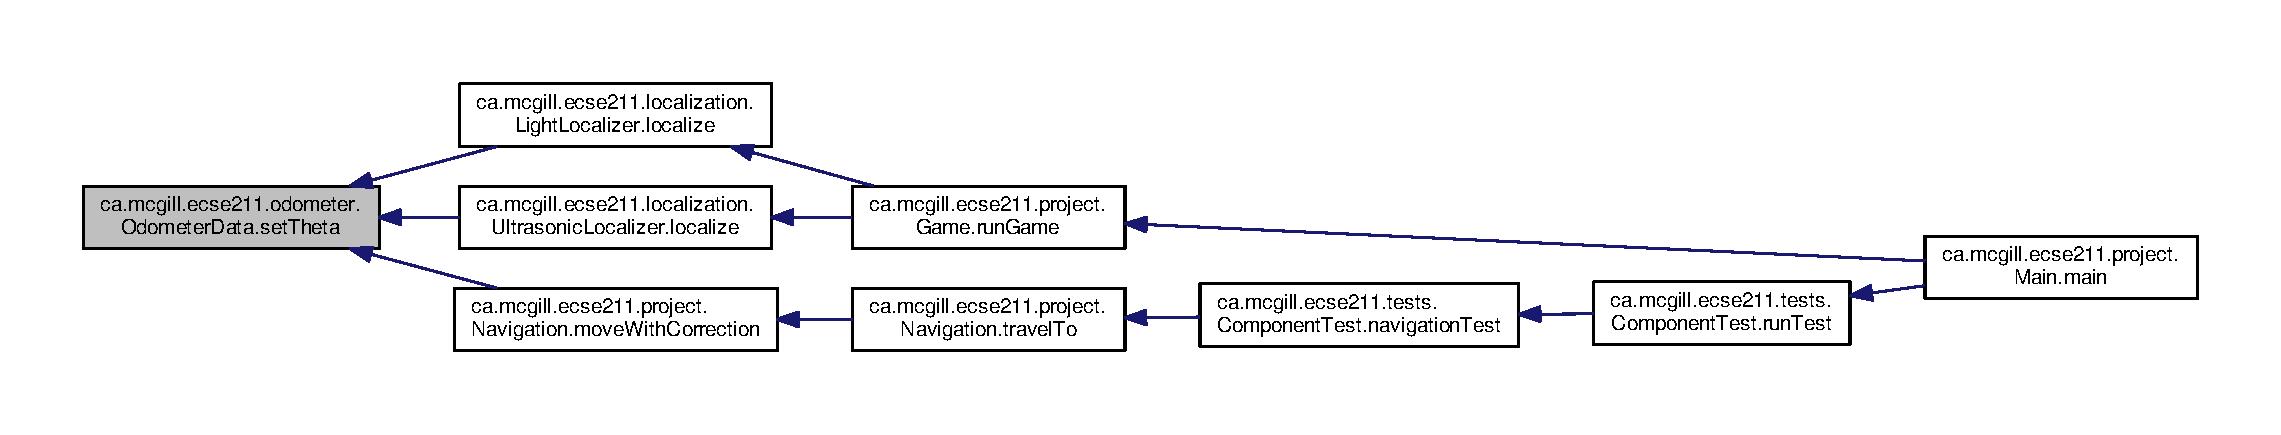
\includegraphics[width=350pt]{classca_1_1mcgill_1_1ecse211_1_1odometer_1_1_odometer_data_a419b8f07c2c5374411c8e62298e9a402_icgraph}
\end{center}
\end{figure}
\mbox{\Hypertarget{classca_1_1mcgill_1_1ecse211_1_1odometer_1_1_odometer_data_a2911d7215e47f3064defe016b46bfeef}\label{classca_1_1mcgill_1_1ecse211_1_1odometer_1_1_odometer_data_a2911d7215e47f3064defe016b46bfeef}} 
\index{ca\+::mcgill\+::ecse211\+::odometer\+::\+Odometer\+Data@{ca\+::mcgill\+::ecse211\+::odometer\+::\+Odometer\+Data}!setX@{setX}}
\index{setX@{setX}!ca\+::mcgill\+::ecse211\+::odometer\+::\+Odometer\+Data@{ca\+::mcgill\+::ecse211\+::odometer\+::\+Odometer\+Data}}
\subsubsection{\texorpdfstring{set\+X()}{setX()}}
{\footnotesize\ttfamily void ca.\+mcgill.\+ecse211.\+odometer.\+Odometer\+Data.\+setX (\begin{DoxyParamCaption}\item[{double}]{x }\end{DoxyParamCaption})}

Overrides x. Use for odometry correction.


\begin{DoxyParams}{Parameters}
{\em x} & the value of x \\
\hline
\end{DoxyParams}


Definition at line 158 of file Odometer\+Data.\+java.


\begin{DoxyCode}
158                              \{
159     lock.lock();
160     isReseting = \textcolor{keyword}{true};
161     \textcolor{keywordflow}{try} \{
162       this.x = x;
163       isReseting = \textcolor{keyword}{false}; \textcolor{comment}{// Done reseting}
164       doneReseting.signalAll(); \textcolor{comment}{// Let the other threads know that you are}
165                                 \textcolor{comment}{// done reseting}
166     \} \textcolor{keywordflow}{finally} \{
167       lock.unlock();
168     \}
169   \}
\end{DoxyCode}
Here is the caller graph for this function\+:\nopagebreak
\begin{figure}[H]
\begin{center}
\leavevmode
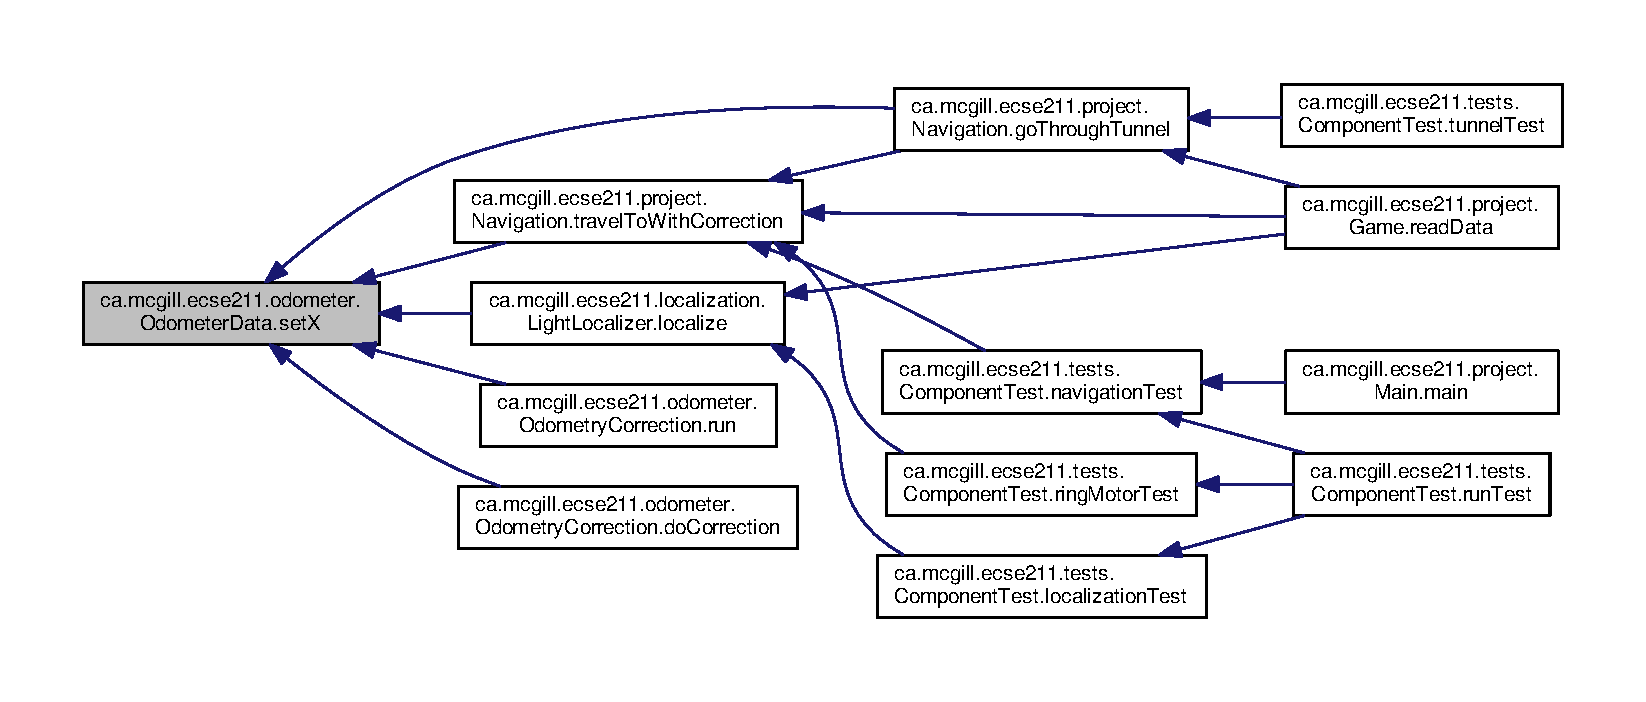
\includegraphics[width=350pt]{classca_1_1mcgill_1_1ecse211_1_1odometer_1_1_odometer_data_a2911d7215e47f3064defe016b46bfeef_icgraph}
\end{center}
\end{figure}
\mbox{\Hypertarget{classca_1_1mcgill_1_1ecse211_1_1odometer_1_1_odometer_data_a2ebc18a13aea6276122d9ef4ee100bb9}\label{classca_1_1mcgill_1_1ecse211_1_1odometer_1_1_odometer_data_a2ebc18a13aea6276122d9ef4ee100bb9}} 
\index{ca\+::mcgill\+::ecse211\+::odometer\+::\+Odometer\+Data@{ca\+::mcgill\+::ecse211\+::odometer\+::\+Odometer\+Data}!set\+X\+YT@{set\+X\+YT}}
\index{set\+X\+YT@{set\+X\+YT}!ca\+::mcgill\+::ecse211\+::odometer\+::\+Odometer\+Data@{ca\+::mcgill\+::ecse211\+::odometer\+::\+Odometer\+Data}}
\subsubsection{\texorpdfstring{set\+X\+Y\+T()}{setXYT()}}
{\footnotesize\ttfamily void ca.\+mcgill.\+ecse211.\+odometer.\+Odometer\+Data.\+set\+X\+YT (\begin{DoxyParamCaption}\item[{double}]{x,  }\item[{double}]{y,  }\item[{double}]{theta }\end{DoxyParamCaption})}

Overrides the values of x, y and theta. Use for odometry correction.


\begin{DoxyParams}{Parameters}
{\em x} & the value of x \\
\hline
{\em y} & the value of y \\
\hline
{\em theta} & the value of theta \\
\hline
\end{DoxyParams}


Definition at line 138 of file Odometer\+Data.\+java.


\begin{DoxyCode}
138                                                        \{
139     lock.lock();
140     isReseting = \textcolor{keyword}{true};
141     \textcolor{keywordflow}{try} \{
142       this.x = x;
143       this.y = y;
144       this.theta = theta;
145       isReseting = \textcolor{keyword}{false}; \textcolor{comment}{// Done reseting}
146       doneReseting.signalAll(); \textcolor{comment}{// Let the other threads know that you are}
147                                 \textcolor{comment}{// done reseting}
148     \} \textcolor{keywordflow}{finally} \{
149       lock.unlock();
150     \}
151   \}
\end{DoxyCode}
Here is the caller graph for this function\+:\nopagebreak
\begin{figure}[H]
\begin{center}
\leavevmode
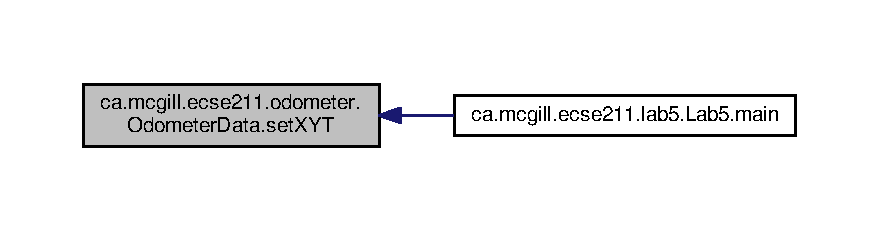
\includegraphics[width=350pt]{classca_1_1mcgill_1_1ecse211_1_1odometer_1_1_odometer_data_a2ebc18a13aea6276122d9ef4ee100bb9_icgraph}
\end{center}
\end{figure}
\mbox{\Hypertarget{classca_1_1mcgill_1_1ecse211_1_1odometer_1_1_odometer_data_a82986438cd462e66520bc62bb4bd2b75}\label{classca_1_1mcgill_1_1ecse211_1_1odometer_1_1_odometer_data_a82986438cd462e66520bc62bb4bd2b75}} 
\index{ca\+::mcgill\+::ecse211\+::odometer\+::\+Odometer\+Data@{ca\+::mcgill\+::ecse211\+::odometer\+::\+Odometer\+Data}!setY@{setY}}
\index{setY@{setY}!ca\+::mcgill\+::ecse211\+::odometer\+::\+Odometer\+Data@{ca\+::mcgill\+::ecse211\+::odometer\+::\+Odometer\+Data}}
\subsubsection{\texorpdfstring{set\+Y()}{setY()}}
{\footnotesize\ttfamily void ca.\+mcgill.\+ecse211.\+odometer.\+Odometer\+Data.\+setY (\begin{DoxyParamCaption}\item[{double}]{y }\end{DoxyParamCaption})}

Overrides y. Use for odometry correction.


\begin{DoxyParams}{Parameters}
{\em y} & the value of y \\
\hline
\end{DoxyParams}


Definition at line 176 of file Odometer\+Data.\+java.


\begin{DoxyCode}
176                              \{
177     lock.lock();
178     isReseting = \textcolor{keyword}{true};
179     \textcolor{keywordflow}{try} \{
180       this.y = y;
181       isReseting = \textcolor{keyword}{false}; \textcolor{comment}{// Done reseting}
182       doneReseting.signalAll(); \textcolor{comment}{// Let the other threads know that you are}
183                                 \textcolor{comment}{// done reseting}
184     \} \textcolor{keywordflow}{finally} \{
185       lock.unlock();
186     \}
187   \}
\end{DoxyCode}
Here is the caller graph for this function\+:\nopagebreak
\begin{figure}[H]
\begin{center}
\leavevmode
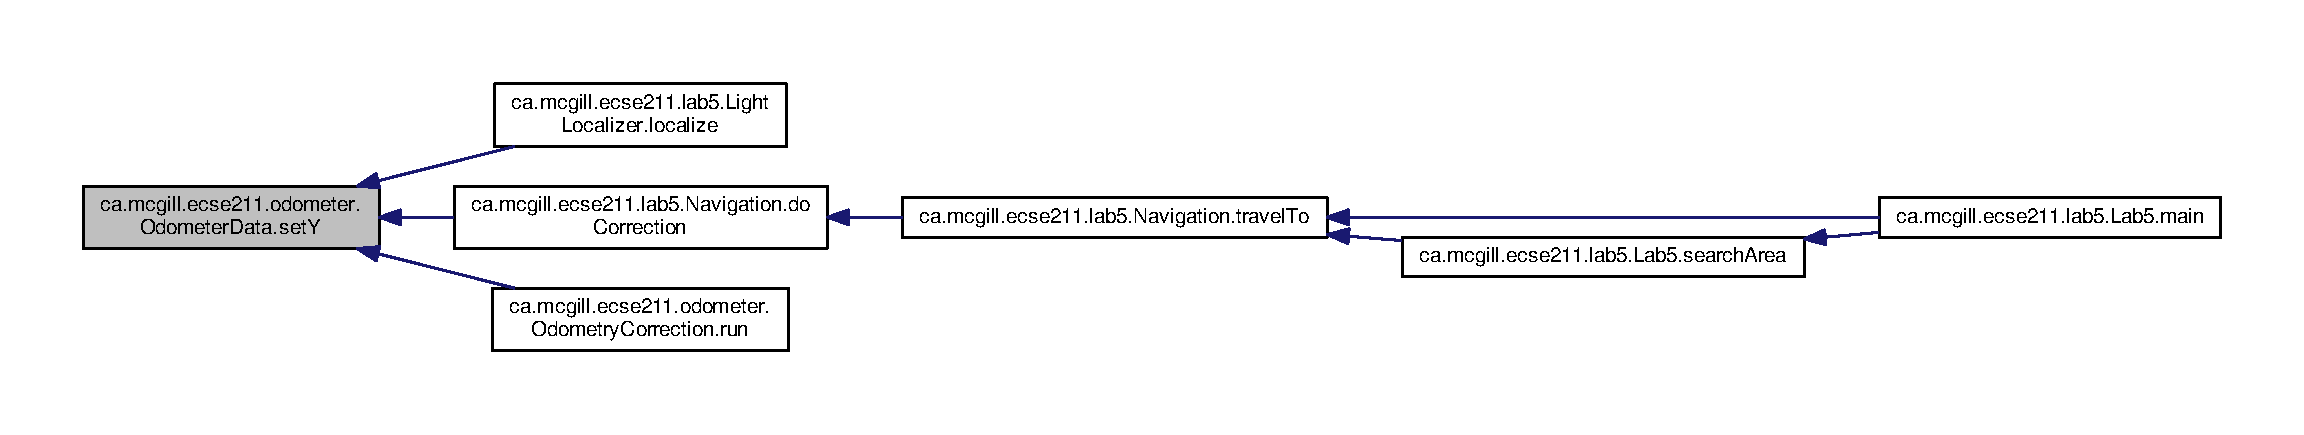
\includegraphics[width=350pt]{classca_1_1mcgill_1_1ecse211_1_1odometer_1_1_odometer_data_a82986438cd462e66520bc62bb4bd2b75_icgraph}
\end{center}
\end{figure}
\mbox{\Hypertarget{classca_1_1mcgill_1_1ecse211_1_1odometer_1_1_odometer_data_aaa06f190d634299fcb1b97a1891dad85}\label{classca_1_1mcgill_1_1ecse211_1_1odometer_1_1_odometer_data_aaa06f190d634299fcb1b97a1891dad85}} 
\index{ca\+::mcgill\+::ecse211\+::odometer\+::\+Odometer\+Data@{ca\+::mcgill\+::ecse211\+::odometer\+::\+Odometer\+Data}!update@{update}}
\index{update@{update}!ca\+::mcgill\+::ecse211\+::odometer\+::\+Odometer\+Data@{ca\+::mcgill\+::ecse211\+::odometer\+::\+Odometer\+Data}}
\subsubsection{\texorpdfstring{update()}{update()}}
{\footnotesize\ttfamily void ca.\+mcgill.\+ecse211.\+odometer.\+Odometer\+Data.\+update (\begin{DoxyParamCaption}\item[{double}]{dx,  }\item[{double}]{dy,  }\item[{double}]{dtheta }\end{DoxyParamCaption})}

Adds dx, dy and dtheta to the current values of x, y and theta, respectively. Useful for odometry.


\begin{DoxyParams}{Parameters}
{\em dx} & \\
\hline
{\em dy} & \\
\hline
{\em dtheta} & \\
\hline
\end{DoxyParams}


Definition at line 113 of file Odometer\+Data.\+java.


\begin{DoxyCode}
113                                                           \{
114     lock.lock();
115     isReseting = \textcolor{keyword}{true};
116     \textcolor{keywordflow}{try} \{
117       x += dx;
118       y += dy;
119       theta = (theta + (360 + dtheta) % 360) % 360; \textcolor{comment}{// keeps the updates}
120                                                     \textcolor{comment}{// within 360}
121                                                     \textcolor{comment}{// degrees}
122       isReseting = \textcolor{keyword}{false}; \textcolor{comment}{// Done reseting}
123       doneReseting.signalAll(); \textcolor{comment}{// Let the other threads know that you are}
124                                 \textcolor{comment}{// done reseting}
125     \} \textcolor{keywordflow}{finally} \{
126       lock.unlock();
127     \}
128 
129   \}
\end{DoxyCode}
Here is the caller graph for this function\+:\nopagebreak
\begin{figure}[H]
\begin{center}
\leavevmode
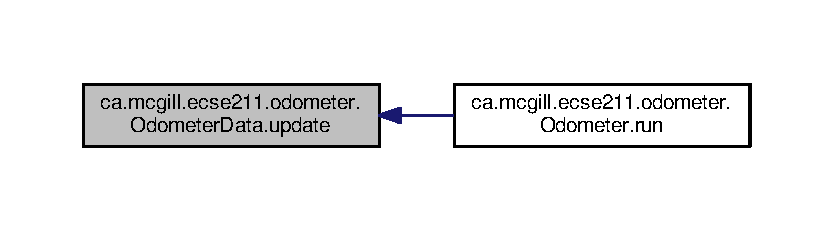
\includegraphics[width=350pt]{classca_1_1mcgill_1_1ecse211_1_1odometer_1_1_odometer_data_aaa06f190d634299fcb1b97a1891dad85_icgraph}
\end{center}
\end{figure}


The documentation for this class was generated from the following file\+:\begin{DoxyCompactItemize}
\item 
/home/ccc/\+Final\+Project/src/ca/mcgill/ecse211/odometer/\hyperlink{_odometer_data_8java}{Odometer\+Data.\+java}\end{DoxyCompactItemize}

\hypertarget{classca_1_1mcgill_1_1ecse211_1_1odometer_1_1_odometer_exceptions}{}\section{ca.\+mcgill.\+ecse211.\+odometer.\+Odometer\+Exceptions Class Reference}
\label{classca_1_1mcgill_1_1ecse211_1_1odometer_1_1_odometer_exceptions}\index{ca.\+mcgill.\+ecse211.\+odometer.\+Odometer\+Exceptions@{ca.\+mcgill.\+ecse211.\+odometer.\+Odometer\+Exceptions}}


Inheritance diagram for ca.\+mcgill.\+ecse211.\+odometer.\+Odometer\+Exceptions\+:
\nopagebreak
\begin{figure}[H]
\begin{center}
\leavevmode
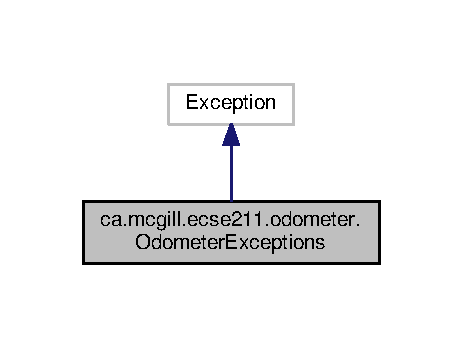
\includegraphics[width=222pt]{classca_1_1mcgill_1_1ecse211_1_1odometer_1_1_odometer_exceptions__inherit__graph}
\end{center}
\end{figure}


Collaboration diagram for ca.\+mcgill.\+ecse211.\+odometer.\+Odometer\+Exceptions\+:
\nopagebreak
\begin{figure}[H]
\begin{center}
\leavevmode
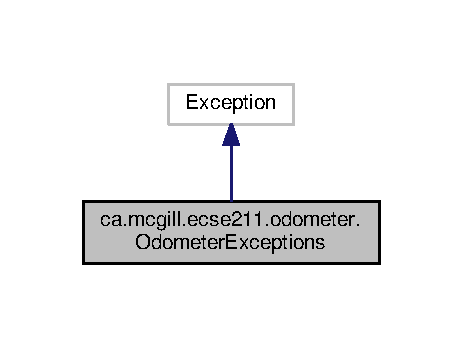
\includegraphics[width=222pt]{classca_1_1mcgill_1_1ecse211_1_1odometer_1_1_odometer_exceptions__coll__graph}
\end{center}
\end{figure}
\subsection*{Public Member Functions}
\begin{DoxyCompactItemize}
\item 
\hyperlink{classca_1_1mcgill_1_1ecse211_1_1odometer_1_1_odometer_exceptions_a25aa31baebe4906716a920929f0284d2}{Odometer\+Exceptions} (String Error)
\end{DoxyCompactItemize}


\subsection{Detailed Description}
This class is used to handle errors regarding the singleton pattern used for the odometer and odometer\+Data

\begin{DoxyAuthor}{Author}
Caspar Cedro \& Patrick Erath 
\end{DoxyAuthor}


Definition at line 10 of file Odometer\+Exceptions.\+java.



\subsection{Constructor \& Destructor Documentation}
\mbox{\Hypertarget{classca_1_1mcgill_1_1ecse211_1_1odometer_1_1_odometer_exceptions_a25aa31baebe4906716a920929f0284d2}\label{classca_1_1mcgill_1_1ecse211_1_1odometer_1_1_odometer_exceptions_a25aa31baebe4906716a920929f0284d2}} 
\index{ca\+::mcgill\+::ecse211\+::odometer\+::\+Odometer\+Exceptions@{ca\+::mcgill\+::ecse211\+::odometer\+::\+Odometer\+Exceptions}!Odometer\+Exceptions@{Odometer\+Exceptions}}
\index{Odometer\+Exceptions@{Odometer\+Exceptions}!ca\+::mcgill\+::ecse211\+::odometer\+::\+Odometer\+Exceptions@{ca\+::mcgill\+::ecse211\+::odometer\+::\+Odometer\+Exceptions}}
\subsubsection{\texorpdfstring{Odometer\+Exceptions()}{OdometerExceptions()}}
{\footnotesize\ttfamily ca.\+mcgill.\+ecse211.\+odometer.\+Odometer\+Exceptions.\+Odometer\+Exceptions (\begin{DoxyParamCaption}\item[{String}]{Error }\end{DoxyParamCaption})}

This is an \hyperlink{classca_1_1mcgill_1_1ecse211_1_1odometer_1_1_odometer_exceptions}{Odometer\+Exceptions} class constructor that accepts a descriptive error message.


\begin{DoxyParams}{Parameters}
{\em Error} & a String that contains an error message \\
\hline
\end{DoxyParams}


Definition at line 16 of file Odometer\+Exceptions.\+java.



The documentation for this class was generated from the following file\+:\begin{DoxyCompactItemize}
\item 
/home/ccc/\+Eclipse-\/\+Workspace-\/\+Oxygen/\+Lab5-\/\+Search\+And\+Localize/src/ca/mcgill/ecse211/odometer/Odometer\+Exceptions.\+java\end{DoxyCompactItemize}

\hypertarget{classca_1_1mcgill_1_1ecse211_1_1odometer_1_1_odometry_correction}{}\section{ca.\+mcgill.\+ecse211.\+odometer.\+Odometry\+Correction Class Reference}
\label{classca_1_1mcgill_1_1ecse211_1_1odometer_1_1_odometry_correction}\index{ca.\+mcgill.\+ecse211.\+odometer.\+Odometry\+Correction@{ca.\+mcgill.\+ecse211.\+odometer.\+Odometry\+Correction}}


Inheritance diagram for ca.\+mcgill.\+ecse211.\+odometer.\+Odometry\+Correction\+:\nopagebreak
\begin{figure}[H]
\begin{center}
\leavevmode
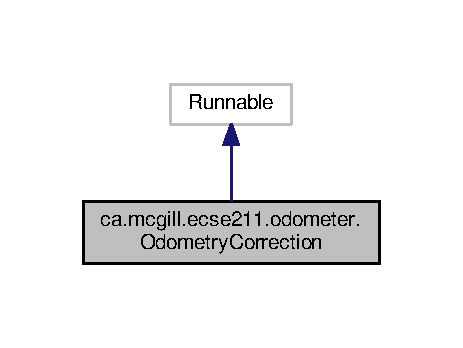
\includegraphics[width=222pt]{classca_1_1mcgill_1_1ecse211_1_1odometer_1_1_odometry_correction__inherit__graph}
\end{center}
\end{figure}


Collaboration diagram for ca.\+mcgill.\+ecse211.\+odometer.\+Odometry\+Correction\+:\nopagebreak
\begin{figure}[H]
\begin{center}
\leavevmode
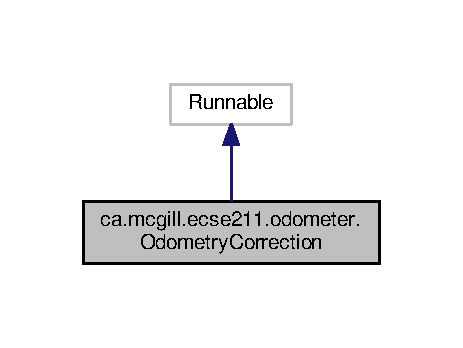
\includegraphics[width=222pt]{classca_1_1mcgill_1_1ecse211_1_1odometer_1_1_odometry_correction__coll__graph}
\end{center}
\end{figure}
\subsection*{Public Member Functions}
\begin{DoxyCompactItemize}
\item 
\hyperlink{classca_1_1mcgill_1_1ecse211_1_1odometer_1_1_odometry_correction_ad80b45e0bc4bf935494e075edcec739c}{Odometry\+Correction} ()  throws Odometer\+Exceptions 
\item 
void \hyperlink{classca_1_1mcgill_1_1ecse211_1_1odometer_1_1_odometry_correction_aad66a7030ac00f3a9cbe7bc33c25acbf}{run} ()
\item 
void \hyperlink{classca_1_1mcgill_1_1ecse211_1_1odometer_1_1_odometry_correction_a21a351682dc75060d6a5f15ad4775068}{do\+Correction} (double angle)
\end{DoxyCompactItemize}


\subsection{Detailed Description}
This class implements correction for the odometry on our robot using a light sensor.

\begin{DoxyAuthor}{Author}
Caspar Cedro 

Percy Chen 

Patrick Erath 

Anssam Ghezala 

Susan Matuszewski 

Kamy Moussavi Kafi 
\end{DoxyAuthor}


Definition at line 20 of file Odometry\+Correction.\+java.



\subsection{Constructor \& Destructor Documentation}
\mbox{\Hypertarget{classca_1_1mcgill_1_1ecse211_1_1odometer_1_1_odometry_correction_ad80b45e0bc4bf935494e075edcec739c}\label{classca_1_1mcgill_1_1ecse211_1_1odometer_1_1_odometry_correction_ad80b45e0bc4bf935494e075edcec739c}} 
\index{ca\+::mcgill\+::ecse211\+::odometer\+::\+Odometry\+Correction@{ca\+::mcgill\+::ecse211\+::odometer\+::\+Odometry\+Correction}!Odometry\+Correction@{Odometry\+Correction}}
\index{Odometry\+Correction@{Odometry\+Correction}!ca\+::mcgill\+::ecse211\+::odometer\+::\+Odometry\+Correction@{ca\+::mcgill\+::ecse211\+::odometer\+::\+Odometry\+Correction}}
\subsubsection{\texorpdfstring{Odometry\+Correction()}{OdometryCorrection()}}
{\footnotesize\ttfamily ca.\+mcgill.\+ecse211.\+odometer.\+Odometry\+Correction.\+Odometry\+Correction (\begin{DoxyParamCaption}{ }\end{DoxyParamCaption}) throws \hyperlink{classca_1_1mcgill_1_1ecse211_1_1odometer_1_1_odometer_exceptions}{Odometer\+Exceptions}}

This is the class constructor for the \hyperlink{classca_1_1mcgill_1_1ecse211_1_1odometer_1_1_odometry_correction}{Odometry\+Correction} class.


\begin{DoxyExceptions}{Exceptions}
{\em \hyperlink{classca_1_1mcgill_1_1ecse211_1_1odometer_1_1_odometer_exceptions}{Odometer\+Exceptions}} & \\
\hline
\end{DoxyExceptions}


Definition at line 35 of file Odometry\+Correction.\+java.


\begin{DoxyCode}
35                                                         \{
36     \textcolor{comment}{// Utilize the singleton Odometer object instance for thread safety.}
37     this.odometer = Odometer.\hyperlink{classca_1_1mcgill_1_1ecse211_1_1odometer_1_1_odometer_a99171f11e34dea918fa9dd069d721439}{getOdometer}();
38   \}
\end{DoxyCode}
Here is the call graph for this function\+:\nopagebreak
\begin{figure}[H]
\begin{center}
\leavevmode
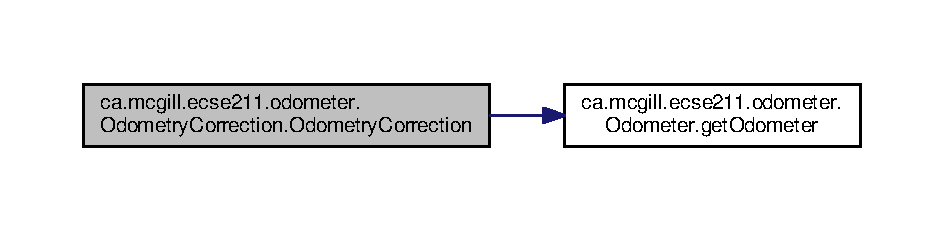
\includegraphics[width=350pt]{classca_1_1mcgill_1_1ecse211_1_1odometer_1_1_odometry_correction_ad80b45e0bc4bf935494e075edcec739c_cgraph}
\end{center}
\end{figure}


\subsection{Member Function Documentation}
\mbox{\Hypertarget{classca_1_1mcgill_1_1ecse211_1_1odometer_1_1_odometry_correction_a21a351682dc75060d6a5f15ad4775068}\label{classca_1_1mcgill_1_1ecse211_1_1odometer_1_1_odometry_correction_a21a351682dc75060d6a5f15ad4775068}} 
\index{ca\+::mcgill\+::ecse211\+::odometer\+::\+Odometry\+Correction@{ca\+::mcgill\+::ecse211\+::odometer\+::\+Odometry\+Correction}!do\+Correction@{do\+Correction}}
\index{do\+Correction@{do\+Correction}!ca\+::mcgill\+::ecse211\+::odometer\+::\+Odometry\+Correction@{ca\+::mcgill\+::ecse211\+::odometer\+::\+Odometry\+Correction}}
\subsubsection{\texorpdfstring{do\+Correction()}{doCorrection()}}
{\footnotesize\ttfamily void ca.\+mcgill.\+ecse211.\+odometer.\+Odometry\+Correction.\+do\+Correction (\begin{DoxyParamCaption}\item[{double}]{angle }\end{DoxyParamCaption})}

This method corrects our robot\textquotesingle{}s \hyperlink{classca_1_1mcgill_1_1ecse211_1_1odometer_1_1_odometer}{Odometer} readings


\begin{DoxyParams}{Parameters}
{\em angle} & The current angle that the robot is facing \\
\hline
\end{DoxyParams}


Definition at line 95 of file Odometry\+Correction.\+java.


\begin{DoxyCode}
95                                          \{
96     \textcolor{keywordtype}{double}[] position = odometer.\hyperlink{classca_1_1mcgill_1_1ecse211_1_1odometer_1_1_odometer_data_a8f40f0264c68f0cbed4fff1723ae7863}{getXYT}();
97     \textcolor{comment}{// Check that our robot's angle is within certain bounds and correct odometer if required.}
98     \textcolor{keywordflow}{if} (angle < 5 || angle > 355) \{
99       \textcolor{keywordtype}{int} sensorCoor = (int) Math.round(position[1] - SENSOR\_DIS / Game.TILE);
100       odometer.\hyperlink{classca_1_1mcgill_1_1ecse211_1_1odometer_1_1_odometer_data_a82986438cd462e66520bc62bb4bd2b75}{setY}(sensorCoor + SENSOR\_DIS / Game.TILE);
101     \} \textcolor{keywordflow}{else} \textcolor{keywordflow}{if} (angle < 185 && angle > 175) \{
102       \textcolor{keywordtype}{int} sensorCoor = (int) Math.round(position[1] + SENSOR\_DIS / Game.TILE);
103       odometer.\hyperlink{classca_1_1mcgill_1_1ecse211_1_1odometer_1_1_odometer_data_a82986438cd462e66520bc62bb4bd2b75}{setY}(sensorCoor - SENSOR\_DIS / Game.TILE);
104     \} \textcolor{keywordflow}{else} \textcolor{keywordflow}{if} (angle < 95 && angle > 85) \{
105       \textcolor{keywordtype}{int} sensorCoor = (int) Math.round(position[0] - SENSOR\_DIS / Game.TILE);
106       odometer.\hyperlink{classca_1_1mcgill_1_1ecse211_1_1odometer_1_1_odometer_data_a2911d7215e47f3064defe016b46bfeef}{setX}(sensorCoor + SENSOR\_DIS / Game.TILE);
107     \}
108   \}
\end{DoxyCode}
Here is the call graph for this function\+:\nopagebreak
\begin{figure}[H]
\begin{center}
\leavevmode
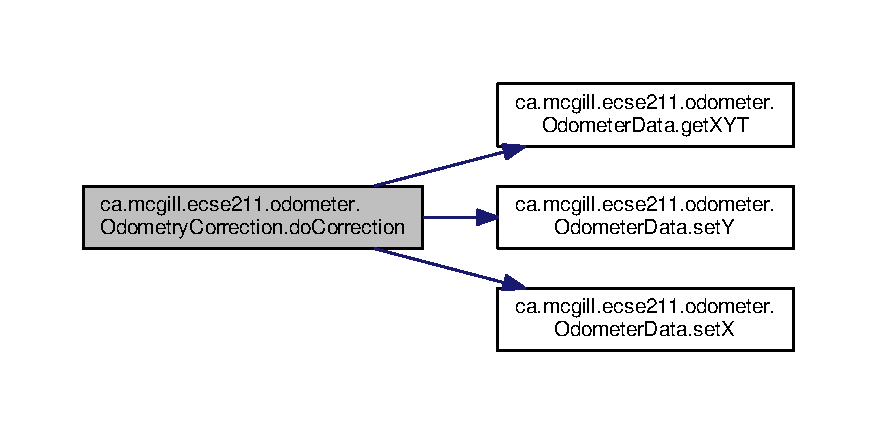
\includegraphics[width=350pt]{classca_1_1mcgill_1_1ecse211_1_1odometer_1_1_odometry_correction_a21a351682dc75060d6a5f15ad4775068_cgraph}
\end{center}
\end{figure}
\mbox{\Hypertarget{classca_1_1mcgill_1_1ecse211_1_1odometer_1_1_odometry_correction_aad66a7030ac00f3a9cbe7bc33c25acbf}\label{classca_1_1mcgill_1_1ecse211_1_1odometer_1_1_odometry_correction_aad66a7030ac00f3a9cbe7bc33c25acbf}} 
\index{ca\+::mcgill\+::ecse211\+::odometer\+::\+Odometry\+Correction@{ca\+::mcgill\+::ecse211\+::odometer\+::\+Odometry\+Correction}!run@{run}}
\index{run@{run}!ca\+::mcgill\+::ecse211\+::odometer\+::\+Odometry\+Correction@{ca\+::mcgill\+::ecse211\+::odometer\+::\+Odometry\+Correction}}
\subsubsection{\texorpdfstring{run()}{run()}}
{\footnotesize\ttfamily void ca.\+mcgill.\+ecse211.\+odometer.\+Odometry\+Correction.\+run (\begin{DoxyParamCaption}{ }\end{DoxyParamCaption})}

This method is called when this \hyperlink{classca_1_1mcgill_1_1ecse211_1_1odometer_1_1_odometry_correction}{Odometry\+Correction} object instance is started as a thread. Functionality wise it will correct the rotation and position of the robot once a black line is detected.


\begin{DoxyExceptions}{Exceptions}
{\em \hyperlink{classca_1_1mcgill_1_1ecse211_1_1odometer_1_1_odometer_exceptions}{Odometer\+Exceptions}} & \\
\hline
\end{DoxyExceptions}


Definition at line 47 of file Odometry\+Correction.\+java.


\begin{DoxyCode}
47                     \{
48     \textcolor{keywordtype}{long} correctionStart, correctionEnd;
49     \textcolor{keywordtype}{boolean} onTopOfLine = \textcolor{keyword}{false};
50 
51     \textcolor{keywordflow}{while} (\textcolor{keyword}{true}) \{
52       correctionStart = System.currentTimeMillis();
53 
54       \textcolor{comment}{// Fetch the sample at offset 0}
55       myColorSample.fetchSample(sampleColor, 0);
56 
57       \textcolor{comment}{// Check if our light sensor has read a black line and is not already on top of one}
58       \textcolor{keywordflow}{if} (sampleColor[0] < LINE\_COLOR\_THRESHOLD && !onTopOfLine) \{
59 
60         \textcolor{comment}{// New black line detected}
61         Sound.beep();
62         onTopOfLine = \textcolor{keyword}{true};
63 
64         \textcolor{keywordtype}{double} x = odometer.\hyperlink{classca_1_1mcgill_1_1ecse211_1_1odometer_1_1_odometer_data_a8f40f0264c68f0cbed4fff1723ae7863}{getXYT}()[0];
65         \textcolor{keywordtype}{double} y = odometer.\hyperlink{classca_1_1mcgill_1_1ecse211_1_1odometer_1_1_odometer_data_a8f40f0264c68f0cbed4fff1723ae7863}{getXYT}()[1];
66 
67         \textcolor{keywordflow}{if} (Math.abs(x % TILE\_WIDTH) < Math.abs(y % TILE\_WIDTH)) \{
68           odometer.\hyperlink{classca_1_1mcgill_1_1ecse211_1_1odometer_1_1_odometer_data_a2911d7215e47f3064defe016b46bfeef}{setX}(Math.round(x / TILE\_WIDTH) * TILE\_WIDTH);
69         \} \textcolor{keywordflow}{else} \{
70           odometer.\hyperlink{classca_1_1mcgill_1_1ecse211_1_1odometer_1_1_odometer_data_a82986438cd462e66520bc62bb4bd2b75}{setY}(Math.round(y / TILE\_WIDTH) * TILE\_WIDTH);
71         \}
72 
73       \} \textcolor{keywordflow}{else} \textcolor{keywordflow}{if} (sampleColor[0] > LINE\_COLOR\_THRESHOLD) \{
74         \textcolor{comment}{// No longer on top of line, reset to false}
75         onTopOfLine = \textcolor{keyword}{false};
76       \}
77 
78       \textcolor{comment}{// this ensure the odometry correction occurs only once every period}
79       correctionEnd = System.currentTimeMillis();
80       \textcolor{keywordflow}{if} (correctionEnd - correctionStart < CORRECTION\_PERIOD) \{
81         \textcolor{keywordflow}{try} \{
82           Thread.sleep(CORRECTION\_PERIOD - (correctionEnd - correctionStart));
83         \} \textcolor{keywordflow}{catch} (InterruptedException e) \{
84           \textcolor{comment}{// there is nothing to be done here}
85         \}
86       \}
87     \}
88   \}
\end{DoxyCode}
Here is the call graph for this function\+:\nopagebreak
\begin{figure}[H]
\begin{center}
\leavevmode
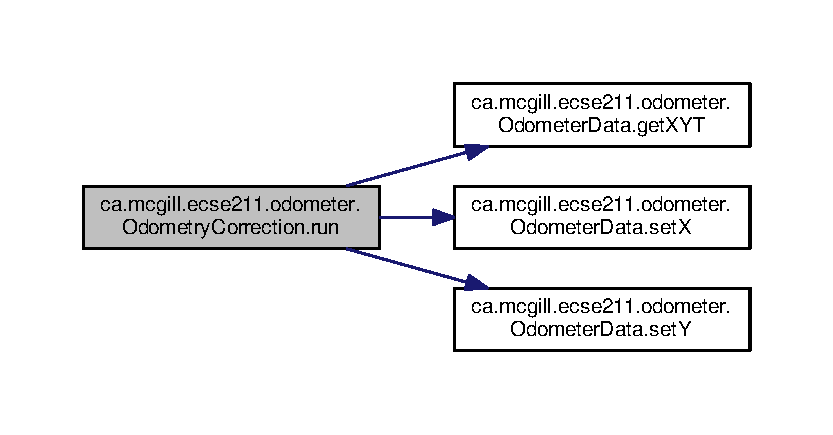
\includegraphics[width=350pt]{classca_1_1mcgill_1_1ecse211_1_1odometer_1_1_odometry_correction_aad66a7030ac00f3a9cbe7bc33c25acbf_cgraph}
\end{center}
\end{figure}


The documentation for this class was generated from the following file\+:\begin{DoxyCompactItemize}
\item 
/home/ccc/\+Final\+Project/src/ca/mcgill/ecse211/odometer/\hyperlink{_odometry_correction_8java}{Odometry\+Correction.\+java}\end{DoxyCompactItemize}

\hypertarget{classca_1_1mcgill_1_1ecse211_1_1sensors_1_1_r_g_b_poller}{}\section{ca.\+mcgill.\+ecse211.\+sensors.\+R\+G\+B\+Poller Class Reference}
\label{classca_1_1mcgill_1_1ecse211_1_1sensors_1_1_r_g_b_poller}\index{ca.\+mcgill.\+ecse211.\+sensors.\+R\+G\+B\+Poller@{ca.\+mcgill.\+ecse211.\+sensors.\+R\+G\+B\+Poller}}


Inheritance diagram for ca.\+mcgill.\+ecse211.\+sensors.\+R\+G\+B\+Poller\+:\nopagebreak
\begin{figure}[H]
\begin{center}
\leavevmode
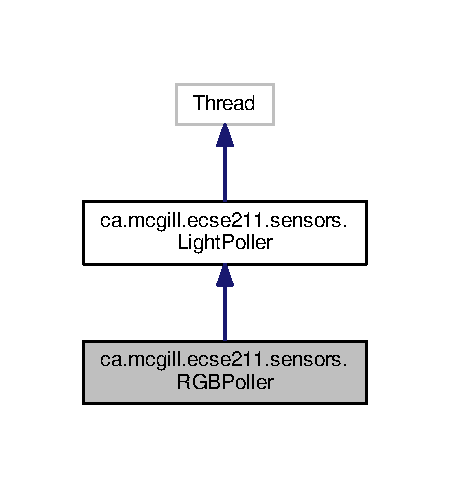
\includegraphics[width=216pt]{classca_1_1mcgill_1_1ecse211_1_1sensors_1_1_r_g_b_poller__inherit__graph}
\end{center}
\end{figure}


Collaboration diagram for ca.\+mcgill.\+ecse211.\+sensors.\+R\+G\+B\+Poller\+:\nopagebreak
\begin{figure}[H]
\begin{center}
\leavevmode
\includegraphics[width=350pt]{classca_1_1mcgill_1_1ecse211_1_1sensors_1_1_r_g_b_poller__coll__graph}
\end{center}
\end{figure}
\subsection*{Public Member Functions}
\begin{DoxyCompactItemize}
\item 
\mbox{\Hypertarget{classca_1_1mcgill_1_1ecse211_1_1sensors_1_1_r_g_b_poller_aa0e804f9185cb172aa1f63c62d13d168}\label{classca_1_1mcgill_1_1ecse211_1_1sensors_1_1_r_g_b_poller_aa0e804f9185cb172aa1f63c62d13d168}} 
{\bfseries R\+G\+B\+Poller} (Sample\+Provider us, float\mbox{[}$\,$\mbox{]} us\+Data, \hyperlink{classca_1_1mcgill_1_1ecse211_1_1sensors_1_1_sensor_data}{Sensor\+Data} cont)  throws Odometer\+Exceptions 
\end{DoxyCompactItemize}
\subsection*{Protected Member Functions}
\begin{DoxyCompactItemize}
\item 
\mbox{\Hypertarget{classca_1_1mcgill_1_1ecse211_1_1sensors_1_1_r_g_b_poller_aa24f4b9ce7425a82fbee017619a49234}\label{classca_1_1mcgill_1_1ecse211_1_1sensors_1_1_r_g_b_poller_aa24f4b9ce7425a82fbee017619a49234}} 
void {\bfseries process\+Data} ()
\end{DoxyCompactItemize}
\subsection*{Additional Inherited Members}


\subsection{Detailed Description}
\begin{DoxyAuthor}{Author}
Caspar Cedro \& Percy Chen \& Patrick Erath \& Anssam Ghezala \& Susan Matuszewski \& Kamy Moussavi Kafi 
\end{DoxyAuthor}


Definition at line 11 of file R\+G\+B\+Poller.\+java.



The documentation for this class was generated from the following file\+:\begin{DoxyCompactItemize}
\item 
/home/ccc/\+Eclipse-\/\+Workspace-\/\+Oxygen/\+Lab5-\/\+Search\+And\+Localize/src/ca/mcgill/ecse211/sensors/R\+G\+B\+Poller.\+java\end{DoxyCompactItemize}

\hypertarget{classca_1_1mcgill_1_1ecse211_1_1lab5_1_1_ring_searcher}{}\section{ca.\+mcgill.\+ecse211.\+lab5.\+Ring\+Searcher Class Reference}
\label{classca_1_1mcgill_1_1ecse211_1_1lab5_1_1_ring_searcher}\index{ca.\+mcgill.\+ecse211.\+lab5.\+Ring\+Searcher@{ca.\+mcgill.\+ecse211.\+lab5.\+Ring\+Searcher}}
\subsection*{Public Member Functions}
\begin{DoxyCompactItemize}
\item 
\hyperlink{classca_1_1mcgill_1_1ecse211_1_1lab5_1_1_ring_searcher_aa3f2d76984b3b80f32b6ddd6770e24b0}{Ring\+Searcher} (\hyperlink{classca_1_1mcgill_1_1ecse211_1_1lab5_1_1_navigation}{Navigation} nav, E\+V3\+Large\+Regulated\+Motor left\+Motor, E\+V3\+Large\+Regulated\+Motor right\+Motor)  throws Odometer\+Exceptions 
\item 
boolean \hyperlink{classca_1_1mcgill_1_1ecse211_1_1lab5_1_1_ring_searcher_a88a4c77f3c76d74edc8bfd0229f0902f}{search} (int angle, Color\+Calibrator.\+Color target)
\end{DoxyCompactItemize}


\subsection{Detailed Description}
\begin{DoxyAuthor}{Author}
Caspar Cedro \& Percy Chen \& Patrick Erath \& Anssam Ghezala \& Susan Matuszewski \& Kamy Moussavi Kafi 
\end{DoxyAuthor}


Definition at line 14 of file Ring\+Searcher.\+java.



\subsection{Constructor \& Destructor Documentation}
\mbox{\Hypertarget{classca_1_1mcgill_1_1ecse211_1_1lab5_1_1_ring_searcher_aa3f2d76984b3b80f32b6ddd6770e24b0}\label{classca_1_1mcgill_1_1ecse211_1_1lab5_1_1_ring_searcher_aa3f2d76984b3b80f32b6ddd6770e24b0}} 
\index{ca\+::mcgill\+::ecse211\+::lab5\+::\+Ring\+Searcher@{ca\+::mcgill\+::ecse211\+::lab5\+::\+Ring\+Searcher}!Ring\+Searcher@{Ring\+Searcher}}
\index{Ring\+Searcher@{Ring\+Searcher}!ca\+::mcgill\+::ecse211\+::lab5\+::\+Ring\+Searcher@{ca\+::mcgill\+::ecse211\+::lab5\+::\+Ring\+Searcher}}
\subsubsection{\texorpdfstring{Ring\+Searcher()}{RingSearcher()}}
{\footnotesize\ttfamily ca.\+mcgill.\+ecse211.\+lab5.\+Ring\+Searcher.\+Ring\+Searcher (\begin{DoxyParamCaption}\item[{\hyperlink{classca_1_1mcgill_1_1ecse211_1_1lab5_1_1_navigation}{Navigation}}]{nav,  }\item[{E\+V3\+Large\+Regulated\+Motor}]{left\+Motor,  }\item[{E\+V3\+Large\+Regulated\+Motor}]{right\+Motor }\end{DoxyParamCaption}) throws \hyperlink{classca_1_1mcgill_1_1ecse211_1_1odometer_1_1_odometer_exceptions}{Odometer\+Exceptions}}

This class provides method to check if there is a ring and if the ring is the color we want


\begin{DoxyParams}{Parameters}
{\em nav} & \\
\hline
{\em left\+Motor} & \\
\hline
{\em right\+Motor} & \\
\hline
\end{DoxyParams}

\begin{DoxyExceptions}{Exceptions}
{\em Odometer\+Exceptions} & \\
\hline
\end{DoxyExceptions}


Definition at line 32 of file Ring\+Searcher.\+java.

Here is the call graph for this function\+:\nopagebreak
\begin{figure}[H]
\begin{center}
\leavevmode
\includegraphics[width=350pt]{classca_1_1mcgill_1_1ecse211_1_1lab5_1_1_ring_searcher_aa3f2d76984b3b80f32b6ddd6770e24b0_cgraph}
\end{center}
\end{figure}


\subsection{Member Function Documentation}
\mbox{\Hypertarget{classca_1_1mcgill_1_1ecse211_1_1lab5_1_1_ring_searcher_a88a4c77f3c76d74edc8bfd0229f0902f}\label{classca_1_1mcgill_1_1ecse211_1_1lab5_1_1_ring_searcher_a88a4c77f3c76d74edc8bfd0229f0902f}} 
\index{ca\+::mcgill\+::ecse211\+::lab5\+::\+Ring\+Searcher@{ca\+::mcgill\+::ecse211\+::lab5\+::\+Ring\+Searcher}!search@{search}}
\index{search@{search}!ca\+::mcgill\+::ecse211\+::lab5\+::\+Ring\+Searcher@{ca\+::mcgill\+::ecse211\+::lab5\+::\+Ring\+Searcher}}
\subsubsection{\texorpdfstring{search()}{search()}}
{\footnotesize\ttfamily boolean ca.\+mcgill.\+ecse211.\+lab5.\+Ring\+Searcher.\+search (\begin{DoxyParamCaption}\item[{int}]{angle,  }\item[{Color\+Calibrator.\+Color}]{target }\end{DoxyParamCaption})}

This method turn the robot for certain angle and see if there is a right if there is, it will go to that ring to check its color


\begin{DoxyParams}{Parameters}
{\em angle} & angle to turn in order to check the ring \\
\hline
{\em target} & target color \\
\hline
\end{DoxyParams}
\begin{DoxyReturn}{Returns}
\+: true if it found a ring and the ring has the right color 
\end{DoxyReturn}


Definition at line 54 of file Ring\+Searcher.\+java.

Here is the call graph for this function\+:
\nopagebreak
\begin{figure}[H]
\begin{center}
\leavevmode
\includegraphics[width=350pt]{classca_1_1mcgill_1_1ecse211_1_1lab5_1_1_ring_searcher_a88a4c77f3c76d74edc8bfd0229f0902f_cgraph}
\end{center}
\end{figure}
Here is the caller graph for this function\+:
\nopagebreak
\begin{figure}[H]
\begin{center}
\leavevmode
\includegraphics[width=350pt]{classca_1_1mcgill_1_1ecse211_1_1lab5_1_1_ring_searcher_a88a4c77f3c76d74edc8bfd0229f0902f_icgraph}
\end{center}
\end{figure}


The documentation for this class was generated from the following file\+:\begin{DoxyCompactItemize}
\item 
/home/ccc/\+Eclipse-\/\+Workspace-\/\+Oxygen/\+Lab5-\/\+Search\+And\+Localize/src/ca/mcgill/ecse211/lab5/Ring\+Searcher.\+java\end{DoxyCompactItemize}

\hypertarget{classca_1_1mcgill_1_1ecse211_1_1sensors_1_1_sensor_data}{}\section{ca.\+mcgill.\+ecse211.\+sensors.\+Sensor\+Data Class Reference}
\label{classca_1_1mcgill_1_1ecse211_1_1sensors_1_1_sensor_data}\index{ca.\+mcgill.\+ecse211.\+sensors.\+Sensor\+Data@{ca.\+mcgill.\+ecse211.\+sensors.\+Sensor\+Data}}
\subsection*{Public Member Functions}
\begin{DoxyCompactItemize}
\item 
double \mbox{[}$\,$\mbox{]} \hyperlink{classca_1_1mcgill_1_1ecse211_1_1sensors_1_1_sensor_data_a4e0eabd547726c90bd0b7252557d7ad7}{get\+DL} ()
\item 
int \mbox{[}$\,$\mbox{]}\mbox{[}$\,$\mbox{]} \hyperlink{classca_1_1mcgill_1_1ecse211_1_1sensors_1_1_sensor_data_a0abd08431dae67c7ee0e7a18b5305f91}{get\+R\+GB} ()
\item 
\mbox{\Hypertarget{classca_1_1mcgill_1_1ecse211_1_1sensors_1_1_sensor_data_a7ad543db5c907b4bd3329dbb34b4e9d9}\label{classca_1_1mcgill_1_1ecse211_1_1sensors_1_1_sensor_data_a7ad543db5c907b4bd3329dbb34b4e9d9}} 
double {\bfseries getA} ()
\item 
void \hyperlink{classca_1_1mcgill_1_1ecse211_1_1sensors_1_1_sensor_data_ae20bf127c57dcfcb3b7632ca05b6d482}{setD} (double d)
\item 
\mbox{\Hypertarget{classca_1_1mcgill_1_1ecse211_1_1sensors_1_1_sensor_data_a9828d8b4dfb9b197e8fd149fb7deb63b}\label{classca_1_1mcgill_1_1ecse211_1_1sensors_1_1_sensor_data_a9828d8b4dfb9b197e8fd149fb7deb63b}} 
void {\bfseries setA} (double a)
\item 
void \hyperlink{classca_1_1mcgill_1_1ecse211_1_1sensors_1_1_sensor_data_ae5e2528566b53218673ebc1ae4683204}{set\+R\+GB} (int i, int r, int g, int b)
\item 
void \hyperlink{classca_1_1mcgill_1_1ecse211_1_1sensors_1_1_sensor_data_aeafd49ce71819e8e1a5d5ff6287e7819}{setL} (double l)
\end{DoxyCompactItemize}
\subsection*{Static Public Member Functions}
\begin{DoxyCompactItemize}
\item 
static synchronized \hyperlink{classca_1_1mcgill_1_1ecse211_1_1sensors_1_1_sensor_data}{Sensor\+Data} \hyperlink{classca_1_1mcgill_1_1ecse211_1_1sensors_1_1_sensor_data_ab8aef4bdb5d9f3dad399656e00af2539}{get\+Sensor\+Data} ()  throws Odometer\+Exceptions 
\end{DoxyCompactItemize}
\subsection*{Protected Member Functions}
\begin{DoxyCompactItemize}
\item 
\hyperlink{classca_1_1mcgill_1_1ecse211_1_1sensors_1_1_sensor_data_a41b9929f62455a15364385a339b4b910}{Sensor\+Data} ()
\end{DoxyCompactItemize}


\subsection{Detailed Description}
This class implements methods to manage data from our sensors

\begin{DoxyAuthor}{Author}
Caspar Cedro \& Percy Chen \& Patrick Erath \& Anssam Ghezala \& Susan Matuszewski \& Kamy Moussavi Kafi 
\end{DoxyAuthor}


Definition at line 14 of file Sensor\+Data.\+java.



\subsection{Constructor \& Destructor Documentation}
\mbox{\Hypertarget{classca_1_1mcgill_1_1ecse211_1_1sensors_1_1_sensor_data_a41b9929f62455a15364385a339b4b910}\label{classca_1_1mcgill_1_1ecse211_1_1sensors_1_1_sensor_data_a41b9929f62455a15364385a339b4b910}} 
\index{ca\+::mcgill\+::ecse211\+::sensors\+::\+Sensor\+Data@{ca\+::mcgill\+::ecse211\+::sensors\+::\+Sensor\+Data}!Sensor\+Data@{Sensor\+Data}}
\index{Sensor\+Data@{Sensor\+Data}!ca\+::mcgill\+::ecse211\+::sensors\+::\+Sensor\+Data@{ca\+::mcgill\+::ecse211\+::sensors\+::\+Sensor\+Data}}
\subsubsection{\texorpdfstring{Sensor\+Data()}{SensorData()}}
{\footnotesize\ttfamily ca.\+mcgill.\+ecse211.\+sensors.\+Sensor\+Data.\+Sensor\+Data (\begin{DoxyParamCaption}{ }\end{DoxyParamCaption})\hspace{0.3cm}{\ttfamily [protected]}}

Default constructor. The constructor is private. A factory is used instead such that only one instance of this class is ever created. 

Definition at line 45 of file Sensor\+Data.\+java.

Here is the caller graph for this function\+:
\nopagebreak
\begin{figure}[H]
\begin{center}
\leavevmode
\includegraphics[width=350pt]{classca_1_1mcgill_1_1ecse211_1_1sensors_1_1_sensor_data_a41b9929f62455a15364385a339b4b910_icgraph}
\end{center}
\end{figure}


\subsection{Member Function Documentation}
\mbox{\Hypertarget{classca_1_1mcgill_1_1ecse211_1_1sensors_1_1_sensor_data_a4e0eabd547726c90bd0b7252557d7ad7}\label{classca_1_1mcgill_1_1ecse211_1_1sensors_1_1_sensor_data_a4e0eabd547726c90bd0b7252557d7ad7}} 
\index{ca\+::mcgill\+::ecse211\+::sensors\+::\+Sensor\+Data@{ca\+::mcgill\+::ecse211\+::sensors\+::\+Sensor\+Data}!get\+DL@{get\+DL}}
\index{get\+DL@{get\+DL}!ca\+::mcgill\+::ecse211\+::sensors\+::\+Sensor\+Data@{ca\+::mcgill\+::ecse211\+::sensors\+::\+Sensor\+Data}}
\subsubsection{\texorpdfstring{get\+D\+L()}{getDL()}}
{\footnotesize\ttfamily double \mbox{[}$\,$\mbox{]} ca.\+mcgill.\+ecse211.\+sensors.\+Sensor\+Data.\+get\+DL (\begin{DoxyParamCaption}{ }\end{DoxyParamCaption})}

Return the Sensor data.


\begin{DoxyParams}{Parameters}
{\em position} & the array to store the sensor data \\
\hline
\end{DoxyParams}
\begin{DoxyReturn}{Returns}
the sensor data. 
\end{DoxyReturn}


Definition at line 84 of file Sensor\+Data.\+java.

Here is the caller graph for this function\+:
\nopagebreak
\begin{figure}[H]
\begin{center}
\leavevmode
\includegraphics[width=350pt]{classca_1_1mcgill_1_1ecse211_1_1sensors_1_1_sensor_data_a4e0eabd547726c90bd0b7252557d7ad7_icgraph}
\end{center}
\end{figure}
\mbox{\Hypertarget{classca_1_1mcgill_1_1ecse211_1_1sensors_1_1_sensor_data_a0abd08431dae67c7ee0e7a18b5305f91}\label{classca_1_1mcgill_1_1ecse211_1_1sensors_1_1_sensor_data_a0abd08431dae67c7ee0e7a18b5305f91}} 
\index{ca\+::mcgill\+::ecse211\+::sensors\+::\+Sensor\+Data@{ca\+::mcgill\+::ecse211\+::sensors\+::\+Sensor\+Data}!get\+R\+GB@{get\+R\+GB}}
\index{get\+R\+GB@{get\+R\+GB}!ca\+::mcgill\+::ecse211\+::sensors\+::\+Sensor\+Data@{ca\+::mcgill\+::ecse211\+::sensors\+::\+Sensor\+Data}}
\subsubsection{\texorpdfstring{get\+R\+G\+B()}{getRGB()}}
{\footnotesize\ttfamily int \mbox{[}$\,$\mbox{]}\mbox{[}$\,$\mbox{]} ca.\+mcgill.\+ecse211.\+sensors.\+Sensor\+Data.\+get\+R\+GB (\begin{DoxyParamCaption}{ }\end{DoxyParamCaption})}

get the rgb data for color sensor

\begin{DoxyReturn}{Returns}
\+: rgb data 
\end{DoxyReturn}


Definition at line 111 of file Sensor\+Data.\+java.

Here is the caller graph for this function\+:
\nopagebreak
\begin{figure}[H]
\begin{center}
\leavevmode
\includegraphics[width=350pt]{classca_1_1mcgill_1_1ecse211_1_1sensors_1_1_sensor_data_a0abd08431dae67c7ee0e7a18b5305f91_icgraph}
\end{center}
\end{figure}
\mbox{\Hypertarget{classca_1_1mcgill_1_1ecse211_1_1sensors_1_1_sensor_data_ab8aef4bdb5d9f3dad399656e00af2539}\label{classca_1_1mcgill_1_1ecse211_1_1sensors_1_1_sensor_data_ab8aef4bdb5d9f3dad399656e00af2539}} 
\index{ca\+::mcgill\+::ecse211\+::sensors\+::\+Sensor\+Data@{ca\+::mcgill\+::ecse211\+::sensors\+::\+Sensor\+Data}!get\+Sensor\+Data@{get\+Sensor\+Data}}
\index{get\+Sensor\+Data@{get\+Sensor\+Data}!ca\+::mcgill\+::ecse211\+::sensors\+::\+Sensor\+Data@{ca\+::mcgill\+::ecse211\+::sensors\+::\+Sensor\+Data}}
\subsubsection{\texorpdfstring{get\+Sensor\+Data()}{getSensorData()}}
{\footnotesize\ttfamily static synchronized \hyperlink{classca_1_1mcgill_1_1ecse211_1_1sensors_1_1_sensor_data}{Sensor\+Data} ca.\+mcgill.\+ecse211.\+sensors.\+Sensor\+Data.\+get\+Sensor\+Data (\begin{DoxyParamCaption}{ }\end{DoxyParamCaption}) throws \hyperlink{classca_1_1mcgill_1_1ecse211_1_1odometer_1_1_odometer_exceptions}{Odometer\+Exceptions}\hspace{0.3cm}{\ttfamily [static]}}

Odometer\+Data factory. Returns an Odometer\+Data instance and makes sure that only one instance is ever created. If the user tries to instantiate multiple objects, the method throws a Multiple\+Odometer\+Data\+Exception.

\begin{DoxyReturn}{Returns}
An Odometer\+Data object 
\end{DoxyReturn}

\begin{DoxyExceptions}{Exceptions}
{\em Odometer\+Exceptions} & \\
\hline
\end{DoxyExceptions}


Definition at line 64 of file Sensor\+Data.\+java.

Here is the call graph for this function\+:
\nopagebreak
\begin{figure}[H]
\begin{center}
\leavevmode
\includegraphics[width=350pt]{classca_1_1mcgill_1_1ecse211_1_1sensors_1_1_sensor_data_ab8aef4bdb5d9f3dad399656e00af2539_cgraph}
\end{center}
\end{figure}
Here is the caller graph for this function\+:
\nopagebreak
\begin{figure}[H]
\begin{center}
\leavevmode
\includegraphics[width=350pt]{classca_1_1mcgill_1_1ecse211_1_1sensors_1_1_sensor_data_ab8aef4bdb5d9f3dad399656e00af2539_icgraph}
\end{center}
\end{figure}
\mbox{\Hypertarget{classca_1_1mcgill_1_1ecse211_1_1sensors_1_1_sensor_data_ae20bf127c57dcfcb3b7632ca05b6d482}\label{classca_1_1mcgill_1_1ecse211_1_1sensors_1_1_sensor_data_ae20bf127c57dcfcb3b7632ca05b6d482}} 
\index{ca\+::mcgill\+::ecse211\+::sensors\+::\+Sensor\+Data@{ca\+::mcgill\+::ecse211\+::sensors\+::\+Sensor\+Data}!setD@{setD}}
\index{setD@{setD}!ca\+::mcgill\+::ecse211\+::sensors\+::\+Sensor\+Data@{ca\+::mcgill\+::ecse211\+::sensors\+::\+Sensor\+Data}}
\subsubsection{\texorpdfstring{set\+D()}{setD()}}
{\footnotesize\ttfamily void ca.\+mcgill.\+ecse211.\+sensors.\+Sensor\+Data.\+setD (\begin{DoxyParamCaption}\item[{double}]{d }\end{DoxyParamCaption})}

Overrides distance. Use for ultra sonic sensor.


\begin{DoxyParams}{Parameters}
{\em d} & the value of d \\
\hline
\end{DoxyParams}


Definition at line 144 of file Sensor\+Data.\+java.

Here is the caller graph for this function\+:
\nopagebreak
\begin{figure}[H]
\begin{center}
\leavevmode
\includegraphics[width=350pt]{classca_1_1mcgill_1_1ecse211_1_1sensors_1_1_sensor_data_ae20bf127c57dcfcb3b7632ca05b6d482_icgraph}
\end{center}
\end{figure}
\mbox{\Hypertarget{classca_1_1mcgill_1_1ecse211_1_1sensors_1_1_sensor_data_aeafd49ce71819e8e1a5d5ff6287e7819}\label{classca_1_1mcgill_1_1ecse211_1_1sensors_1_1_sensor_data_aeafd49ce71819e8e1a5d5ff6287e7819}} 
\index{ca\+::mcgill\+::ecse211\+::sensors\+::\+Sensor\+Data@{ca\+::mcgill\+::ecse211\+::sensors\+::\+Sensor\+Data}!setL@{setL}}
\index{setL@{setL}!ca\+::mcgill\+::ecse211\+::sensors\+::\+Sensor\+Data@{ca\+::mcgill\+::ecse211\+::sensors\+::\+Sensor\+Data}}
\subsubsection{\texorpdfstring{set\+L()}{setL()}}
{\footnotesize\ttfamily void ca.\+mcgill.\+ecse211.\+sensors.\+Sensor\+Data.\+setL (\begin{DoxyParamCaption}\item[{double}]{l }\end{DoxyParamCaption})}

Overrides light. Use for light sensor.


\begin{DoxyParams}{Parameters}
{\em l} & the value of l \\
\hline
\end{DoxyParams}


Definition at line 198 of file Sensor\+Data.\+java.

Here is the caller graph for this function\+:
\nopagebreak
\begin{figure}[H]
\begin{center}
\leavevmode
\includegraphics[width=350pt]{classca_1_1mcgill_1_1ecse211_1_1sensors_1_1_sensor_data_aeafd49ce71819e8e1a5d5ff6287e7819_icgraph}
\end{center}
\end{figure}
\mbox{\Hypertarget{classca_1_1mcgill_1_1ecse211_1_1sensors_1_1_sensor_data_ae5e2528566b53218673ebc1ae4683204}\label{classca_1_1mcgill_1_1ecse211_1_1sensors_1_1_sensor_data_ae5e2528566b53218673ebc1ae4683204}} 
\index{ca\+::mcgill\+::ecse211\+::sensors\+::\+Sensor\+Data@{ca\+::mcgill\+::ecse211\+::sensors\+::\+Sensor\+Data}!set\+R\+GB@{set\+R\+GB}}
\index{set\+R\+GB@{set\+R\+GB}!ca\+::mcgill\+::ecse211\+::sensors\+::\+Sensor\+Data@{ca\+::mcgill\+::ecse211\+::sensors\+::\+Sensor\+Data}}
\subsubsection{\texorpdfstring{set\+R\+G\+B()}{setRGB()}}
{\footnotesize\ttfamily void ca.\+mcgill.\+ecse211.\+sensors.\+Sensor\+Data.\+set\+R\+GB (\begin{DoxyParamCaption}\item[{int}]{i,  }\item[{int}]{r,  }\item[{int}]{g,  }\item[{int}]{b }\end{DoxyParamCaption})}

set rgb data for color sensor with specific id


\begin{DoxyParams}{Parameters}
{\em i} & id for the color sensor \\
\hline
{\em r} & red value \\
\hline
{\em g} & green value \\
\hline
{\em b} & blue value \\
\hline
\end{DoxyParams}


Definition at line 178 of file Sensor\+Data.\+java.



The documentation for this class was generated from the following file\+:\begin{DoxyCompactItemize}
\item 
/home/ccc/\+Eclipse-\/\+Workspace-\/\+Oxygen/\+Lab5-\/\+Search\+And\+Localize/src/ca/mcgill/ecse211/sensors/Sensor\+Data.\+java\end{DoxyCompactItemize}

\hypertarget{classca_1_1mcgill_1_1ecse211_1_1lab5_1_1_ultrasonic_localizer}{}\section{ca.\+mcgill.\+ecse211.\+lab5.\+Ultrasonic\+Localizer Class Reference}
\label{classca_1_1mcgill_1_1ecse211_1_1lab5_1_1_ultrasonic_localizer}\index{ca.\+mcgill.\+ecse211.\+lab5.\+Ultrasonic\+Localizer@{ca.\+mcgill.\+ecse211.\+lab5.\+Ultrasonic\+Localizer}}
\subsection*{Public Member Functions}
\begin{DoxyCompactItemize}
\item 
\hyperlink{classca_1_1mcgill_1_1ecse211_1_1lab5_1_1_ultrasonic_localizer_a47c08f2d2ec2ba664867231ca62020da}{Ultrasonic\+Localizer} (\hyperlink{classca_1_1mcgill_1_1ecse211_1_1lab5_1_1_navigation}{Navigation} nav, E\+V3\+Large\+Regulated\+Motor left\+Motor, E\+V3\+Large\+Regulated\+Motor right\+Motor)  throws Odometer\+Exceptions 
\item 
void \hyperlink{classca_1_1mcgill_1_1ecse211_1_1lab5_1_1_ultrasonic_localizer_a7fd82ab7240a07ae6947313c0769d4bc}{localize} (int button\+Choice)
\end{DoxyCompactItemize}


\subsection{Detailed Description}
This class helps our robot to localize itself using the ultrasonic sensor

\begin{DoxyAuthor}{Author}
Caspar Cedro 

Percy Chen 

Patrick Erath 

Anssam Ghezala 

Susan Matuszewski 

Kamy Moussavi Kafi 
\end{DoxyAuthor}


Definition at line 20 of file Ultrasonic\+Localizer.\+java.



\subsection{Constructor \& Destructor Documentation}
\mbox{\Hypertarget{classca_1_1mcgill_1_1ecse211_1_1lab5_1_1_ultrasonic_localizer_a47c08f2d2ec2ba664867231ca62020da}\label{classca_1_1mcgill_1_1ecse211_1_1lab5_1_1_ultrasonic_localizer_a47c08f2d2ec2ba664867231ca62020da}} 
\index{ca\+::mcgill\+::ecse211\+::lab5\+::\+Ultrasonic\+Localizer@{ca\+::mcgill\+::ecse211\+::lab5\+::\+Ultrasonic\+Localizer}!Ultrasonic\+Localizer@{Ultrasonic\+Localizer}}
\index{Ultrasonic\+Localizer@{Ultrasonic\+Localizer}!ca\+::mcgill\+::ecse211\+::lab5\+::\+Ultrasonic\+Localizer@{ca\+::mcgill\+::ecse211\+::lab5\+::\+Ultrasonic\+Localizer}}
\subsubsection{\texorpdfstring{Ultrasonic\+Localizer()}{UltrasonicLocalizer()}}
{\footnotesize\ttfamily ca.\+mcgill.\+ecse211.\+lab5.\+Ultrasonic\+Localizer.\+Ultrasonic\+Localizer (\begin{DoxyParamCaption}\item[{\hyperlink{classca_1_1mcgill_1_1ecse211_1_1lab5_1_1_navigation}{Navigation}}]{nav,  }\item[{E\+V3\+Large\+Regulated\+Motor}]{left\+Motor,  }\item[{E\+V3\+Large\+Regulated\+Motor}]{right\+Motor }\end{DoxyParamCaption}) throws \hyperlink{classca_1_1mcgill_1_1ecse211_1_1odometer_1_1_odometer_exceptions}{Odometer\+Exceptions}}

This is the class constructor for a class that helps to localize our robot with an ultrasonic sensor


\begin{DoxyParams}{Parameters}
{\em left\+Motor} & A E\+V3\+Large\+Regulared\+Motor object instance that allows control of the left motor \\
\hline
{\em right\+Motor} & A E\+V3\+Large\+Regulared\+Motor object instance that allows control of the right motor \\
\hline
\end{DoxyParams}

\begin{DoxyExceptions}{Exceptions}
{\em Odometer\+Exceptions} & \\
\hline
\end{DoxyExceptions}


Definition at line 42 of file Ultrasonic\+Localizer.\+java.

Here is the call graph for this function\+:\nopagebreak
\begin{figure}[H]
\begin{center}
\leavevmode
\includegraphics[width=350pt]{classca_1_1mcgill_1_1ecse211_1_1lab5_1_1_ultrasonic_localizer_a47c08f2d2ec2ba664867231ca62020da_cgraph}
\end{center}
\end{figure}


\subsection{Member Function Documentation}
\mbox{\Hypertarget{classca_1_1mcgill_1_1ecse211_1_1lab5_1_1_ultrasonic_localizer_a7fd82ab7240a07ae6947313c0769d4bc}\label{classca_1_1mcgill_1_1ecse211_1_1lab5_1_1_ultrasonic_localizer_a7fd82ab7240a07ae6947313c0769d4bc}} 
\index{ca\+::mcgill\+::ecse211\+::lab5\+::\+Ultrasonic\+Localizer@{ca\+::mcgill\+::ecse211\+::lab5\+::\+Ultrasonic\+Localizer}!localize@{localize}}
\index{localize@{localize}!ca\+::mcgill\+::ecse211\+::lab5\+::\+Ultrasonic\+Localizer@{ca\+::mcgill\+::ecse211\+::lab5\+::\+Ultrasonic\+Localizer}}
\subsubsection{\texorpdfstring{localize()}{localize()}}
{\footnotesize\ttfamily void ca.\+mcgill.\+ecse211.\+lab5.\+Ultrasonic\+Localizer.\+localize (\begin{DoxyParamCaption}\item[{int}]{button\+Choice }\end{DoxyParamCaption})}

Wrapper for rising\+Edge or falling edge methods. Left or Right button option.


\begin{DoxyParams}{Parameters}
{\em button\+Choice} & The left or right button on the E\+V3 brick \\
\hline
\end{DoxyParams}


Definition at line 56 of file Ultrasonic\+Localizer.\+java.

Here is the call graph for this function\+:
\nopagebreak
\begin{figure}[H]
\begin{center}
\leavevmode
\includegraphics[width=350pt]{classca_1_1mcgill_1_1ecse211_1_1lab5_1_1_ultrasonic_localizer_a7fd82ab7240a07ae6947313c0769d4bc_cgraph}
\end{center}
\end{figure}
Here is the caller graph for this function\+:
\nopagebreak
\begin{figure}[H]
\begin{center}
\leavevmode
\includegraphics[width=350pt]{classca_1_1mcgill_1_1ecse211_1_1lab5_1_1_ultrasonic_localizer_a7fd82ab7240a07ae6947313c0769d4bc_icgraph}
\end{center}
\end{figure}


The documentation for this class was generated from the following file\+:\begin{DoxyCompactItemize}
\item 
/home/ccc/\+Eclipse-\/\+Workspace-\/\+Oxygen/\+Lab5-\/\+Search\+And\+Localize/src/ca/mcgill/ecse211/lab5/Ultrasonic\+Localizer.\+java\end{DoxyCompactItemize}

\hypertarget{classca_1_1mcgill_1_1ecse211_1_1sensors_1_1_ultrasonic_poller}{}\section{ca.\+mcgill.\+ecse211.\+sensors.\+Ultrasonic\+Poller Class Reference}
\label{classca_1_1mcgill_1_1ecse211_1_1sensors_1_1_ultrasonic_poller}\index{ca.\+mcgill.\+ecse211.\+sensors.\+Ultrasonic\+Poller@{ca.\+mcgill.\+ecse211.\+sensors.\+Ultrasonic\+Poller}}


Inheritance diagram for ca.\+mcgill.\+ecse211.\+sensors.\+Ultrasonic\+Poller\+:
\nopagebreak
\begin{figure}[H]
\begin{center}
\leavevmode
\includegraphics[width=216pt]{classca_1_1mcgill_1_1ecse211_1_1sensors_1_1_ultrasonic_poller__inherit__graph}
\end{center}
\end{figure}


Collaboration diagram for ca.\+mcgill.\+ecse211.\+sensors.\+Ultrasonic\+Poller\+:
\nopagebreak
\begin{figure}[H]
\begin{center}
\leavevmode
\includegraphics[width=216pt]{classca_1_1mcgill_1_1ecse211_1_1sensors_1_1_ultrasonic_poller__coll__graph}
\end{center}
\end{figure}
\subsection*{Public Member Functions}
\begin{DoxyCompactItemize}
\item 
\hyperlink{classca_1_1mcgill_1_1ecse211_1_1sensors_1_1_ultrasonic_poller_a3007841893144cccb37d023f34fb3cfc}{Ultrasonic\+Poller} (Sample\+Provider us, float\mbox{[}$\,$\mbox{]} us\+Data, \hyperlink{classca_1_1mcgill_1_1ecse211_1_1sensors_1_1_sensor_data}{Sensor\+Data} cont)
\item 
void \hyperlink{classca_1_1mcgill_1_1ecse211_1_1sensors_1_1_ultrasonic_poller_acc71fac612a72c197244c71d6cf7b6e1}{run} ()
\end{DoxyCompactItemize}


\subsection{Detailed Description}
This class implements the Ultrasonic Sensor Poller for our Wall Follower.

Control of the wall follower is applied periodically by the \hyperlink{classca_1_1mcgill_1_1ecse211_1_1sensors_1_1_ultrasonic_poller}{Ultrasonic\+Poller} thread. The while loop at the bottom executes in a loop. Assuming that the us.\+fetch\+Sample, and cont.\+process\+U\+S\+Data methods operate in about 20mS, and that the thread sleeps for 50 mS at the end of each loop, then one cycle through the loop is approximately 70 mS. This corresponds to a sampling rate of 1/70mS or about 14 Hz.

\begin{DoxyAuthor}{Author}
Caspar Cedro 

Percy Chen 

Patrick Erath 

Anssam Ghezala 

Susan Matuszewski 

Kamy Moussavi Kafi 
\end{DoxyAuthor}


Definition at line 22 of file Ultrasonic\+Poller.\+java.



\subsection{Constructor \& Destructor Documentation}
\mbox{\Hypertarget{classca_1_1mcgill_1_1ecse211_1_1sensors_1_1_ultrasonic_poller_a3007841893144cccb37d023f34fb3cfc}\label{classca_1_1mcgill_1_1ecse211_1_1sensors_1_1_ultrasonic_poller_a3007841893144cccb37d023f34fb3cfc}} 
\index{ca\+::mcgill\+::ecse211\+::sensors\+::\+Ultrasonic\+Poller@{ca\+::mcgill\+::ecse211\+::sensors\+::\+Ultrasonic\+Poller}!Ultrasonic\+Poller@{Ultrasonic\+Poller}}
\index{Ultrasonic\+Poller@{Ultrasonic\+Poller}!ca\+::mcgill\+::ecse211\+::sensors\+::\+Ultrasonic\+Poller@{ca\+::mcgill\+::ecse211\+::sensors\+::\+Ultrasonic\+Poller}}
\subsubsection{\texorpdfstring{Ultrasonic\+Poller()}{UltrasonicPoller()}}
{\footnotesize\ttfamily ca.\+mcgill.\+ecse211.\+sensors.\+Ultrasonic\+Poller.\+Ultrasonic\+Poller (\begin{DoxyParamCaption}\item[{Sample\+Provider}]{us,  }\item[{float \mbox{[}$\,$\mbox{]}}]{us\+Data,  }\item[{\hyperlink{classca_1_1mcgill_1_1ecse211_1_1sensors_1_1_sensor_data}{Sensor\+Data}}]{cont }\end{DoxyParamCaption})}

This constructor creates an instance of the \hyperlink{classca_1_1mcgill_1_1ecse211_1_1sensors_1_1_ultrasonic_poller}{Ultrasonic\+Poller} class to provide distance data from an ultrasonic sensor to our Wall Follower.


\begin{DoxyParams}{Parameters}
{\em us} & a Sample\+Provider class instance that helps us to store an array of ultrasonic sensor data. \\
\hline
{\em us\+Data} & an array of distance data to be used by our Wall Follower\textquotesingle{}s Ultrasonic\+Controllers. \\
\hline
{\em cont} & a Bang\+Bang\+Controller or P\+Controller instance that has accumulated distance data stored in us\+Data passed to it. \\
\hline
\end{DoxyParams}


Definition at line 39 of file Ultrasonic\+Poller.\+java.



\subsection{Member Function Documentation}
\mbox{\Hypertarget{classca_1_1mcgill_1_1ecse211_1_1sensors_1_1_ultrasonic_poller_acc71fac612a72c197244c71d6cf7b6e1}\label{classca_1_1mcgill_1_1ecse211_1_1sensors_1_1_ultrasonic_poller_acc71fac612a72c197244c71d6cf7b6e1}} 
\index{ca\+::mcgill\+::ecse211\+::sensors\+::\+Ultrasonic\+Poller@{ca\+::mcgill\+::ecse211\+::sensors\+::\+Ultrasonic\+Poller}!run@{run}}
\index{run@{run}!ca\+::mcgill\+::ecse211\+::sensors\+::\+Ultrasonic\+Poller@{ca\+::mcgill\+::ecse211\+::sensors\+::\+Ultrasonic\+Poller}}
\subsubsection{\texorpdfstring{run()}{run()}}
{\footnotesize\ttfamily void ca.\+mcgill.\+ecse211.\+sensors.\+Ultrasonic\+Poller.\+run (\begin{DoxyParamCaption}{ }\end{DoxyParamCaption})}

This method is called by a \hyperlink{classca_1_1mcgill_1_1ecse211_1_1sensors_1_1_ultrasonic_poller}{Ultrasonic\+Poller} (Thread) instance when it is asked to start executing

Sensors now return floats using a uniform protocol. Need to convert US result to an integer \mbox{[}0,255\mbox{]} (non-\/\+Javadoc)

\begin{DoxySeeAlso}{See also}
java.\+lang.\+Thread\+::run() 
\end{DoxySeeAlso}


Definition at line 54 of file Ultrasonic\+Poller.\+java.

Here is the call graph for this function\+:
\nopagebreak
\begin{figure}[H]
\begin{center}
\leavevmode
\includegraphics[width=350pt]{classca_1_1mcgill_1_1ecse211_1_1sensors_1_1_ultrasonic_poller_acc71fac612a72c197244c71d6cf7b6e1_cgraph}
\end{center}
\end{figure}


The documentation for this class was generated from the following file\+:\begin{DoxyCompactItemize}
\item 
/home/ccc/\+Final\+Project/src/ca/mcgill/ecse211/sensors/Ultrasonic\+Poller.\+java\end{DoxyCompactItemize}

%--- End generated contents ---

% Index
\backmatter
\newpage
\phantomsection
\clearemptydoublepage
\addcontentsline{toc}{chapter}{Index}
\printindex

\end{document}
